% =====================================================================
% PH13 -- Supplementary Material (single final document)
% Companion to "Geometry-Induced Reorganization of Viscous Dissipation in
% Superelliptic Lid-Driven Cavities".
% =====================================================================
\documentclass[11pt]{article}
\usepackage[margin=2.4cm]{geometry}
\usepackage{amsmath,amssymb}
\usepackage{booktabs}
\usepackage{float}
\usepackage{graphicx}
\usepackage{subcaption}
\usepackage{array}
\usepackage{multirow}
\usepackage{enumitem}
\usepackage[hidelinks]{hyperref}
\usepackage{microtype}
\usepackage{placeins}
\usepackage{etoolbox}
\usepackage{caption}

\AtBeginEnvironment{table}{\scriptsize}
\newcommand{\tabbox}[1]{\resizebox{\ifdim\width>\textwidth\textwidth\else\width\fi}{!}{#1}}
\graphicspath{{figs_new/}{figs/}}
\renewcommand{\thesection}{S\arabic{section}}
\renewcommand{\thetable}{S\arabic{table}}
\renewcommand{\thefigure}{S\arabic{figure}}
\captionsetup[figure]{name=Figure}
\captionsetup[table]{name=Table,font=normalsize}

\title{\bfseries Supplementary Material\\[6pt]
\large Supporting data, figures and verification for:\\
``Geometry-induced reorganization of viscous dissipation in continuously deformable superelliptic lid-driven cavities''}
\author{BENIAICHE Ahmed\\[2pt]
\small Laboratory of Fluid Mechanics, Ecole Militaire Polytechnique, Algiers, Algeria}
\date{\today}

\raggedbottom
\begin{document}
\maketitle

\noindent\textbf{Content.} This document contains supporting fluid-physics material: solver verification, dataset consistency checks, observable definitions, the reference-field atlas, wall-curvature diagnostics, the additive wall/core budget, common-support LBM/FEM dissipation, fixed junction-disk radii and descriptive logarithmic junction fits, junction and energy conventions, moving-wall geometry, campaign inventories, fit and crossing diagnostics up to $N=512$, corner-eddy analysis, and the targeted projected-lid control, followed by a production-family diffusive-scaling check. Sections, figures and tables are numbered S1, S2, \ldots{} and are cited by these numbers in the main article.

\section{Reference solver verification}\label{sec:solver}
The reference fields are computed with the lattice-Boltzmann
method (LBM) solver described in the main manuscript. This section documents
the verification chain of that solver: (i) the square-cavity baseline against the
classic data of Ghia et al.\ (1982) (Table~\ref{tab:ghia}, Fig.~\ref{fig:ghia});
(ii) the curved-boundary test against the exact rigid-rotation solution
(Table~\ref{tab:rotation}); and (iii) the cross-validation of representative LBM
fields against an independent finite-element (FEM) formulation
(Table~\ref{tab:lbmfem}, Figs.~\ref{fig:lbmfem100}--\ref{fig:lbmfemconv}).
Resolution changes are reported as sensitivity checks, not as asymptotic error
bounds.

\subsection{LBM formulation details}
The production solver is a two-dimensional nine-velocity (D2Q9) multiple-relaxation-time
(MRT) lattice Boltzmann scheme with the moment set and collision matrix of
Lallemand and Luo (2000). The diagonal relaxation-rate matrix used in
production is
$\mathbf{S}=\operatorname{diag}(0,\,1.4,\,1.4,\,0,\,1.2,\,0,\,1.2,\,\omega,\,\omega)$,
where the shear-mode frequency is $\omega=1/\tau$ and the relaxation time is
set from the lattice viscosity by the standard relation
$\tau=3\,\nu_{\mathrm{lbm}}+0.5$. The lattice viscosity is
$\nu_{\mathrm{lbm}}=U_{\mathrm{ref}}L_{\mathrm{char}}/Re$ with
$U_{\mathrm{ref}}=0.05$ and characteristic length $L_{\mathrm{char}}=N-1$
lattice units, i.e.\ the diameter of the discrete $N=128$ cavity
($L_{\mathrm{char}}=127$; 2 in the continuous units of the main manuscript).
The continuous normalization of the
main manuscript uses $U_{\mathrm{lid}}=1$ and $L=2$, i.e.\
$\nu=U_{\mathrm{lid}}L/Re=2/Re$; the conversions
$u_{\mathrm{lbm}}=u\,U_{\mathrm{ref}}$ and
$x_{\mathrm{lbm}}=x\,L_{\mathrm{char}}/2$ (a coordinate running over
$x\in[-a,a]=[-1,1]$ therefore spans $L_{\mathrm{char}}$ lattice units)
relate the two reference systems and
give the same physical Reynolds number, at every resolution. The curved superelliptic
boundary is treated with the interpolated bounce-back scheme of Bouzidi et
al.\ (2001); the moving-lid velocity enters through the momentum-exchange
correction, which imposes the tangential lid condition
$\mathbf{u}_{\mathrm{lid}}=U_{\mathrm{lid}}(m_y,-m_x)$ on the interpolated
boundary nodes. Steady state is declared when the maximum over the fluid
nodes of the change of the streamwise velocity, measured at every 100th
iteration, satisfies
$\mathrm{d}u_{\max}<10^{-8}$, the check becoming active only after 500
iterations. No iteration cap is applied to any run: convergence is the only
stopping criterion, and each converged field therefore carries its own
iteration count and stopping residual. Across the retained final fields listed in Sec.~S11, each indexed by
its exponent, Reynolds number, resolution and lid law, every stopping residual
lies strictly below the threshold, spanning $7.20\times10^{-9}$ to
$9.9999\times10^{-9}$, while the iteration counts needed to reach it span
$3.86\times10^{4}$ to $7.76\times10^{5}$. The square-cavity baseline of
Table~\ref{tab:ghia} obeys the same convergence-only policy through the same
code path, at the stricter threshold $10^{-9}$.

\subsection{FEM verification details}
The FEM verification solves the steady incompressible Navier--Stokes
equations of the main manuscript with Taylor--Hood $\mathbb{P}_2/\mathbb{P}_1$
velocity--pressure elements and Picard linearization, using quadrature order
4 and a relative tolerance of $10^{-9}$ on the $L_2$ velocity norm for the
fixed-point iteration; the lid velocity is $U_{\mathrm{lid}}=1$ and the
viscosity is $\nu=2/Re$, consistent with the main manuscript. The LBM and FEM
fields are evaluated at the LBM fluid nodes, and the interior relative $L_2$
discrepancy is defined as
\[
\delta_{\mathrm{int}} =
\frac{\sqrt{\left\langle\,|\mathbf{u}_{\mathrm{LBM}}-\mathbf{u}_{\mathrm{FEM}}|^{2}\,\right\rangle}}
{\sqrt{\left\langle\,|\mathbf{u}_{\mathrm{LBM}}|^{2}\,\right\rangle}},
\]
where $\langle\cdot\rangle$ denotes the mean over the interior node set. The
interior set excludes the fluid nodes whose kinetic links touch the curved
boundary (links with non-zero interpolated fraction $q>0$), so that the
discrete near-wall treatment of the two solvers does not dominate the
comparison. All FEM solves reported in Table~\ref{tab:lbmfem} converged to the
prescribed tolerance.


% ------------------------------------------------------------------
\begin{table}[H]
\centering
\caption{Square-cavity LBM baseline versus Ghia et al.\ (1982):
center-line $L_2$/$L_\infty$ errors in $u$ and $v$ at $N=256$, with solver
iterations and final residual ($\mathrm{res}<\mathrm{tol}=10^{-9}$ for
$Re=100$; $Re=1000$ stopped at the same tolerance).}




\label{tab:ghia}
\begin{tabular}{@{}lccccccc@{}}
\toprule
$Re$ & $L_2(u)$ & $L_\infty(u)$ & $L_2(v)$ & $L_\infty(v)$ & Iterations & Residual \\
\midrule
100   & $5.06\times10^{-3}$ & $1.28\times10^{-2}$ & $6.75\times10^{-3}$ &
$1.14\times10^{-2}$ & 148\,000 & $9.69\times10^{-10}$ \\
1000  & $9.60\times10^{-3}$ & $2.95\times10^{-2}$ & $1.40\times10^{-2}$ &
$2.81\times10^{-2}$ & 794\,000 & $9.64\times10^{-10}$ \\
\bottomrule
\end{tabular}
\end{table}


\begin{figure}[H]
\centering
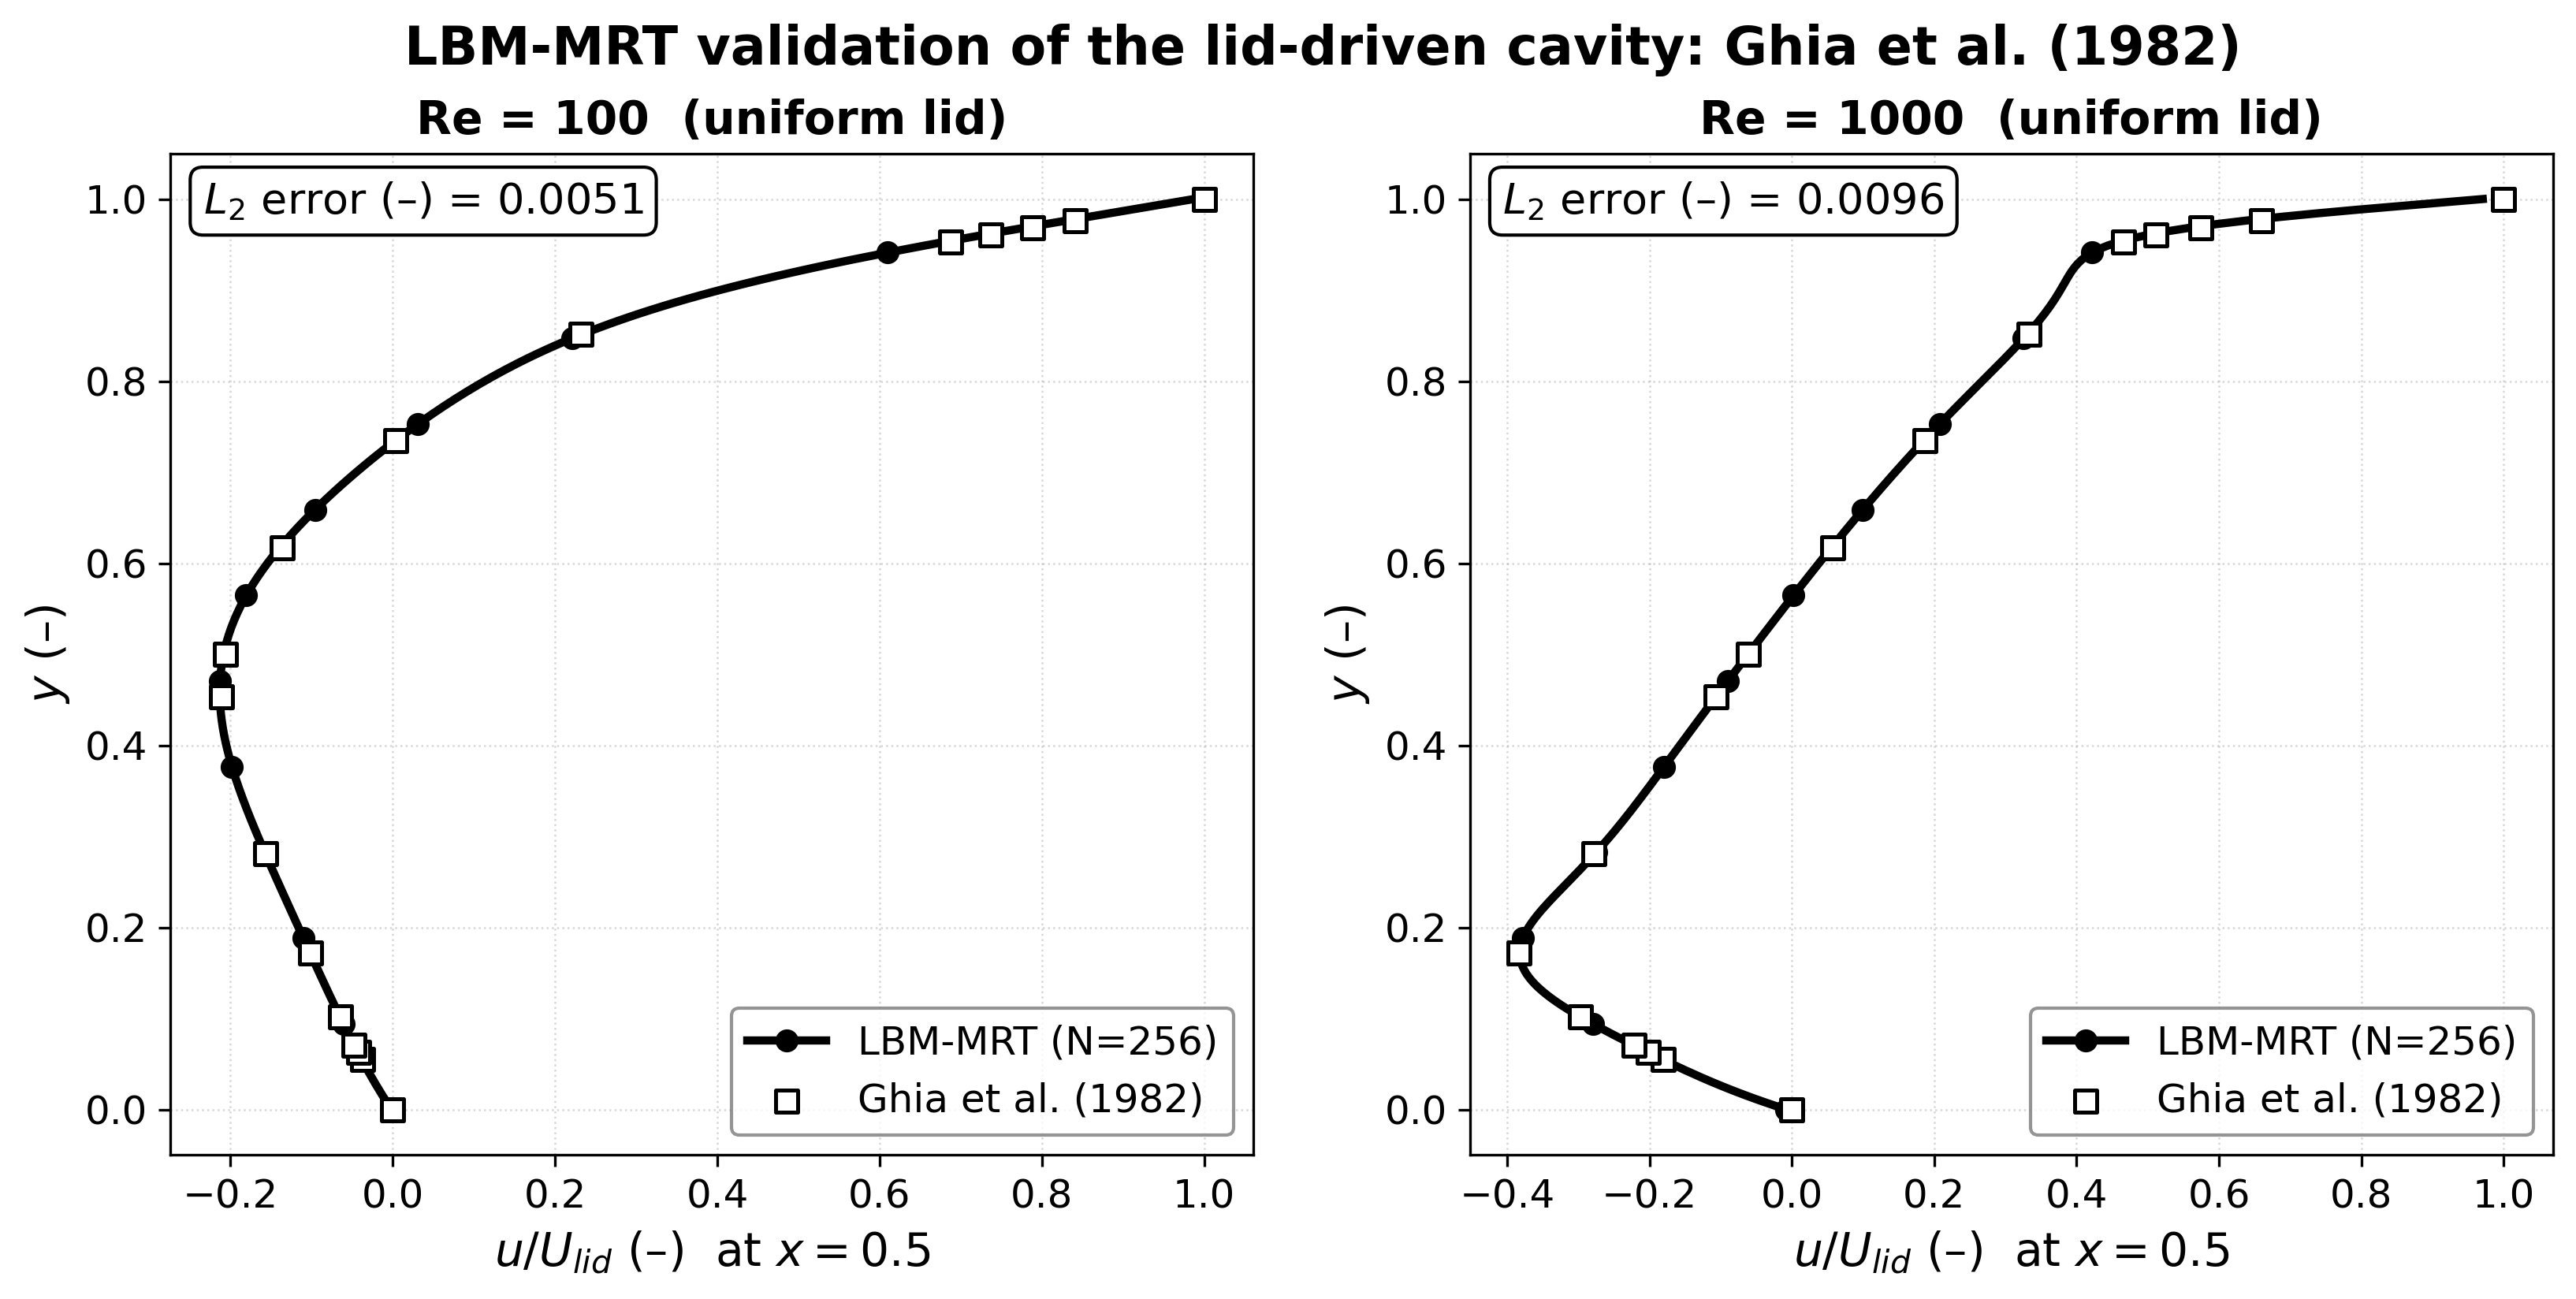
\includegraphics[width=\textwidth]{figS9_ghia_validation.png}
\caption{Square-cavity LBM center-line velocity profiles versus Ghia et al.\
(1982), $Re=100$ (left) and $Re=1000$ (right), uniform lid, $N=256$.
The in-panel $L_2$ values correspond to the center-line errors reported in
Table~\ref{tab:ghia}.}




\label{fig:ghia}
\end{figure}



\subsection{Curved-boundary test (exact rigid rotation)}
The curved-boundary implementation is verified against the exact stationary
solution $u=(y,-x)$ of a fully rotating disk, which is independent of $Re$.
At fixed lid velocity the $L_2$ error of this test stagnates near $10^{-3}$ as
the grid is refined, because the residual error is set by the lattice Mach
number of the fixed $U_{\mathrm{lid}}$. Table~\ref{tab:rotation} reports the same
test in a diffusive scaling, $U_{\mathrm{lid}}(N)=0.05\times32/N$, which keeps
$Re=100$ and $\tau\simeq0.547$ fixed while the lattice Mach number decreases as
$1/N$. The error then decreases monotonically, with observed orders $1.88$,
$1.90$ and $1.93$ between successive grids. The companion
fixed-$U_{\mathrm{lid}}$ runs corroborate the lattice-Mach interpretation
through the wall-normal leakage $\max|u\cdot m|$, which decreases from
$4.41\times10^{-5}$ at $N=32$ to $2.06\times10^{-5}$ at $N=96$. The production
campaign holds $U_{\mathrm{lid}}=0.05$ at every resolution, so this test
supports caution about a lattice-Mach offset but does not determine its effect
on production gradients. A production-family diffusive-scaling check is
reported in Sec.~\ref{sec:diffusive}: it leaves the junction-excised values
essentially unchanged and does not support a Mach/acoustic explanation of the
remaining drift. Two reported ranges refer to different sampled sets and should
not be mixed: $18.1$--$25.4\,\%$ is an average over seven sampled Reynolds
numbers, whereas $19.5$--$25.6\,\%$ is a different set of
representative $N=128$/$256$ pairs. In the
fixed-cutoff comparison of Sec.~S8 the median $D_{256}/D_{128}-1$ decreases from
$21.37\%$ at $r_0=0$ to $8.77\%$ at $r_0=0.5$; none of these ranges is an error
relative to a converged continuum solution.
% ------------------------------------------------------------------
\begin{table}[H]
\centering
\caption{Curved-boundary verification on the exact rigid-rotation solution
$u=(y,-x)$ of a rotating disk at $Re=100$, in diffusive scaling
$U_{\mathrm{lid}}(N)=0.05\times32/N$: $L_2$/$L_\infty$ errors, lid velocity,
iterations and final residual.}




\label{tab:rotation}
\begin{tabular}{@{}lccccc@{}}
\toprule
$N$ & $U_{\mathrm{lid}}$ & $L_2$ & $L_\infty$ & Iterations & Residual \\
\midrule
32 & 0.0500 & $9.35\times10^{-4}$ & $1.29\times10^{-3}$ & 18\,500 & $9.57\times10^{-11}$ \\
48 & 0.0333 & $4.36\times10^{-4}$ & $5.95\times10^{-4}$ & 38\,900 & $9.96\times10^{-11}$ \\
64 & 0.0250 & $2.52\times10^{-4}$ & $3.42\times10^{-4}$ & 65\,800 & $9.78\times10^{-11}$ \\
96 & 0.0167 & $1.15\times10^{-4}$ & $1.55\times10^{-4}$ & 136\,700 & $9.97\times10^{-11}$ \\
\bottomrule
\end{tabular}
\end{table}


\subsection{LBM--FEM cross-validation over the superelliptic family}
\label{sec:solverc}

To validate the MRT-LBM solver across the geometric family, an independent cross-validation is performed against a Taylor--Hood quadratic-velocity/linear-pressure (P2/P1) finite-element solver. Table~\ref{tab:lbmfem} reports interior relative $L_2$ discrepancies at the available $(N,Re)$ comparison levels, including the reference resolution $N=128$ at $Re=400$ for the sharpest
member ($n=1.25$, discrepancy $1.39\%$) and the near-square member ($n=4$,
discrepancy $0.78\%$). At fixed finite-element mesh, halving the lattice spacing
reduces the $n=4$ discrepancy from $1.45\%$ to $0.78\%$, locating the dominant
remaining difference on the lattice side. The pointed tip remains the worst
case, consistent with the tighter radius of curvature resolved by the
interpolated bounce-back scheme. The additional $N=256$ comparison decreases the
discrepancy to $0.60\%$ and $0.25\%$, but refines both discretisations and
therefore does not attribute the residual to either side.

The resolution study in Fig.~\ref{fig:lbmfemconv} shows that the interior LBM--FEM discrepancy decreases from $1.48\times10^{-2}$ at $N=32$ to $2.20\times10^{-3}$ at $N=96$ on the circle at $Re=100$. This decrease is reported as a sensitivity check over the tested grids; it is not used to claim a converged asymptotic error or to transfer a formal convergence rate to the production cases.


% ------------------------------------------------------------------
\begin{table}[H]
\centering
\caption{Interior relative $L_2$ discrepancy (\%) between MRT-LBM and the
independent Taylor--Hood $\mathbb{P}_2/\mathbb{P}_1$ FEM solution, tabulated by
comparison level. The lattice resolution $N$ and the finite-element refinement
$n_{\mathrm{refs}}$ are independent discretisation levels and are not matched
to one another; each row therefore states the mesh it actually used, as
triangle and total-unknown counts ($2(V+E)+V$) measured on the assembled
mesh, so that the finite-element side of every comparison is fully specified.
$N=64$ at $Re=100$ and $N=96$ at $Re=400$ are the original cross-checks;
$N=128$ at $Re=400$ brings the comparison to the reference resolution of the
database and $n=1.25$ to the family, and it is made against the same
$74\,371$-unknown mesh as the $N=96$ row; $N=256$ at $Re=400$ is an additional
refined comparison, and because it refines the lattice and the finite-element
mesh together ($65\,536$ triangles, $296\,195$ unknowns) it cannot attribute the
residual to either side --- it only checks that the discrepancy decreases and
that the pointed tip stays the worst of the family. At that level the
discrepancy is evaluated on the intersection of the two discretisations: $24$
of the $60\,132$ LBM fluid nodes of the $n=4$ case fall outside the assembled
triangulation and are excluded from both metrics, against $0$ for $n=1.25$.
All LBM residuals are below $10^{-8}$; every FEM solve converged, in $22$ Picard
iterations at $n_{\mathrm{refs}}=6$ and in $18$ and $22$ at
$n_{\mathrm{refs}}=7$.}




\label{tab:lbmfem}
\tabbox{%
\begin{tabular}{@{}lccccc@{}}
\toprule
comparison level & $n=1.25$ & $n=1.5$ & $n=2$ & $n=4$ & square \\
\midrule
$Re=100$, $N=64$, $n_{\mathrm{refs}}=5$, $4\,096$ triangles, $18\,755$ unknowns & -- & 1.06 & 0.93 & 0.96 & 0.87 \\
$Re=400$, $N=96$, $n_{\mathrm{refs}}=6$, $16\,384$ triangles, $74\,371$ unknowns & -- & 1.20 & 1.20 & 1.45 & 1.21 \\
$Re=400$, $N=128$, $n_{\mathrm{refs}}=6$, $16\,384$ triangles, $74\,371$ unknowns & 1.39 & -- & -- & 0.78 & -- \\
$Re=400$, $N=256$, $n_{\mathrm{refs}}=7$, $65\,536$ triangles, $296\,195$ unknowns & 0.60 & -- & -- & 0.25 & -- \\
\bottomrule
\end{tabular}%
}
\end{table}


\begin{figure}[H]
\centering
\begin{subfigure}[b]{0.48\textwidth}
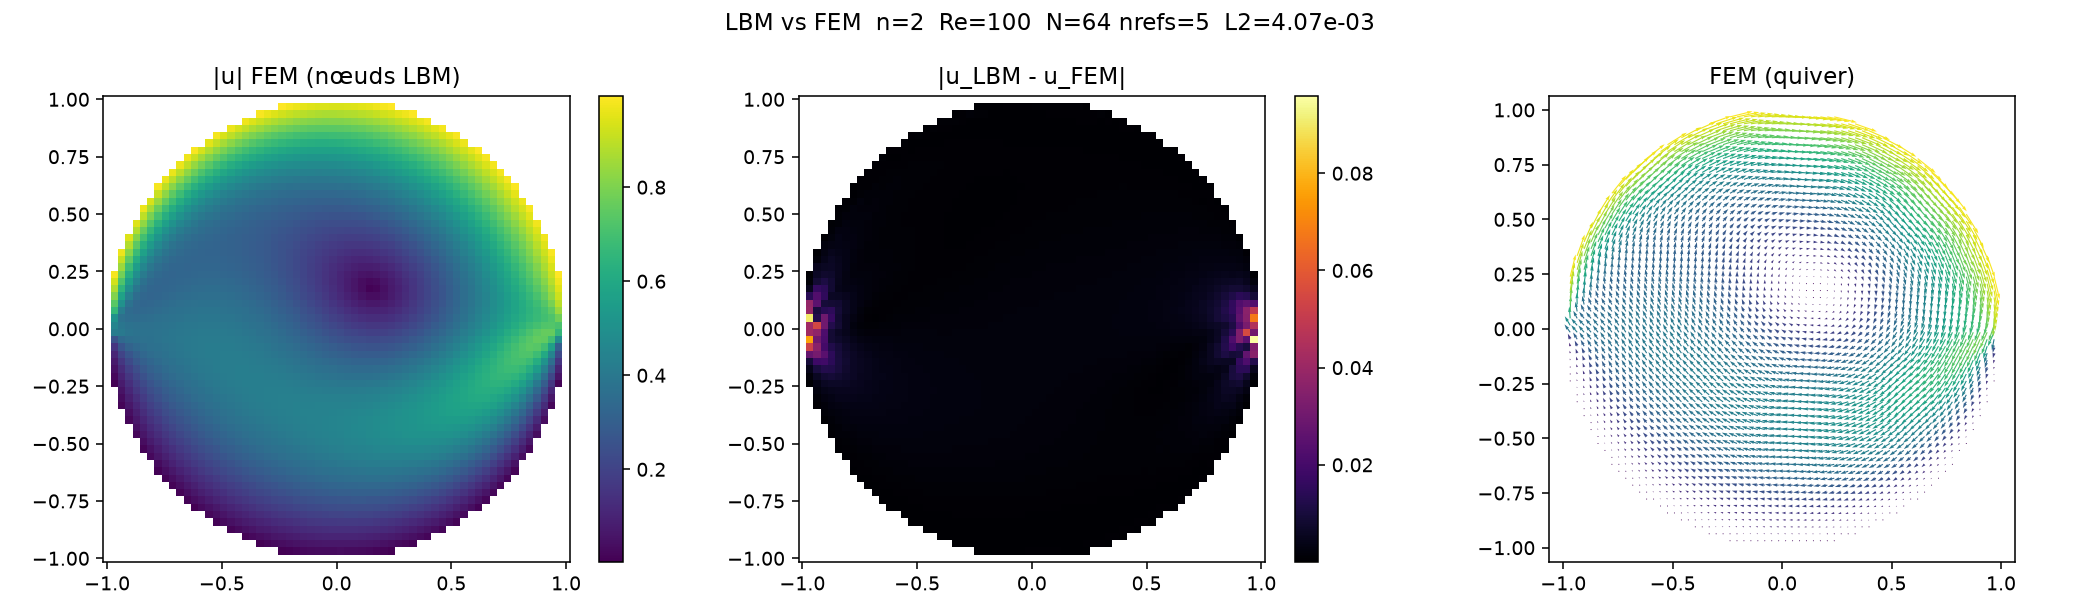
\includegraphics[width=\textwidth]{lbm_fem_circle_Re100_N64.png}
\caption{Circle ($n=2$), $Re=100$}
\end{subfigure}
\hfill
\begin{subfigure}[b]{0.48\textwidth}
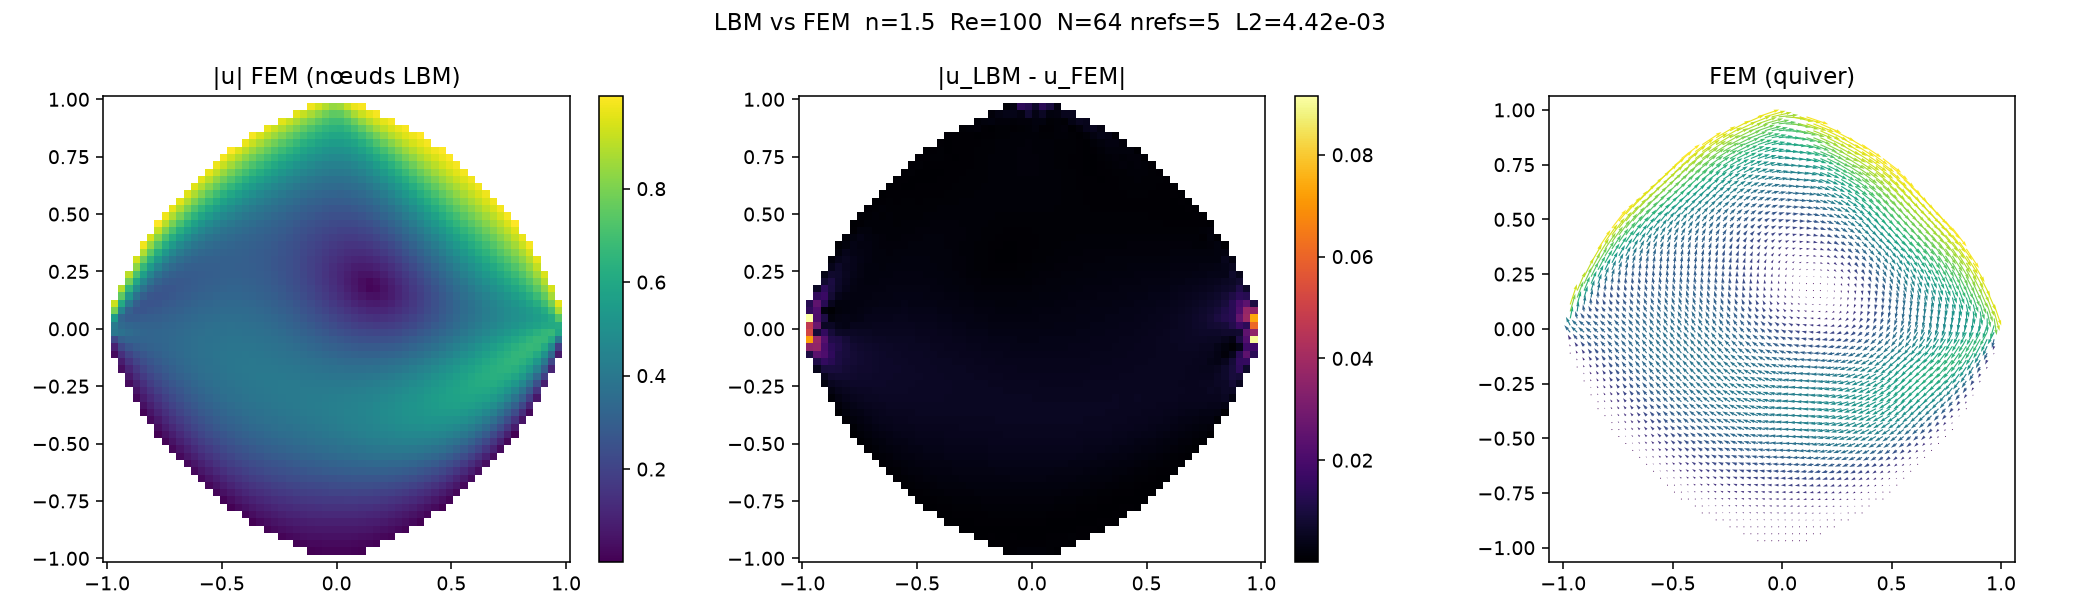
\includegraphics[width=\textwidth]{lbm_fem_ell1.5_Re100_N64.png}
\caption{Ellipse ($n=1.5$), $Re=100$}
\end{subfigure}
\vspace{0.3cm}
\begin{subfigure}[b]{0.48\textwidth}
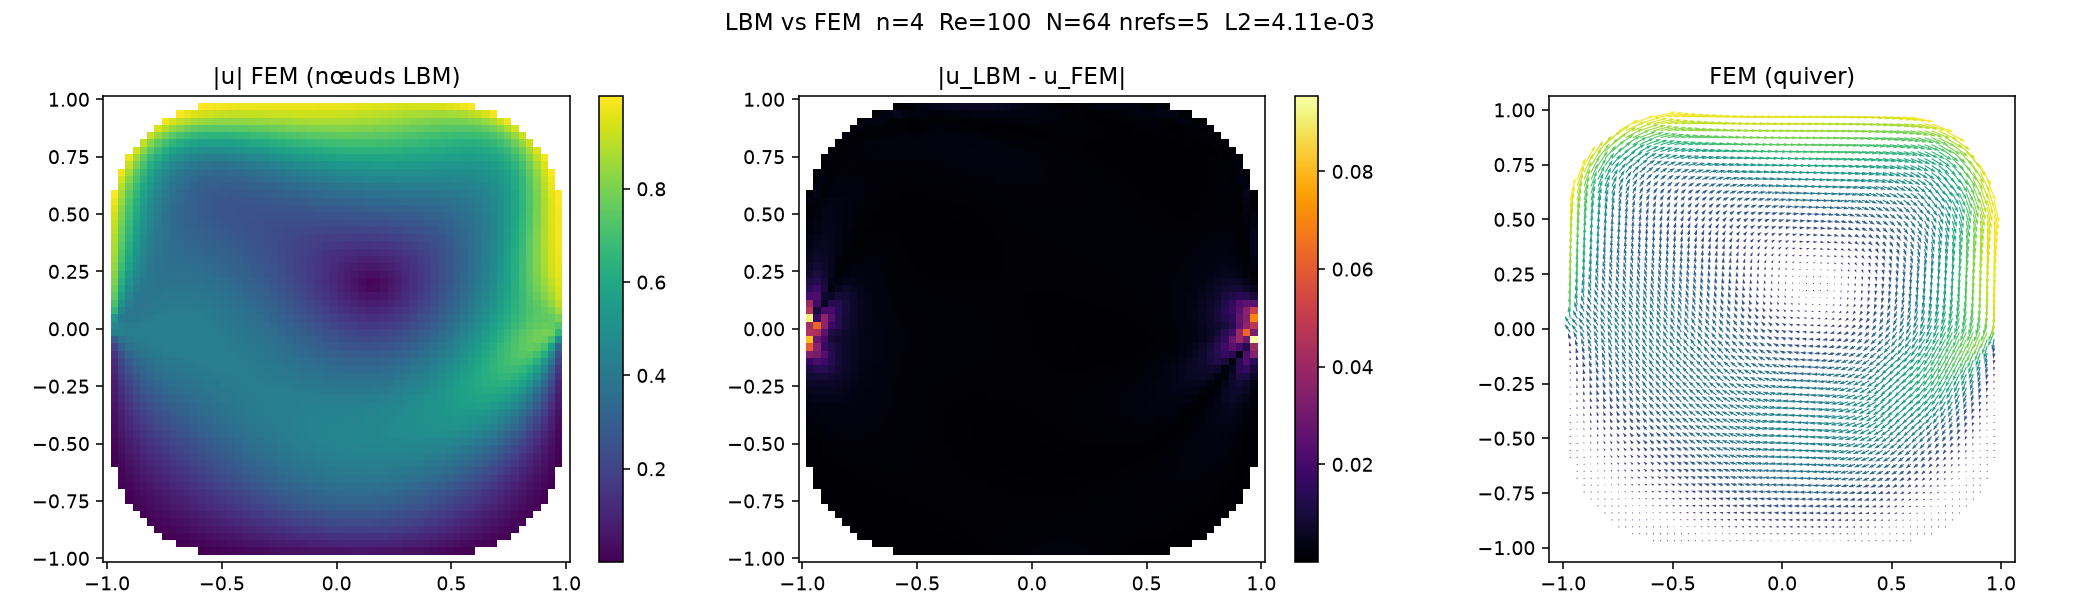
\includegraphics[width=\textwidth]{lbm_fem_ell4_Re100_N64.png}
\caption{Super-ellipse ($n=4$), $Re=100$}
\end{subfigure}
\hfill
\begin{subfigure}[b]{0.48\textwidth}
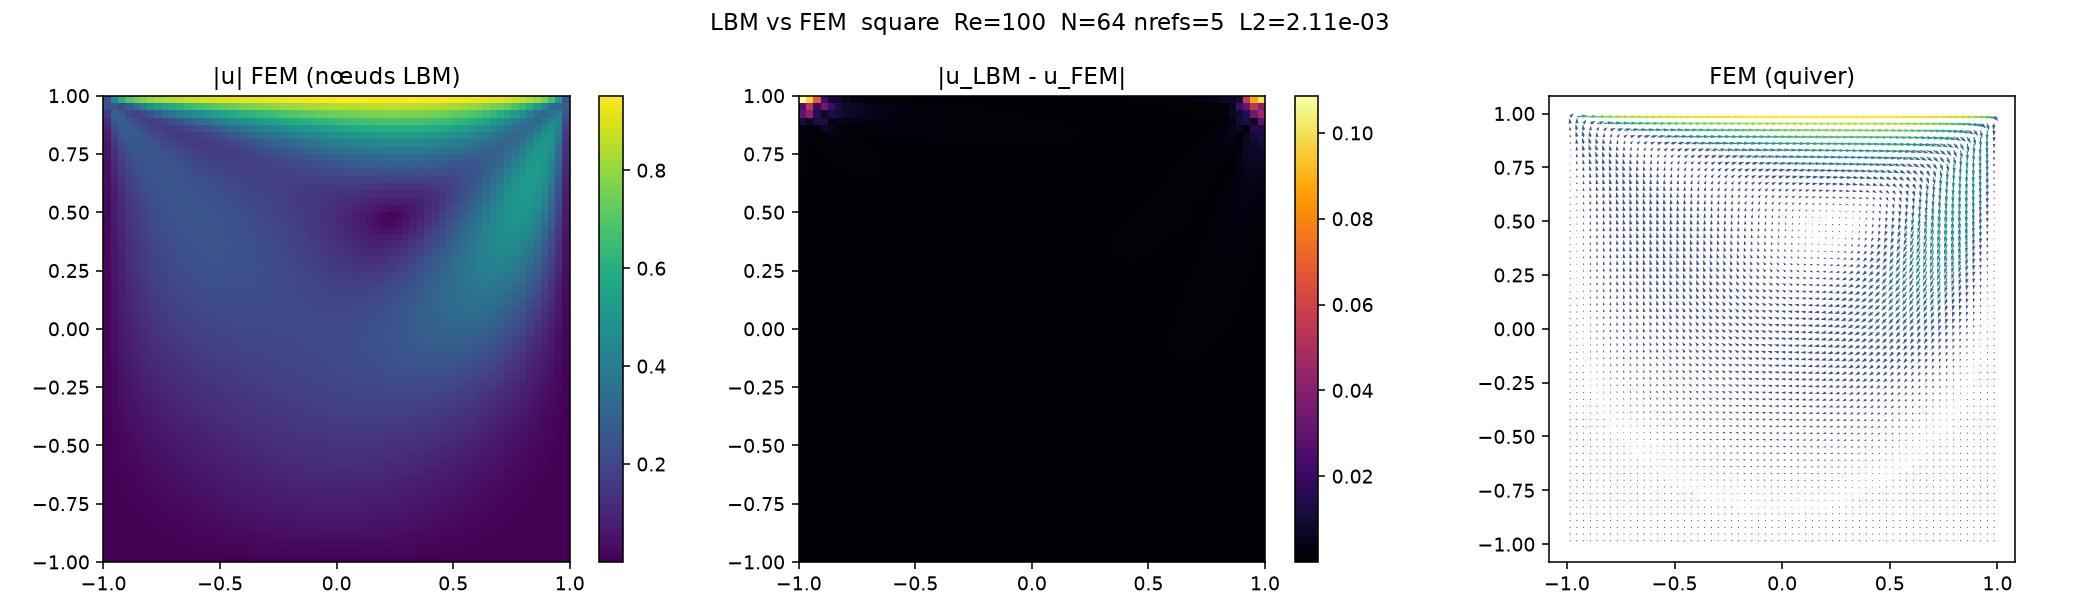
\includegraphics[width=\textwidth]{lbm_fem_square_Re100_N64.png}
\caption{Square, $Re=100$}
\end{subfigure}
\caption{LBM--FEM velocity-field comparison at $Re=100$ for four cavity geometries
(lattice $N=64$, finite-element mesh $n_{\mathrm{refs}}=5$, $4\,096$ triangles). Each panel overlays the LBM and FEM
streamlines on the LBM velocity magnitude. The corresponding interior relative
$L_2$ discrepancies are reported in Table~\ref{tab:lbmfem}.}




\label{fig:lbmfem100}
\end{figure}


\begin{figure}[H]
\centering
\begin{subfigure}[b]{0.48\textwidth}
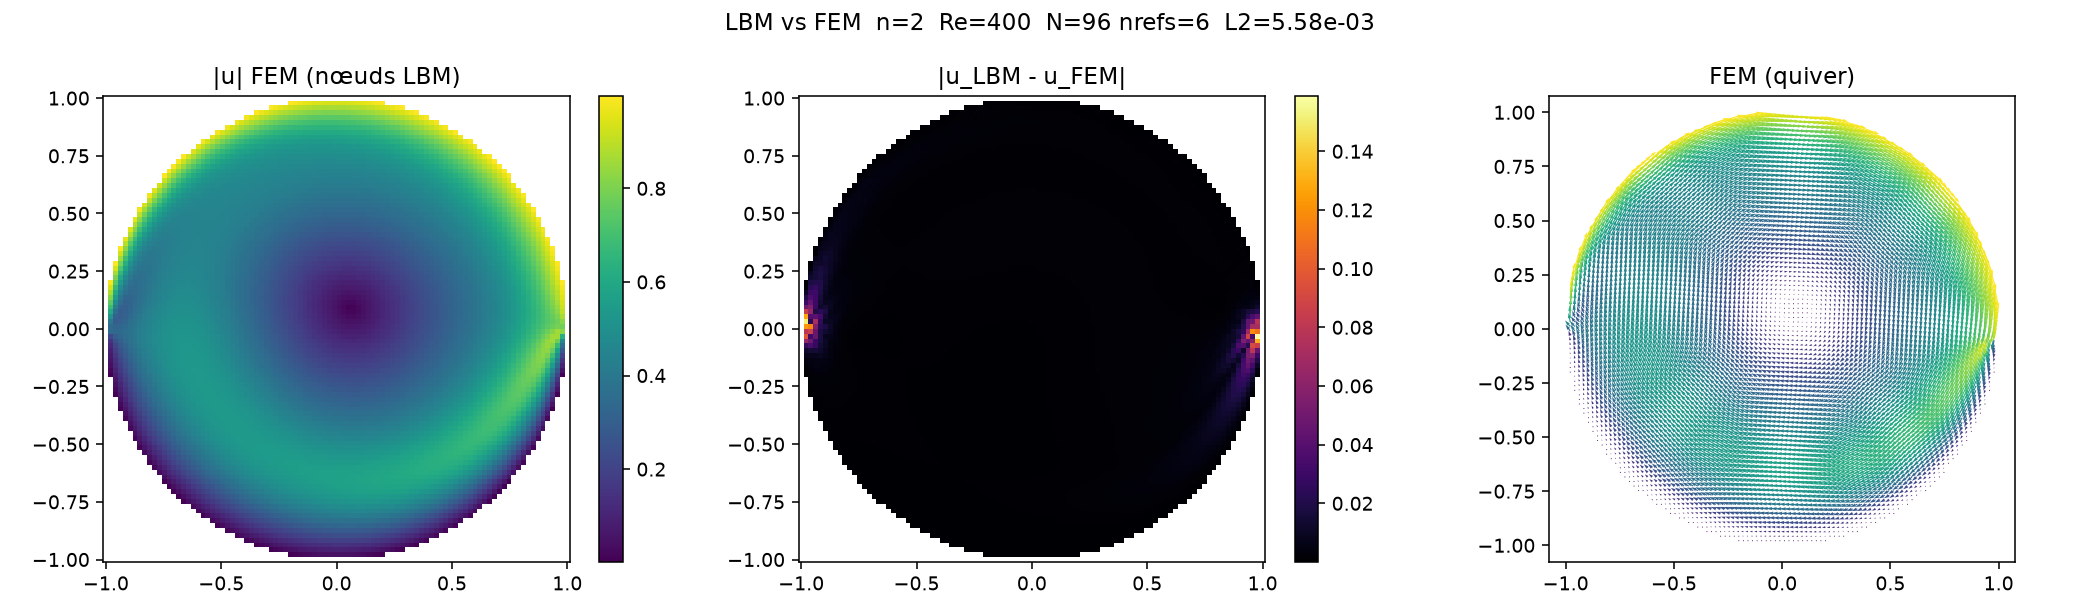
\includegraphics[width=\textwidth]{lbm_fem_circle_Re400_N96.png}
\caption{Circle ($n=2$), $Re=400$}
\end{subfigure}
\hfill
\begin{subfigure}[b]{0.48\textwidth}
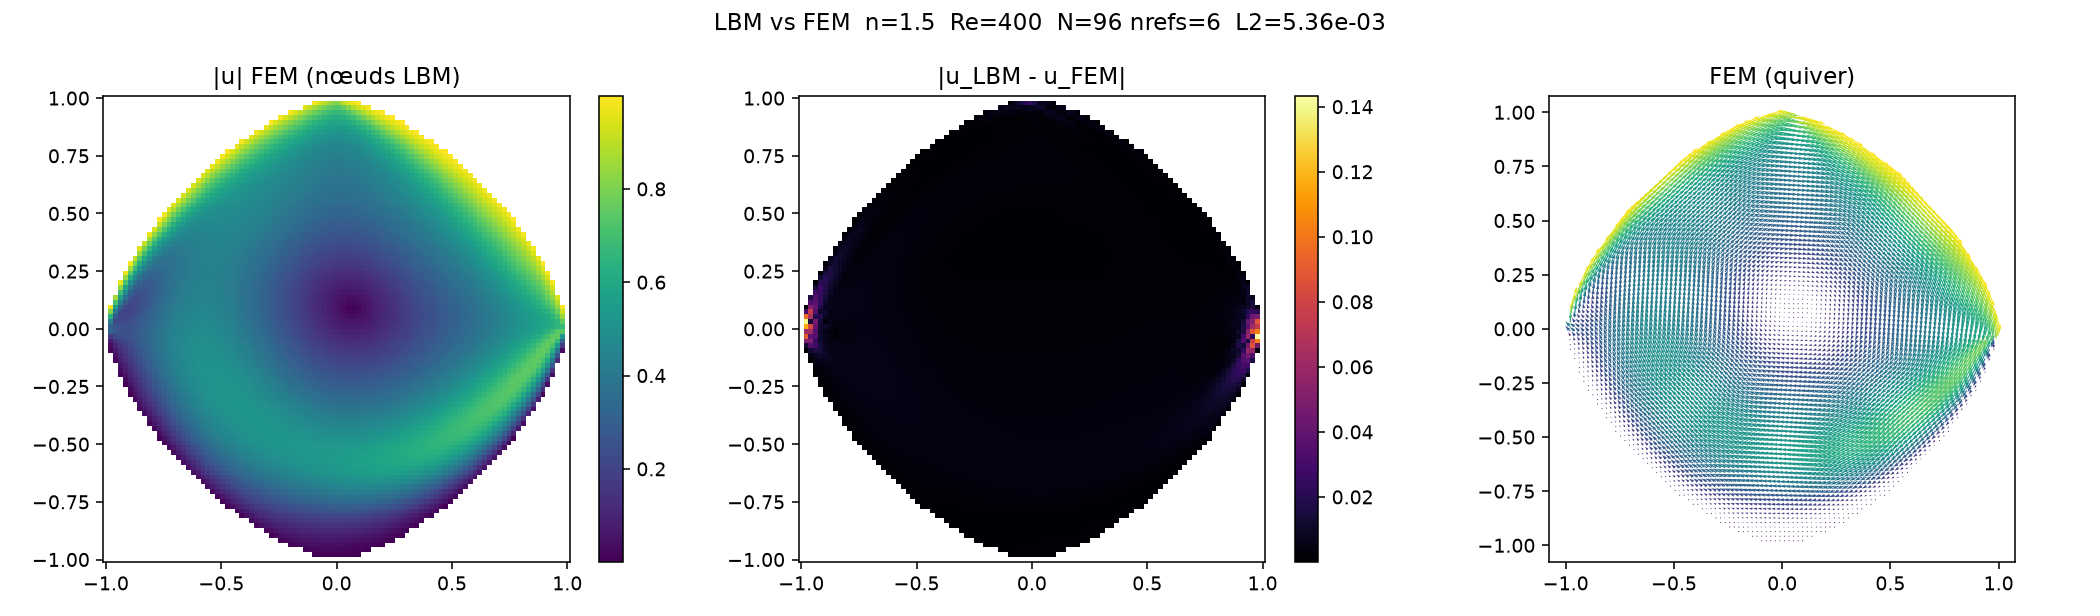
\includegraphics[width=\textwidth]{lbm_fem_ell1.5_Re400_N96.png}
\caption{Ellipse ($n=1.5$), $Re=400$}
\end{subfigure}
\vspace{0.3cm}
\begin{subfigure}[b]{0.48\textwidth}
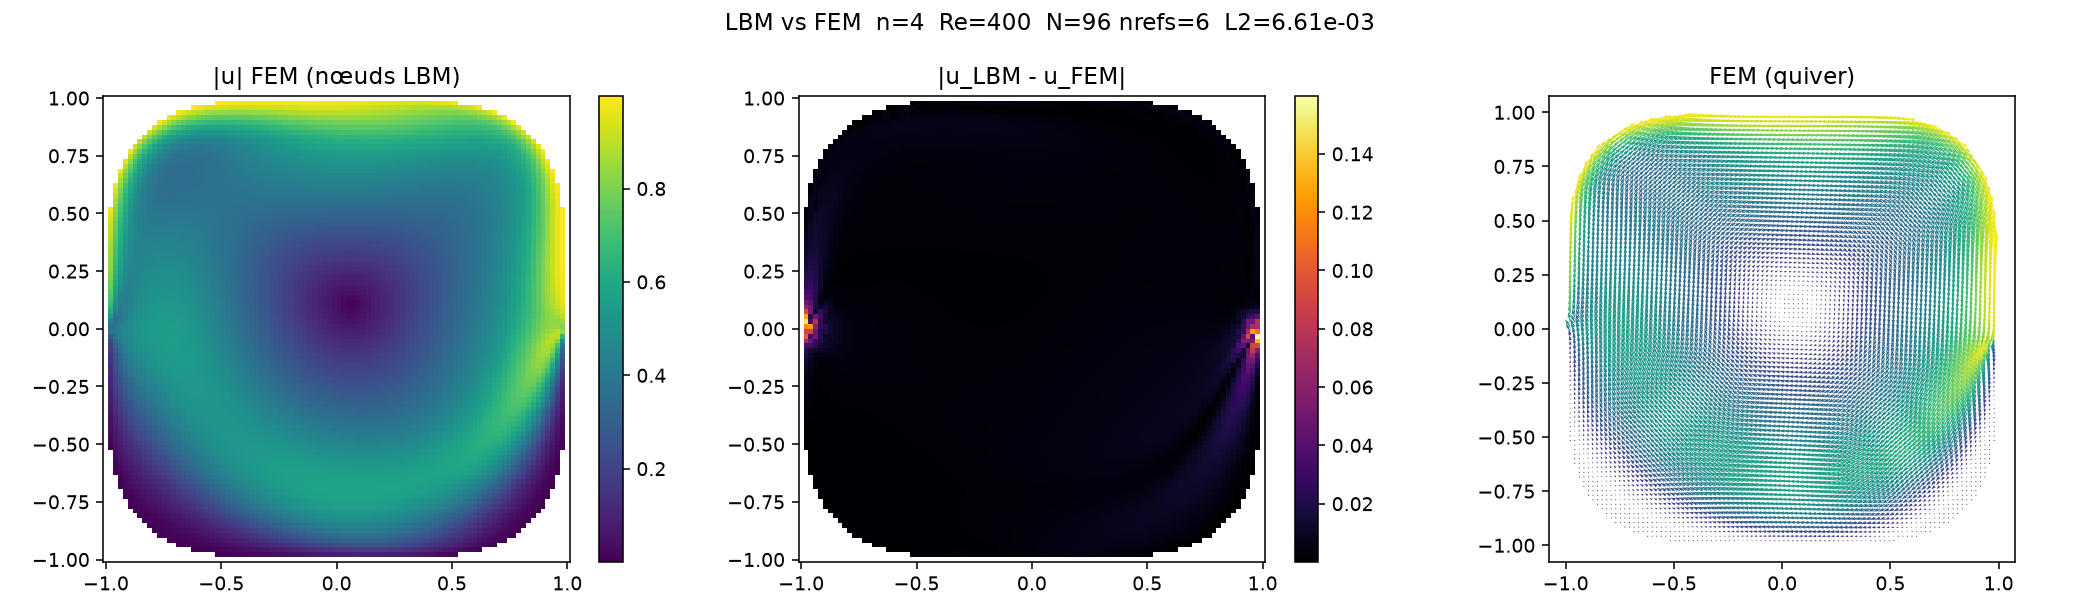
\includegraphics[width=\textwidth]{lbm_fem_ell4_Re400_N96.png}
\caption{Super-ellipse ($n=4$), $Re=400$}
\end{subfigure}
\hfill
\begin{subfigure}[b]{0.48\textwidth}
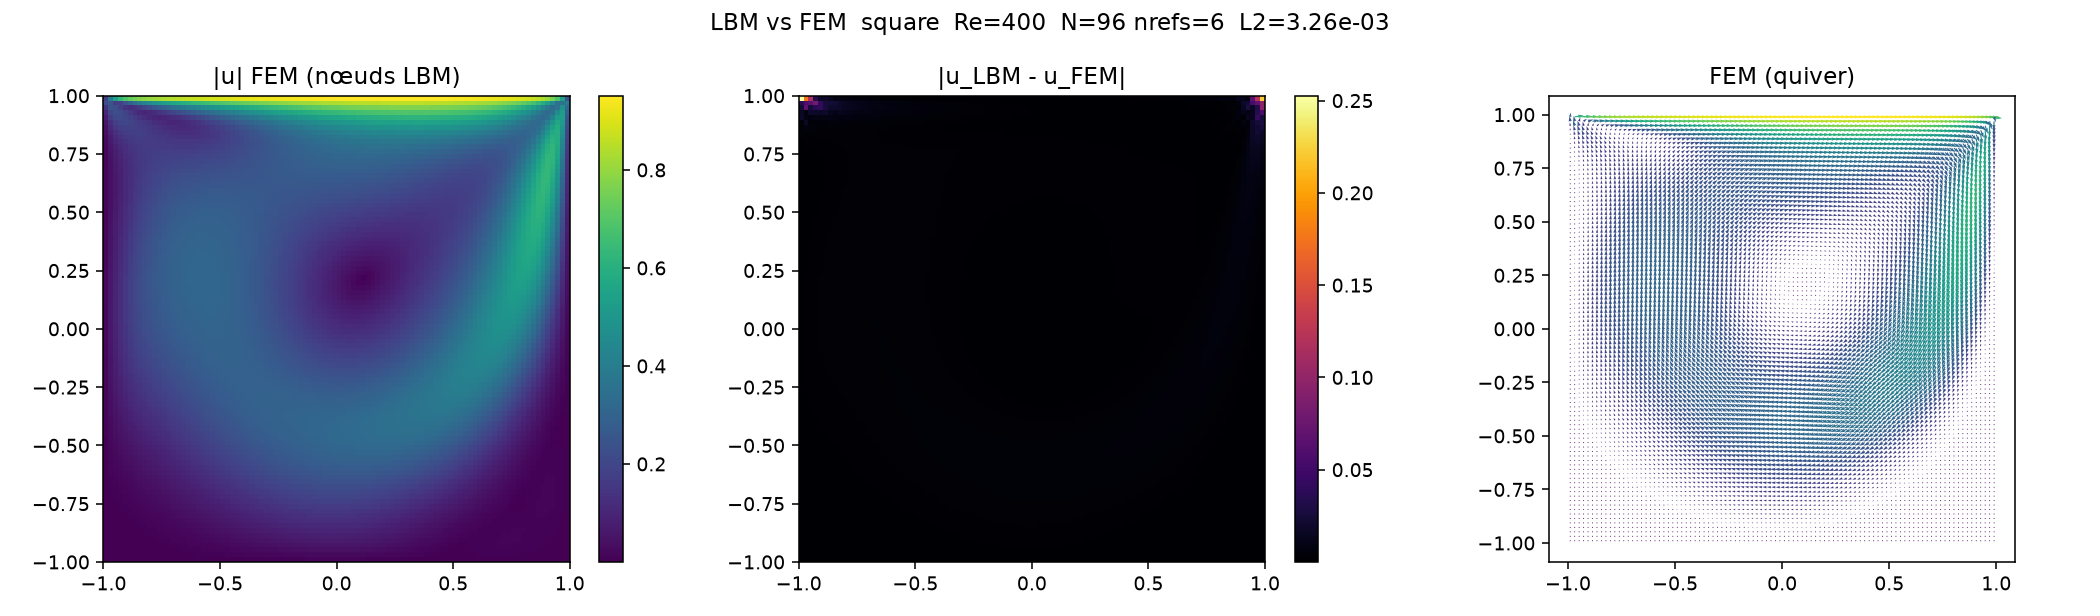
\includegraphics[width=\textwidth]{lbm_fem_square_Re400_N96.png}
\caption{Square, $Re=400$}
\end{subfigure}
\caption{LBM--FEM velocity-field comparison at $Re=400$ for four cavity geometries
(lattice $N=96$, finite-element mesh $n_{\mathrm{refs}}=6$, $16\,384$ triangles). The comparison remains within the reported
discretization-error range, with all interior relative $L_2$ discrepancies
below $1.5\,\%$ (Table~\ref{tab:lbmfem}).}




\label{fig:lbmfem400}
\end{figure}


\begin{figure}[H]
\centering
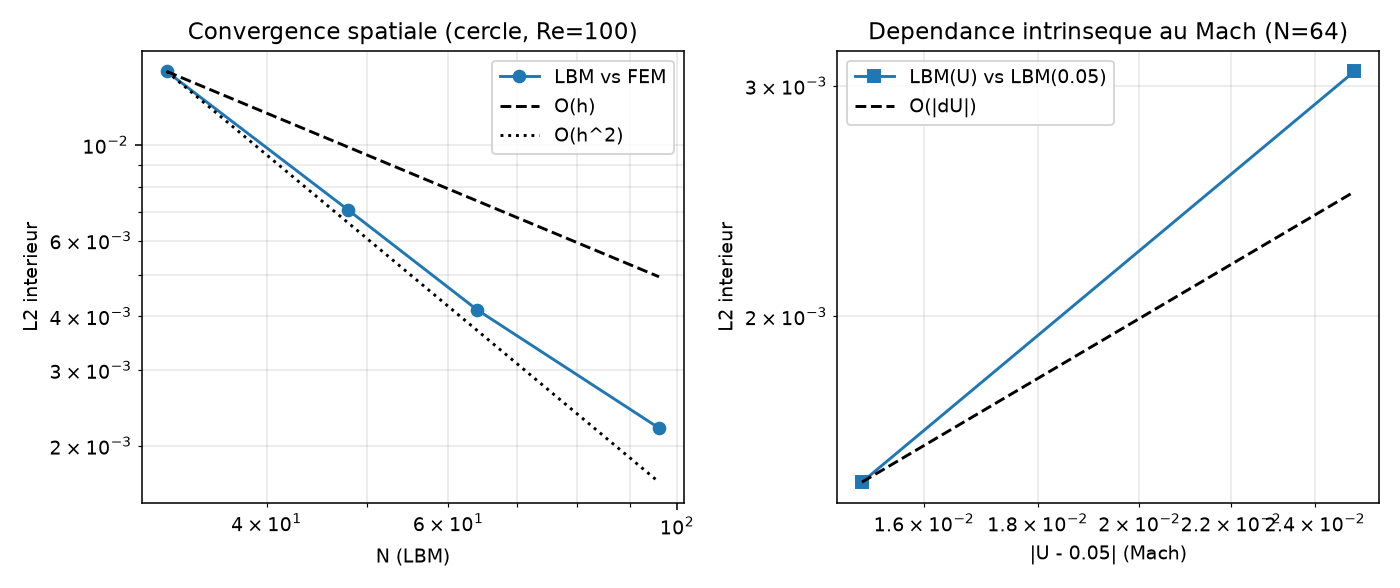
\includegraphics[width=0.70\textwidth]{figS11b_lbm_fem_convergence_N.png}
\caption{Grid dependence of the LBM--FEM interior relative $L_2$ discrepancy
for the circular cavity at $Re=100$ as the LBM resolution is refined from
$N=32$ to $N=96$. The observed decrease is consistent with a reduction of
discretization error over the tested resolutions.}




\label{fig:lbmfemconv}
\end{figure}


% ======================================================================

\section{Dataset consistency checks}\label{sec:database}
Every retained configuration in the $190$-case physics-analysis subset
passed the fixed consistency protocol before being included in the analysis;
this section details the results for
the $190$-case physics-analysis subset (all $10$ exponents $n$ at the $19$
Reynolds numbers of the complete grid, $N=128$). Table~\ref{tab:qc} condenses the
checks: $190$ cases found
and analysed, zero failures, maximum relative area error of the discretized
domain $0.948\,\%$ (below the $1\,\%$ acceptance threshold), maximum LBM residual
$9.9999\times10^{-9}$ (below $1\times10^{-8}$), and positive minimum density.
Because the tangential moving-lid boundary condition
$u_w=U_{\mathrm{lid}}(m_y,-m_x)$ is not invariant under reflection
$x\mapsto-x$, mirror symmetry is not a valid consistency criterion for
this dataset and is therefore excluded from this check
(\emph{not applicable} status). Fig.~\ref{fig:areaerror} shows the spatial
distribution of the area error over the $n\times Re$ grid.

The database maximum of the finite-difference divergence, $|\nabla\cdot u|=1.67$
(Table~\ref{tab:qc}), is attained at a single isolated interior cell of the most
pointed configuration ($n=1.25$, $Re=1000$), at $x\approx-0.953$,
$y\approx0.024$, i.e.\ about three cell widths from the wall in the sharp
curved-tip region; its four-point stencil is entirely fluid, so the value is
not a boundary-stencil artifact, but it is consistent with the strong local
curvature-approximation error of the curved moving boundary at the sharp
vertex. It is reported as a local, geometry-specific finite-resolution
excursion rather than a systematic feature of the database.

Recomputing the same diagnostic on the $50$-case $N=256$ campaign confirms
this reading. The per-case maximum scales with the stencil length, as expected
for a finite-difference derivative of a discrete field: its median over the
database rises from $1.31$ at $N=128$ ($190$ cases) to $2.43$ at $N=256$
($50$ cases). The individual outlier grows on that same trend, from $1.67$ to
$2.72$ --- a factor $1.63$, against $1.85$ for the median --- which is what a
tip-localised structure whose discrete gradient steepens with $h$ does, and not
what a spurious error does: refining resolves it further instead of removing
it. The case $(n,Re)=(1.25,1000)$ still carries the largest value,
$\max|\nabla\cdot u|=2.72$, but now by only $12\,\%$ above the $N=256$ median
(against $27\,\%$ at $N=128$), and the maximum migrates to the opposite tip
($x\approx0.977$, $y\approx0.012$) with the left--right asymmetry of the
tangential drive. The excursion is therefore a resolution-scaling
finite-difference signature of the sharp tip, not a physical divergence of
the field. Its weight in the reported observables is negligible: removing the
single worst cell changes $D/A$ by $-0.06\,\%$ at $N=128$ and $-0.07\,\%$ at
$N=256$, and removing the $20$ worst cells by $-4.2\,\%$ and $-2.6\,\%$
respectively.
% ------------------------------------------------------------------
\begin{table}[H]
\centering
\caption{Dataset consistency-check summary ($190$ cases analysed, $N=128$).}




\label{tab:qc}
\begin{tabular}{@{}lll@{}}
\toprule
Metric & Value & Status \\
\midrule
Cases found / analysed & 190 / 190 & --- \\
Failed cases & 0 & --- \\
Max.\ relative area error & $9.479\times10^{-3}$ & pass ($<10^{-2}$) \\
Max.\ LBM residual & $9.9999\times10^{-9}$ & pass ($<10^{-8}$) \\
Min.\ density $\rho_{\min}$ & $0.9954$ & pass ($>0$) \\
Max.\ $|\nabla\cdot u|$ & $1.67$ & reported \\
Mirror symmetry & not applicable & excluded (tangent-lid boundary condition) \\
\bottomrule
\end{tabular}
\end{table}


\begin{figure}[H]
\centering
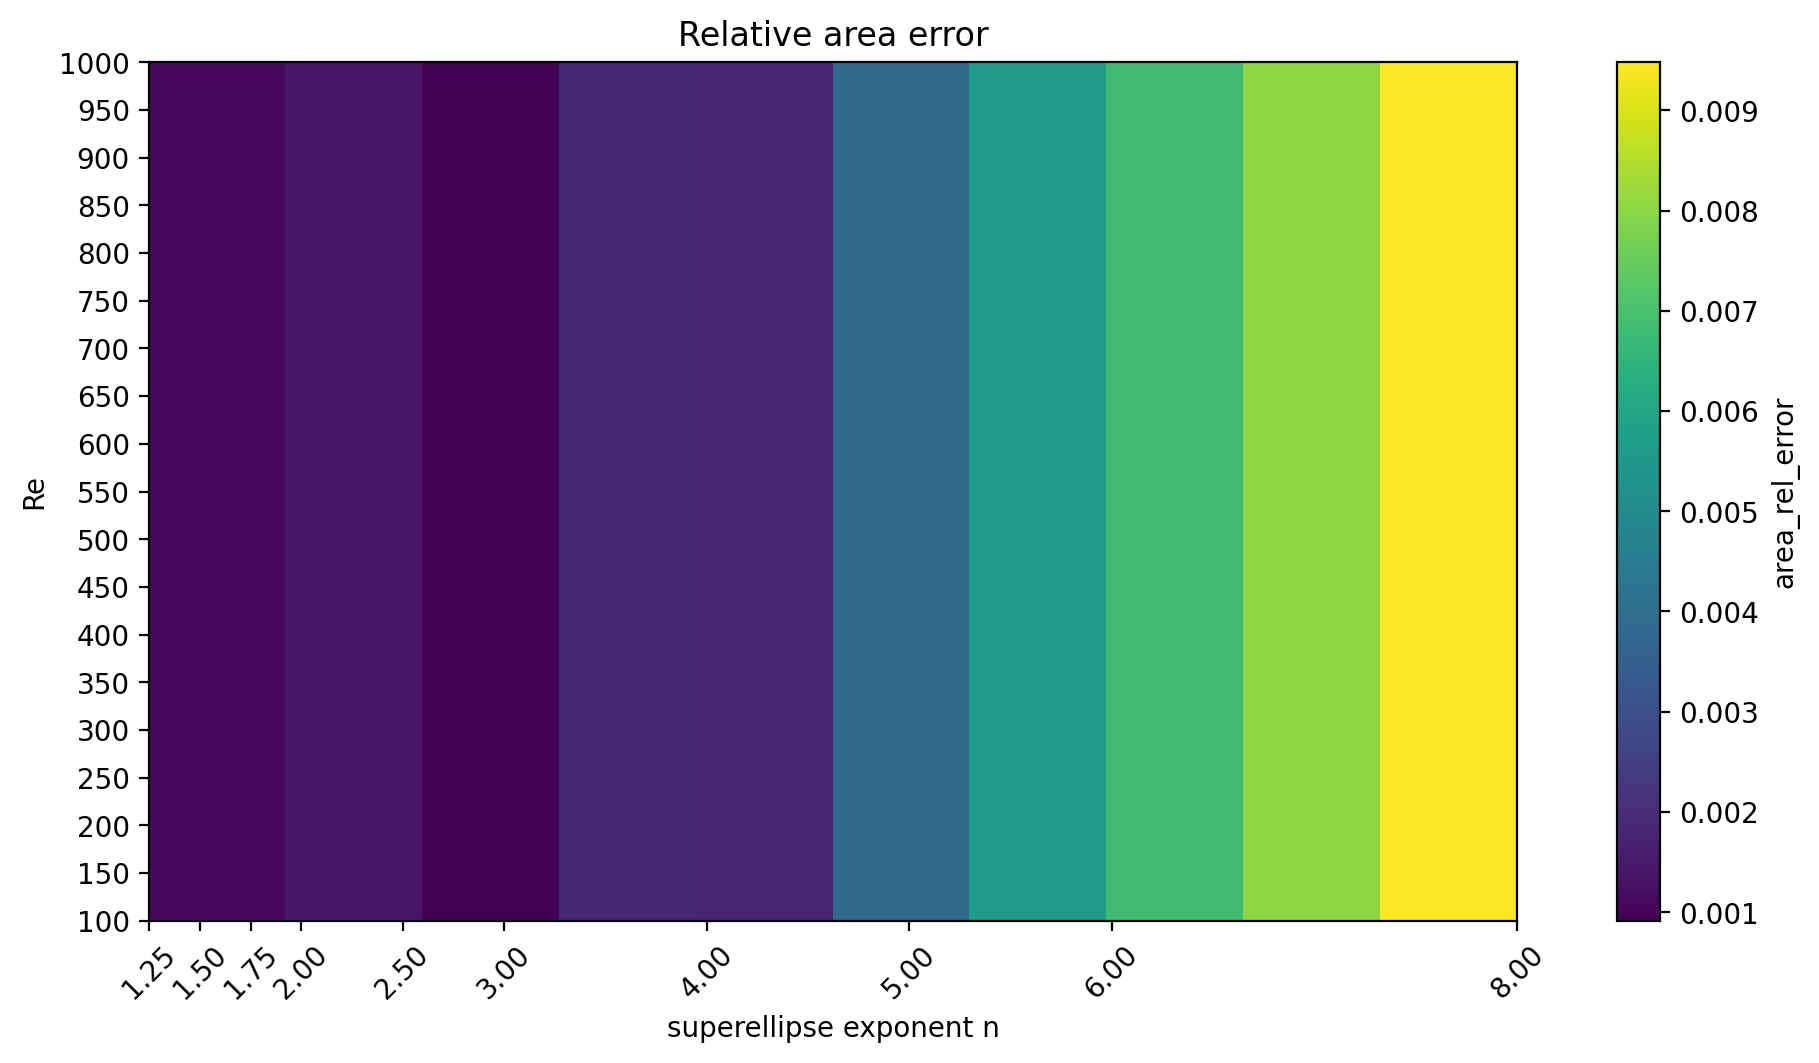
\includegraphics[width=\textwidth]{map_area_error.png}
\caption{Relative area error of the discretized domain over the
$n\times Re$ grid of the analysed subset. All
values are below the $1\,\%$ threshold.}




\label{fig:areaerror}
\end{figure}



\section{Physical observables of the comparison configurations}\label{sec:observables}
All physical observables reported in this section are computed from the
$N=128$ LBM reference fields.
The velocity derivatives are evaluated by second-order central differences on
the interior nodes whose four-point stencil is entirely fluid; the vorticity
is $\omega=\partial v/\partial x-\partial u/\partial y$; the streamfunction is
a diagnostic reconstruction obtained from the Poisson problem
$\nabla^2\psi=-\omega$ with $\psi=0$ on the discrete fluid boundary
(convention $u=\psi_y$, $v=-\psi_x$); the kinetic energy is
$KE=\int_{\Omega}\tfrac{1}{2}|\mathbf{u}|^2\,dA$ over the fluid mask; the
viscous dissipation is the standard mechanical dissipation of the
incompressible Newtonian fluid, $D=2\nu\int_{\Omega}S:S\,dA$, which evaluates
with $\nu=2/Re$ as
$D=\tfrac{4}{Re}\int_{\Omega}\left[(\partial u/\partial x)^2
+(\partial v/\partial y)^2+\tfrac{1}{2}(\partial u/\partial y+\partial
v/\partial x)^2\right]dA$ over the valid-gradient mask; and the enstrophy is
$\mathcal{E}=\tfrac{1}{2}\int_{\Omega}\omega^2\,dA$. The maximum velocity is
$U_{\max}=\max_{\Omega}|\mathbf{u}|$. Vortex counts are obtained from the
connected extrema of $\psi$ on the fluid core (nodes at Euclidean distance
$\geq 2$ from the wall), with threshold
$\tau=\max\left(\tfrac{q}{100}\,|\psi_{\mathrm{primary}}|,\,10^{-14}\right)$
for $q\in\{1,3,5\}\,\%$. The area-normalized kinetic energy of Table~\ref{tab:energy30} is obtained by
dividing $KE$ by the exact cavity area $A(n)=4\,\Gamma(1+1/n)^2/\Gamma(1+2/n)$
for $a=b=1$ (the area formula in the main manuscript), whereas $D/A$ is
divided by the area $A_{\rm mask}(n)$ of the discrete integration mask that
carries the sum defining $D$, so that numerator and denominator share the same
support.

Table~\ref{tab:observables} provides numerical values of the physical observables
for four representative configurations spanning the geometry family. These
values facilitate quantitative inspection of the reference fields and summarize
the principal flow characteristics. The table includes maximum velocity,
maximum absolute vorticity, primary streamfunction, vortex counts at the
$1\,\%$ and $5\,\%$ thresholds, dissipation, kinetic energy, enstrophy and the
root-mean-square divergence of the reference fields. The physical trends over
the complete $n$--$Re$ parameter space are discussed in the physical-analysis
sections of the main manuscript.
% ------------------------------------------------------------------
\begin{table}[H]
\centering
\caption{Physical observables of the four comparison configurations
($N=128$): maximum speed, maximum
absolute vorticity, primary streamfunction, vortex count at the $1\,\%$ /
$5\,\%$ thresholds, dissipation, kinetic energy, enstrophy and
root-mean-square (RMS) divergence.}




\label{tab:observables}
\tabbox{%
\begin{tabular}{@{}lcccccccc@{}}
\toprule
Case & $U_{\max}$ & $|\omega|_{\max}$ & $\psi_{\mathrm{prim}}$ &
$n_{\mathrm{vort}}^{1\%}/n_{\mathrm{vort}}^{5\%}$ & Dissipation & KE &
Enstrophy & RMS$\;|\nabla\cdot u|$ \\
\midrule
$n=2,Re=400$           & 0.998 & 21.4  & $-0.337$ & 1 / 1 & 0.0467 & 0.357 & 7.69 & 0.0334 \\
$n=3,Re=1000$          & 1.039 & 24.6  & $-0.360$ & 1 / 1 & 0.0248 & 0.409 & 9.02 & 0.0408 \\
$n=5,Re=1000$          & 1.035 & 24.6  & $-0.363$ & 1 / 1 & 0.0265 & 0.422 & 9.33 & 0.0395 \\
$n=8,Re=1000$          & 1.027 & 24.5  & $-0.361$ & 2 / 1 & 0.0284 & 0.421 & 9.67 & 0.0391 \\
\bottomrule
\end{tabular}%
}
\end{table}


\subsection{Area-normalized kinetic energy and dissipation}
Table~\ref{tab:grid190} gives the per-case energy and dissipation values for all $190$ cases,
and Table~\ref{tab:energy30} lists the subset at the three central Reynolds numbers. The interpretation of those columns --- the
non-monotonicity of $D/A$, the geometry of its sampled minimum, and the
distinction between minimizing $D$ and minimizing $D/A$ --- is given in
the physical-analysis sections of the main text and is not repeated here. The
corresponding curvature and wall/core analyses are given in
Secs.~\ref{sec:curvature} and~\ref{sec:corewall}.

For reference, the aggregate range over the 30-case grid, rather than within
a single Reynolds number, is $KE/A\in[0.0915,0.1182]$, which is wider
than the $Re=1000$ band quoted in the main-text energy analysis because the
three Reynolds numbers occupy slightly different levels. These values provide
the numerical basis for the main-text statements and do not constitute a second
presentation of them.
% ------------------------------------------------------------------
\begin{table}[H]
\centering
\caption{Integrated kinetic energy $KE$ and integrated dissipation
$D=2\nu\int_{\Omega}S:S\,dA$ with $\nu=2/Re$, together with their
area-normalized counterparts on the 30-case reference grid ($N=128$).
$KE/A$ uses the exact cavity area $A(n)$; $D/A$ uses the area $A_{\rm mask}(n)$
of the discrete integration mask, so that numerator and denominator share the
same support. Absolute dissipation levels are resolution-sensitive; the table
is used only for geometry ordering at fixed resolution and observable
definition.}




\label{tab:energy30}
\begin{tabular}{@{}rrrrrrrr@{}}
\toprule
$n$ & $Re$ & $A(n)$ & $A_{\rm mask}(n)$ & $KE$ & $KE/A$ & $D$ & $D/A$ \\
\midrule
 1.25 &  100 &  2.4271 &  2.3530 &  0.2221 &  0.0915 &  0.1873 &  0.07959 \\
  1.5 &  100 &  2.7379 &  2.6546 &  0.2722 &  0.0994 &  0.1423 &  0.05360 \\
 1.75 &  100 &  2.9678 &  2.8808 &  0.3083 &  0.1039 &  0.1245 &  0.04320 \\
    2 &  100 &  3.1416 &  3.0474 &  0.3313 &  0.1055 &  0.1162 &  0.03814 \\
  2.5 &  100 &  3.3809 &  3.2796 &  0.3572 &  0.1057 &  0.1122 &  0.03421 \\
    3 &  100 &  3.5333 &  3.4204 &  0.3669 &  0.1038 &  0.1141 &  0.03335 \\
    4 &  100 &  3.7081 &  3.5821 &  0.3729 &  0.1006 &  0.1222 &  0.03412 \\
    5 &  100 &  3.8006 &  3.6654 &  0.3729 &  0.0981 &  0.1309 &  0.03571 \\
    6 &  100 &  3.8552 &  3.7121 &  0.3709 &  0.0962 &  0.1388 &  0.03739 \\
    8 &  100 &  3.9138 &  3.7617 &  0.3671 &  0.0938 &  0.1522 &  0.04047 \\
 1.25 &  400 &  2.4271 &  2.3530 &  0.2388 &  0.0984 &  0.0643 &  0.02733 \\
  1.5 &  400 &  2.7379 &  2.6546 &  0.2933 &  0.1071 &  0.0536 &  0.02019 \\
 1.75 &  400 &  2.9678 &  2.8808 &  0.3320 &  0.1119 &  0.0491 &  0.01705 \\
    2 &  400 &  3.1416 &  3.0474 &  0.3567 &  0.1135 &  0.0467 &  0.01534 \\
  2.5 &  400 &  3.3809 &  3.2796 &  0.3838 &  0.1135 &  0.0455 &  0.01388 \\
    3 &  400 &  3.5333 &  3.4204 &  0.3941 &  0.1115 &  0.0458 &  0.01340 \\
    4 &  400 &  3.7081 &  3.5821 &  0.4019 &  0.1084 &  0.0479 &  0.01336 \\
    5 &  400 &  3.8006 &  3.6654 &  0.4037 &  0.1062 &  0.0501 &  0.01366 \\
    6 &  400 &  3.8552 &  3.7121 &  0.4032 &  0.1046 &  0.0520 &  0.01400 \\
    8 &  400 &  3.9138 &  3.7617 &  0.4018 &  0.1027 &  0.0551 &  0.01465 \\
 1.25 & 1000 &  2.4271 &  2.3530 &  0.2461 &  0.1014 &  0.0329 &  0.01400 \\
  1.5 & 1000 &  2.7379 &  2.6546 &  0.3041 &  0.1111 &  0.0285 &  0.01073 \\
 1.75 & 1000 &  2.9678 &  2.8808 &  0.3454 &  0.1164 &  0.0266 &  0.00924 \\
    2 & 1000 &  3.1416 &  3.0474 &  0.3713 &  0.1182 &  0.0255 &  0.00835 \\
  2.5 & 1000 &  3.3809 &  3.2796 &  0.3986 &  0.1179 &  0.0248 &  0.00757 \\
    3 & 1000 &  3.5333 &  3.4204 &  0.4090 &  0.1158 &  0.0248 &  0.00725 \\
    4 & 1000 &  3.7081 &  3.5821 &  0.4186 &  0.1129 &  0.0256 &  0.00714 \\
    5 & 1000 &  3.8006 &  3.6654 &  0.4216 &  0.1109 &  0.0265 &  0.00723 \\
    6 & 1000 &  3.8552 &  3.7121 &  0.4211 &  0.1092 &  0.0272 &  0.00733 \\
    8 & 1000 &  3.9138 &  3.7617 &  0.4208 &  0.1075 &  0.0284 &  0.00755 \\
\bottomrule
\end{tabular}
\end{table}


\section{Reference flow field atlas}\label{sec:atlas}
This section complements the main-text reference-flow atlas by providing the reference LBM flow fields at the lower Reynolds number $Re=100$. Figure~\ref{fig:atlas100} shows the velocity magnitude and streamfunction, illustrating the steady characteristics for representative geometries. The corresponding fields and vortex topologies at $Re=1000$ are discussed in the main text.

\begin{figure}[H]
\centering
\begin{subfigure}[b]{0.32\textwidth}
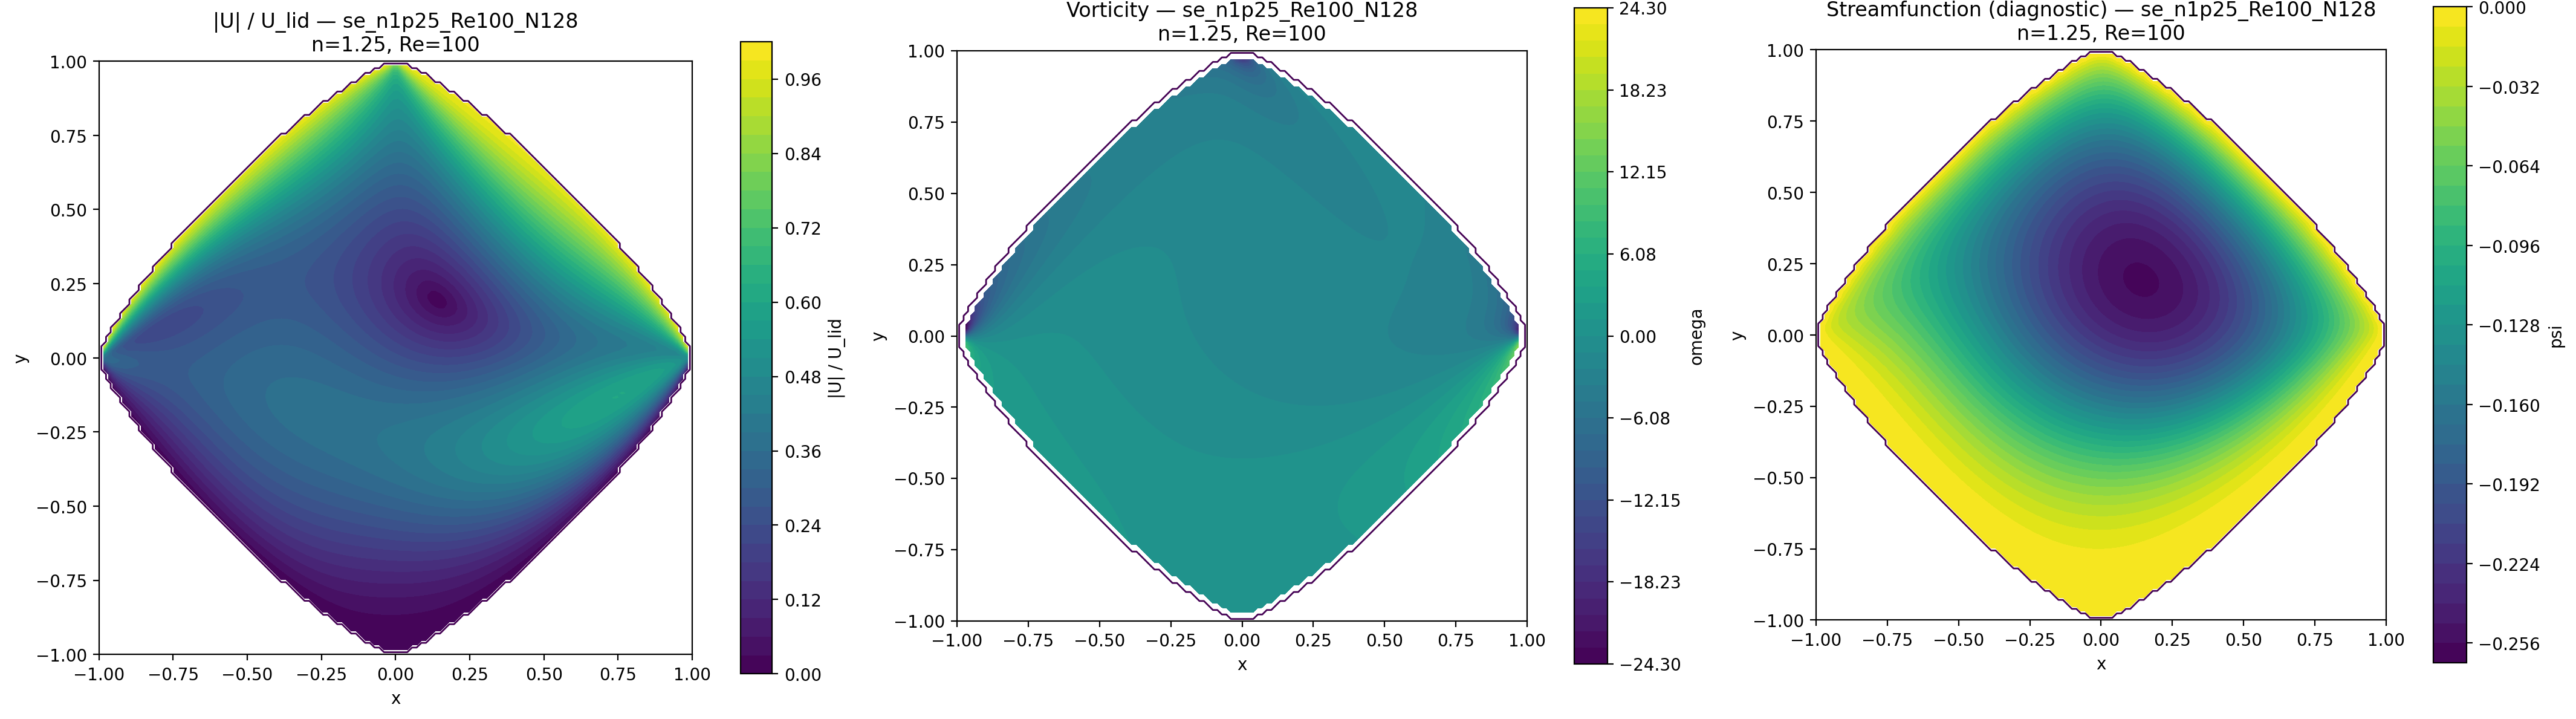
\includegraphics[width=\textwidth]{se_n1p25_Re100_N128_fields.png}
\caption{$n=1.25,\;Re=100$}
\end{subfigure}
\hfill
\begin{subfigure}[b]{0.32\textwidth}
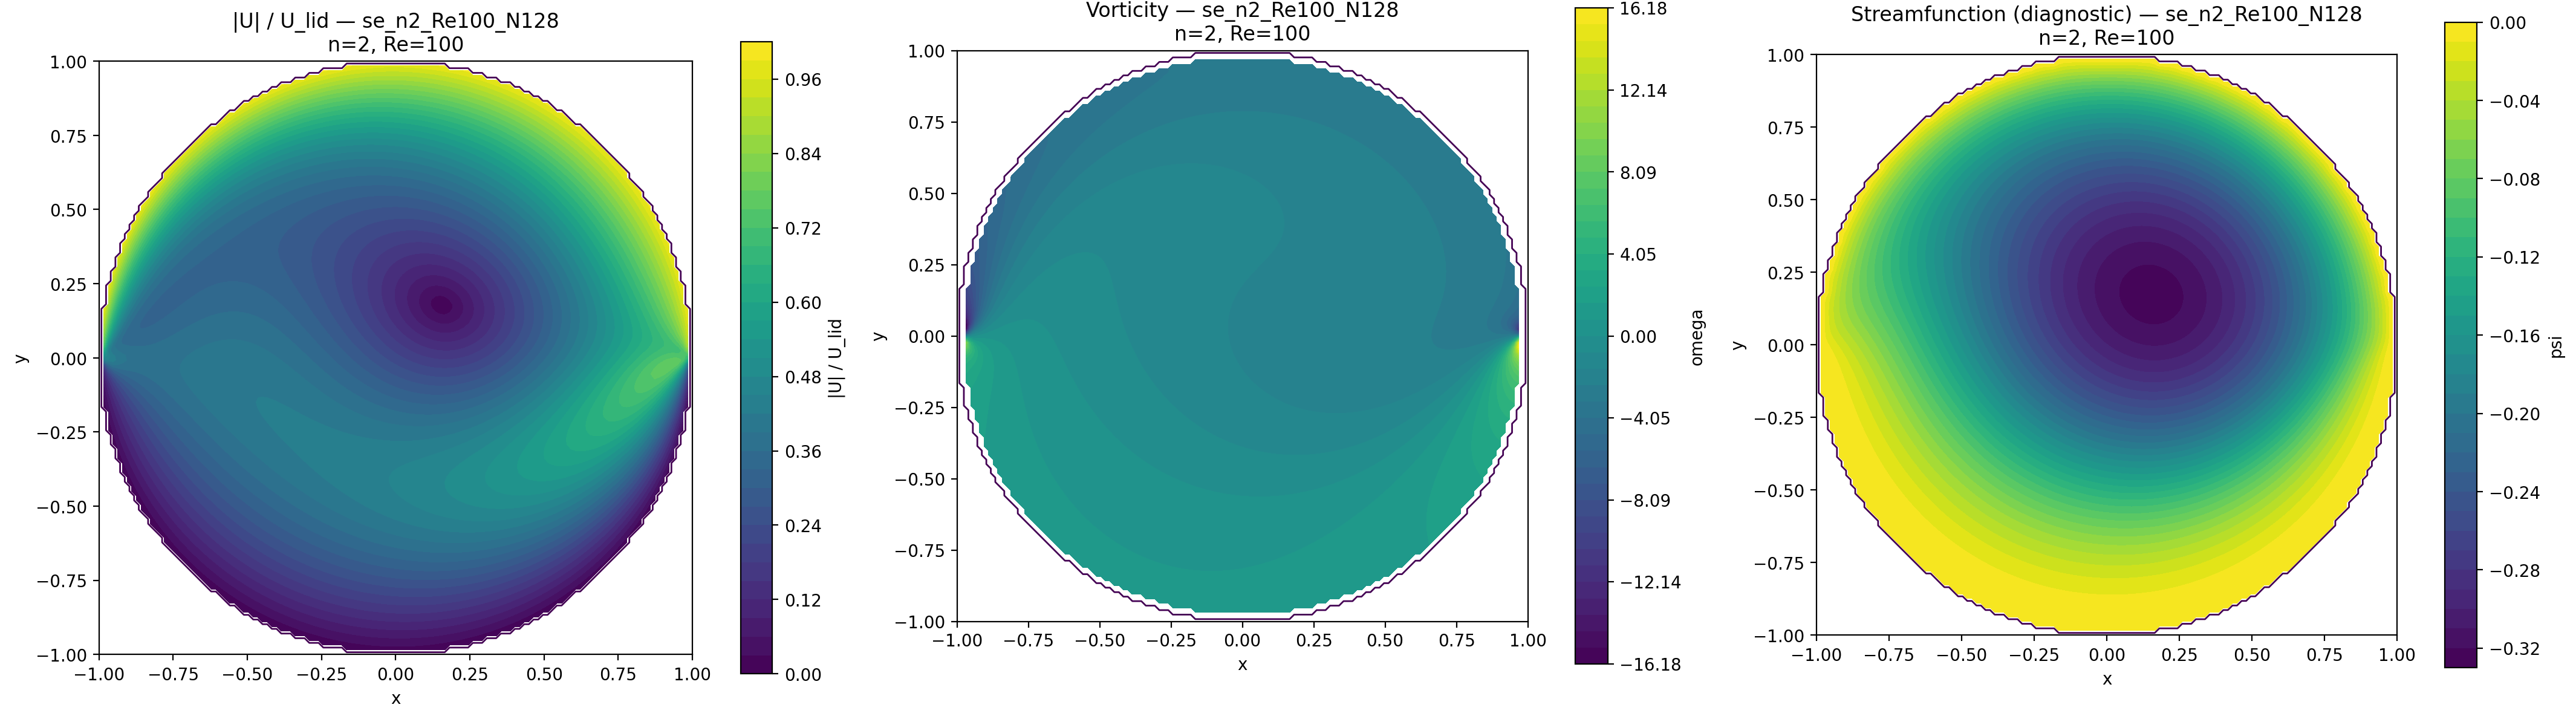
\includegraphics[width=\textwidth]{se_n2p0_Re100_N128_fields.png}
\caption{$n=2,\;Re=100$}
\end{subfigure}
\hfill
\begin{subfigure}[b]{0.32\textwidth}
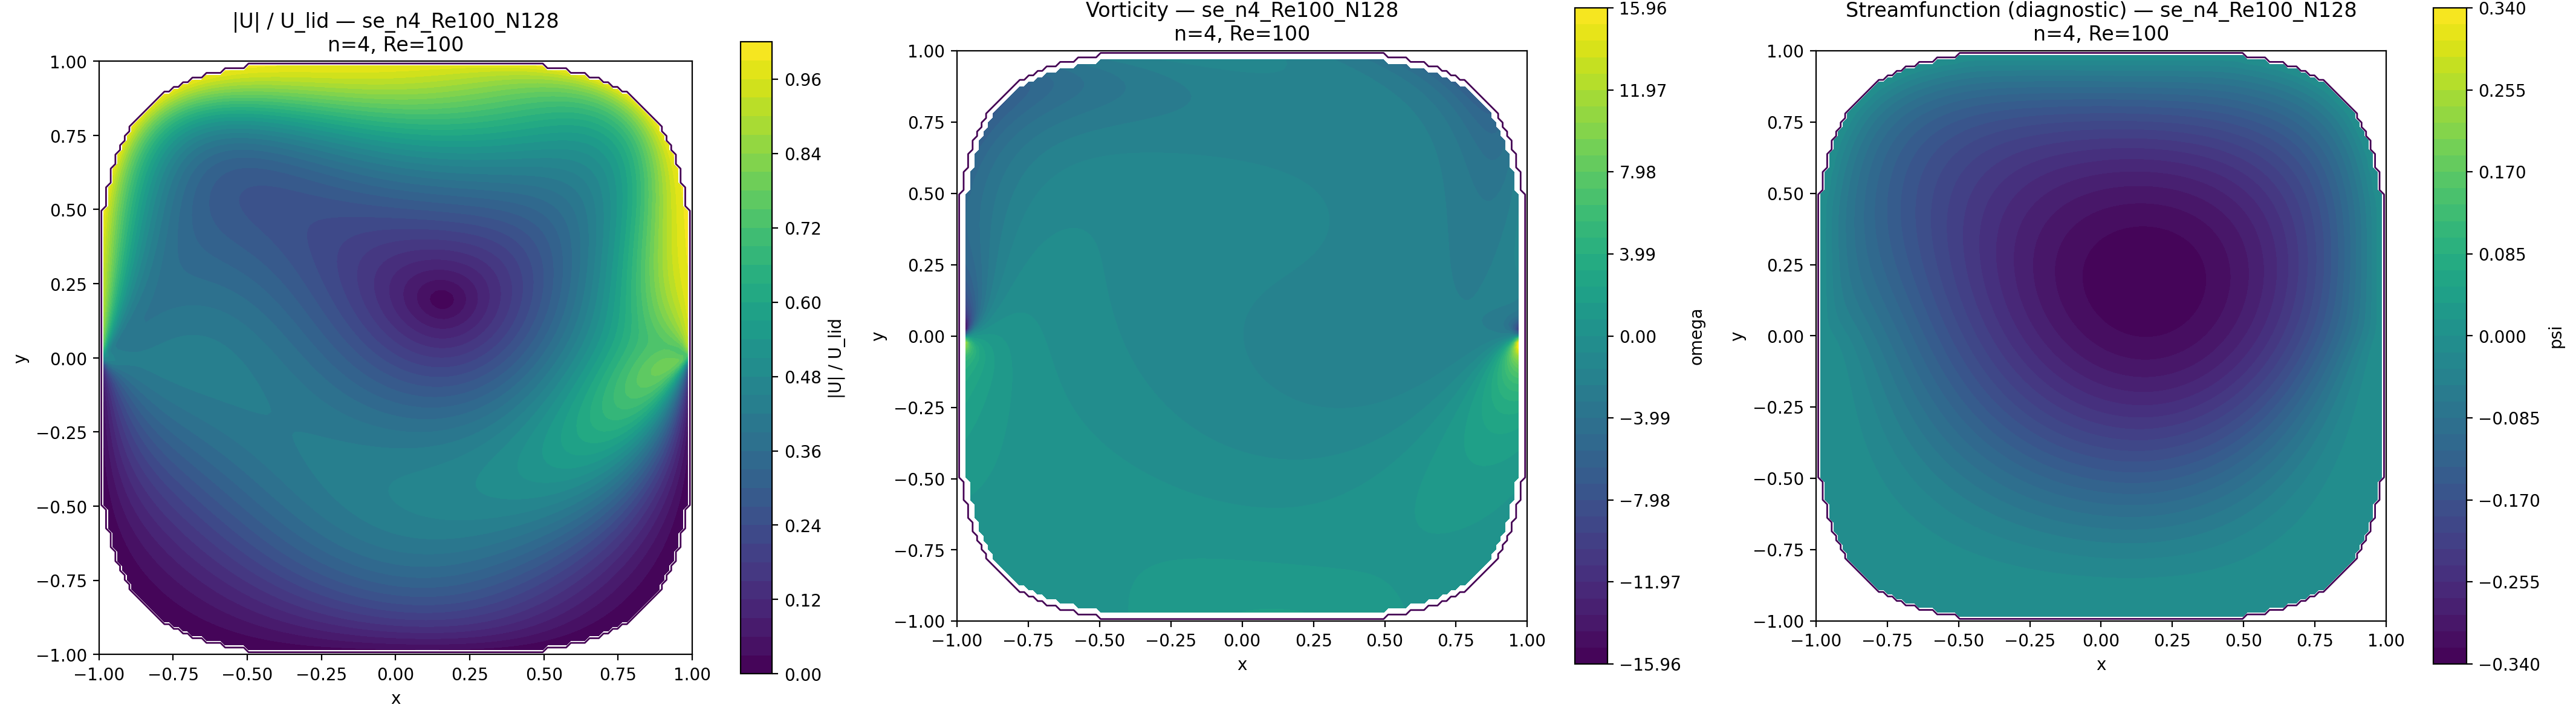
\includegraphics[width=\textwidth]{se_n4p0_Re100_N128_fields.png}
\caption{$n=4,\;Re=100$}
\end{subfigure}
\caption{Reference LBM velocity and streamfunction fields at $Re=100$ for representative geometry exponents.}




\label{fig:atlas100}
\end{figure}



\begin{table}[H]
\centering
\caption{Complete $N=128$ grid of the area-normalized kinetic energy $KE/A$
and area-normalized dissipation $D/A$ in the mechanical convention of
Table~\ref{tab:energy30}. $KE/A$ uses the exact cavity area $A(n)$; $D/A$ uses
the area $A_{\rm mask}(n)$ of the discrete integration mask that carries the
sum defining $D$. Rows are geometry exponents and columns Reynolds numbers.
The absolute levels are resolution-sensitive; the table is used for geometry
ordering at fixed resolution only.}




\label{tab:grid190}
\scriptsize
\setlength{\tabcolsep}{3.0pt}
\tabbox{%
\begin{tabular}{@{}lrrrrrrrrrrrrrrrrrrr@{}}
\toprule
$n$ & 100 & 150 & 200 & 250 & 300 & 350 & 400 & 450 & 500 & 550 & 600 & 650 & 700 & 750 & 800 & 850 & 900 & 950 & 1000 \\
\midrule
\multicolumn{20}{l}{\bfseries $KE/A$}\\
1.25 & 0.0915 & 0.0936 & 0.0951 & 0.0962 & 0.0971 & 0.0978 & 0.0984 & 0.0989 & 0.0993 & 0.0996 & 0.0999 & 0.1002 & 0.1004 & 0.1006 & 0.1008 & 0.1010 & 0.1011 & 0.1013 & 0.1014 \\
1.5 & 0.0994 & 0.1018 & 0.1035 & 0.1047 & 0.1057 & 0.1065 & 0.1071 & 0.1077 & 0.1081 & 0.1086 & 0.1089 & 0.1093 & 0.1096 & 0.1099 & 0.1101 & 0.1104 & 0.1106 & 0.1109 & 0.1111 \\
1.75 & 0.1039 & 0.1064 & 0.1081 & 0.1094 & 0.1104 & 0.1112 & 0.1119 & 0.1125 & 0.1130 & 0.1134 & 0.1139 & 0.1142 & 0.1146 & 0.1149 & 0.1152 & 0.1155 & 0.1158 & 0.1161 & 0.1164 \\
2 & 0.1055 & 0.1080 & 0.1097 & 0.1110 & 0.1120 & 0.1128 & 0.1135 & 0.1141 & 0.1147 & 0.1151 & 0.1156 & 0.1160 & 0.1163 & 0.1167 & 0.1170 & 0.1173 & 0.1176 & 0.1179 & 0.1182 \\
2.5 & 0.1057 & 0.1082 & 0.1099 & 0.1111 & 0.1121 & 0.1129 & 0.1135 & 0.1141 & 0.1146 & 0.1150 & 0.1154 & 0.1158 & 0.1162 & 0.1165 & 0.1168 & 0.1171 & 0.1174 & 0.1176 & 0.1179 \\
3 & 0.1038 & 0.1063 & 0.1080 & 0.1092 & 0.1101 & 0.1109 & 0.1115 & 0.1121 & 0.1126 & 0.1130 & 0.1134 & 0.1138 & 0.1141 & 0.1144 & 0.1147 & 0.1150 & 0.1152 & 0.1155 & 0.1158 \\
4 & 0.1006 & 0.1031 & 0.1048 & 0.1060 & 0.1070 & 0.1077 & 0.1084 & 0.1089 & 0.1094 & 0.1099 & 0.1103 & 0.1107 & 0.1110 & 0.1114 & 0.1117 & 0.1120 & 0.1123 & 0.1126 & 0.1129 \\
5 & 0.0981 & 0.1007 & 0.1025 & 0.1038 & 0.1047 & 0.1055 & 0.1062 & 0.1068 & 0.1073 & 0.1078 & 0.1082 & 0.1086 & 0.1090 & 0.1093 & 0.1097 & 0.1100 & 0.1103 & 0.1106 & 0.1109 \\
6 & 0.0962 & 0.0989 & 0.1007 & 0.1021 & 0.1031 & 0.1039 & 0.1046 & 0.1052 & 0.1057 & 0.1062 & 0.1066 & 0.1070 & 0.1074 & 0.1077 & 0.1081 & 0.1084 & 0.1087 & 0.1090 & 0.1092 \\
8 & 0.0938 & 0.0966 & 0.0985 & 0.0999 & 0.1010 & 0.1019 & 0.1027 & 0.1033 & 0.1039 & 0.1044 & 0.1048 & 0.1052 & 0.1056 & 0.1060 & 0.1063 & 0.1066 & 0.1070 & 0.1072 & 0.1075 \\
\midrule
\multicolumn{20}{l}{\bfseries $D/A$}\\
1.25 & 0.07959 & 0.05743 & 0.04593 & 0.03877 & 0.03382 & 0.03016 & 0.02733 & 0.02507 & 0.02321 & 0.02165 & 0.02032 & 0.01917 & 0.01816 & 0.01727 & 0.01648 & 0.01576 & 0.01512 & 0.01454 & 0.01400 \\
 1.5 & 0.05360 & 0.03988 & 0.03255 & 0.02787 & 0.02458 & 0.02212 & 0.02019 & 0.01862 & 0.01733 & 0.01623 & 0.01529 & 0.01447 & 0.01375 & 0.01311 & 0.01254 & 0.01202 & 0.01155 & 0.01112 & 0.01073 \\
1.75 & 0.04320 & 0.03266 & 0.02692 & 0.02322 & 0.02060 & 0.01861 & 0.01705 & 0.01577 & 0.01471 & 0.01381 & 0.01304 & 0.01236 & 0.01176 & 0.01123 & 0.01075 & 0.01032 & 0.00992 & 0.00957 & 0.00924 \\
   2 & 0.03814 & 0.02903 & 0.02404 & 0.02080 & 0.01848 & 0.01673 & 0.01534 & 0.01421 & 0.01326 & 0.01246 & 0.01177 & 0.01116 & 0.01062 & 0.01014 & 0.00972 & 0.00933 & 0.00897 & 0.00865 & 0.00835 \\
 2.5 & 0.03421 & 0.02613 & 0.02168 & 0.01878 & 0.01671 & 0.01513 & 0.01388 & 0.01286 & 0.01201 & 0.01128 & 0.01066 & 0.01011 & 0.00962 & 0.00919 & 0.00880 & 0.00845 & 0.00813 & 0.00784 & 0.00757 \\
   3 & 0.03335 & 0.02541 & 0.02104 & 0.01820 & 0.01617 & 0.01462 & 0.01340 & 0.01241 & 0.01157 & 0.01087 & 0.01025 & 0.00972 & 0.00925 & 0.00883 & 0.00845 & 0.00811 & 0.00780 & 0.00751 & 0.00725 \\
   4 & 0.03412 & 0.02579 & 0.02124 & 0.01829 & 0.01620 & 0.01461 & 0.01336 & 0.01235 & 0.01150 & 0.01078 & 0.01016 & 0.00962 & 0.00915 & 0.00872 & 0.00834 & 0.00800 & 0.00769 & 0.00740 & 0.00714 \\
   5 & 0.03571 & 0.02678 & 0.02194 & 0.01883 & 0.01663 & 0.01497 & 0.01366 & 0.01260 & 0.01172 & 0.01098 & 0.01033 & 0.00978 & 0.00928 & 0.00885 & 0.00846 & 0.00811 & 0.00779 & 0.00750 & 0.00723 \\
   6 & 0.03739 & 0.02784 & 0.02271 & 0.01942 & 0.01710 & 0.01536 & 0.01400 & 0.01289 & 0.01197 & 0.01120 & 0.01054 & 0.00996 & 0.00945 & 0.00900 & 0.00860 & 0.00823 & 0.00790 & 0.00760 & 0.00733 \\
   8 & 0.04047 & 0.02981 & 0.02414 & 0.02053 & 0.01801 & 0.01612 & 0.01465 & 0.01346 & 0.01248 & 0.01165 & 0.01094 & 0.01033 & 0.00979 & 0.00931 & 0.00888 & 0.00850 & 0.00815 & 0.00784 & 0.00755 \\
\bottomrule
\end{tabular}}
\end{table}


\section{Wall-curvature diagnostic}
\label{sec:curvature}

The wall-curvature diagnostic interpolates the full periodic arclength table,
uses periodic central differences for the tangent angle and a wrapped angular
difference for the window curvature
\begin{equation}
  \kappa_w(s)=\frac{\operatorname{wrap}\left[\phi(s+w/2)-\phi(s-w/2)\right]}{w},
  \qquad w=0.05L_c .
  \label{eq:kappa_window}
\end{equation}
The sharp-set threshold is
$\kappa_w\geq2\langle|\kappa|\rangle_\Gamma$. All $190$ curvature rows were
recomputed from the reference fields; $D$, $A_{\rm mask}$, $D/A_{\rm mask}$ and
the curvature-independent wall-band fractions are unchanged.

\begin{table}[H]
\centering
\caption{Analytical circle test. For $n=2$, $a=b=1$, the boundary is the unit
circle and the exact curvature is $\kappa=1$ everywhere.}




\label{tab:circle}
\tabbox{\begin{tabular}{@{}rrrrr@{}}
\toprule
$n_{\rm samples}$ & $w/L_c$ & $\kappa_{w,\max}$ & $\kappa_{w,\rm rms}$ & $f_{\rm sharp}$ \\
\midrule
2\,000  & 0.01 & 1.000000 & 1.000000 & 0.000 \\
2\,000  & 0.05 & 1.000000 & 1.000000 & 0.000 \\
5\,000  & 0.05 & 1.000000 & 1.000000 & 0.000 \\
20\,000 & 0.05 & 1.000000 & 1.000000 & 0.000 \\
50\,000 & 0.10 & 1.000000 & 1.000000 & 0.000 \\
\bottomrule
\end{tabular}}
\end{table}


\begin{table}[H]
\centering
\caption{Geometry-only curvature metrics (independent of $Re$).}




\label{tab:curvgeom}
\tabbox{\begin{tabular}{@{}crrrr@{}}
\toprule
$n$ & $\kappa_{w,\max}$ & $\kappa_{w,\rm rms}$ & $f_{\rm sharp}$ & $\langle|\kappa|\rangle_\Gamma$ \\
\midrule
1.25 & 8.726 & 2.294 & 0.082 & 1.091 \\
1.50 & 4.394 & 1.393 & 0.084 & 1.058 \\
1.75 & 2.109 & 1.077 & 0.033 & 1.027 \\
2.00 & 1.000 & 1.000 & 0.000 & 1.000 \\
2.50 & 1.397 & 1.023 & 0.000 & 0.960 \\
3.00 & 1.775 & 1.087 & 0.000 & 0.932 \\
4.00 & 2.498 & 1.221 & 0.207 & 0.895 \\
5.00 & 3.192 & 1.345 & 0.215 & 0.873 \\
6.00 & 3.861 & 1.458 & 0.207 & 0.859 \\
8.00 & 5.125 & 1.655 & 0.186 & 0.840 \\
\bottomrule
\end{tabular}}
\end{table}


The maximum curvature is minimal at the circle and rises both at
sharp tips ($n<2$) and near-square corners ($n>2$), as expected geometrically.
The sharp set is empty for $n=2,2.5,3$ and non-empty at both ends of the family.

Let $\phi=2\nu S:S$ denote the dissipation density on the gradient-valid mask
$M$. The dissipation-weighted curvature and near-wall share used below are
\begin{equation}
  \langle\kappa\rangle_D=
  \frac{\int_M\kappa_w\phi\,dA}{\int_M\phi\,dA},
  \qquad
  f_\delta=\frac{\int_{M\cap\{{\rm dist}(x,\Gamma)\le\delta L_c\}}\phi\,dA}
                 {\int_M\phi\,dA},
  \label{eq:curvweighted}
\end{equation}
so $f_{0.025}$ corresponds to $\delta=0.025L_c$.

\begin{table}[H]
\centering
\caption{Correlations with $D/A_{\rm mask}$ at fixed $Re$. Spearman values
are shown only for $Re=1000$.}




\label{tab:currcorr}
\tabbox{\begin{tabular}{@{}lcccc@{}}
\toprule
predictor & $Re=100$, $r$ & $Re=500$, $r$ & $Re=1000$, $r$ & $Re=1000$, $\rho$ \\
\midrule
$\kappa_{w,\rm rms}$ & $+0.834$ & $+0.748$ & $+0.709$ & $+0.115$ \\
$\langle\kappa\rangle_D$ & $+0.667$ & $+0.462$ & $+0.385$ & $+0.636$ \\
$f_{\rm sharp}$ & $+0.794$ & $-0.068$ & $-0.238$ & $-0.472$ \\
$f_{0.025}$ & $+0.795$ & $+0.852$ & $+0.848$ & $+0.794$ \\
\bottomrule
\end{tabular}}
\end{table}


At fixed $Re$, RMS window curvature remains positively correlated with
$D/A_{\rm mask}$, but the Pearson coefficient decreases from $+0.834$ at
$Re=100$ to $+0.709$ at $Re=1000$ and the Spearman coefficient at $Re=1000$
is only $+0.115$. The sharp-set fraction is negatively correlated at $Re=500$
and $Re=1000$. These results do not support wall curvature alone as the
control on the $D/A_{\rm mask}$ minimum.

\begin{figure}[H]
\centering
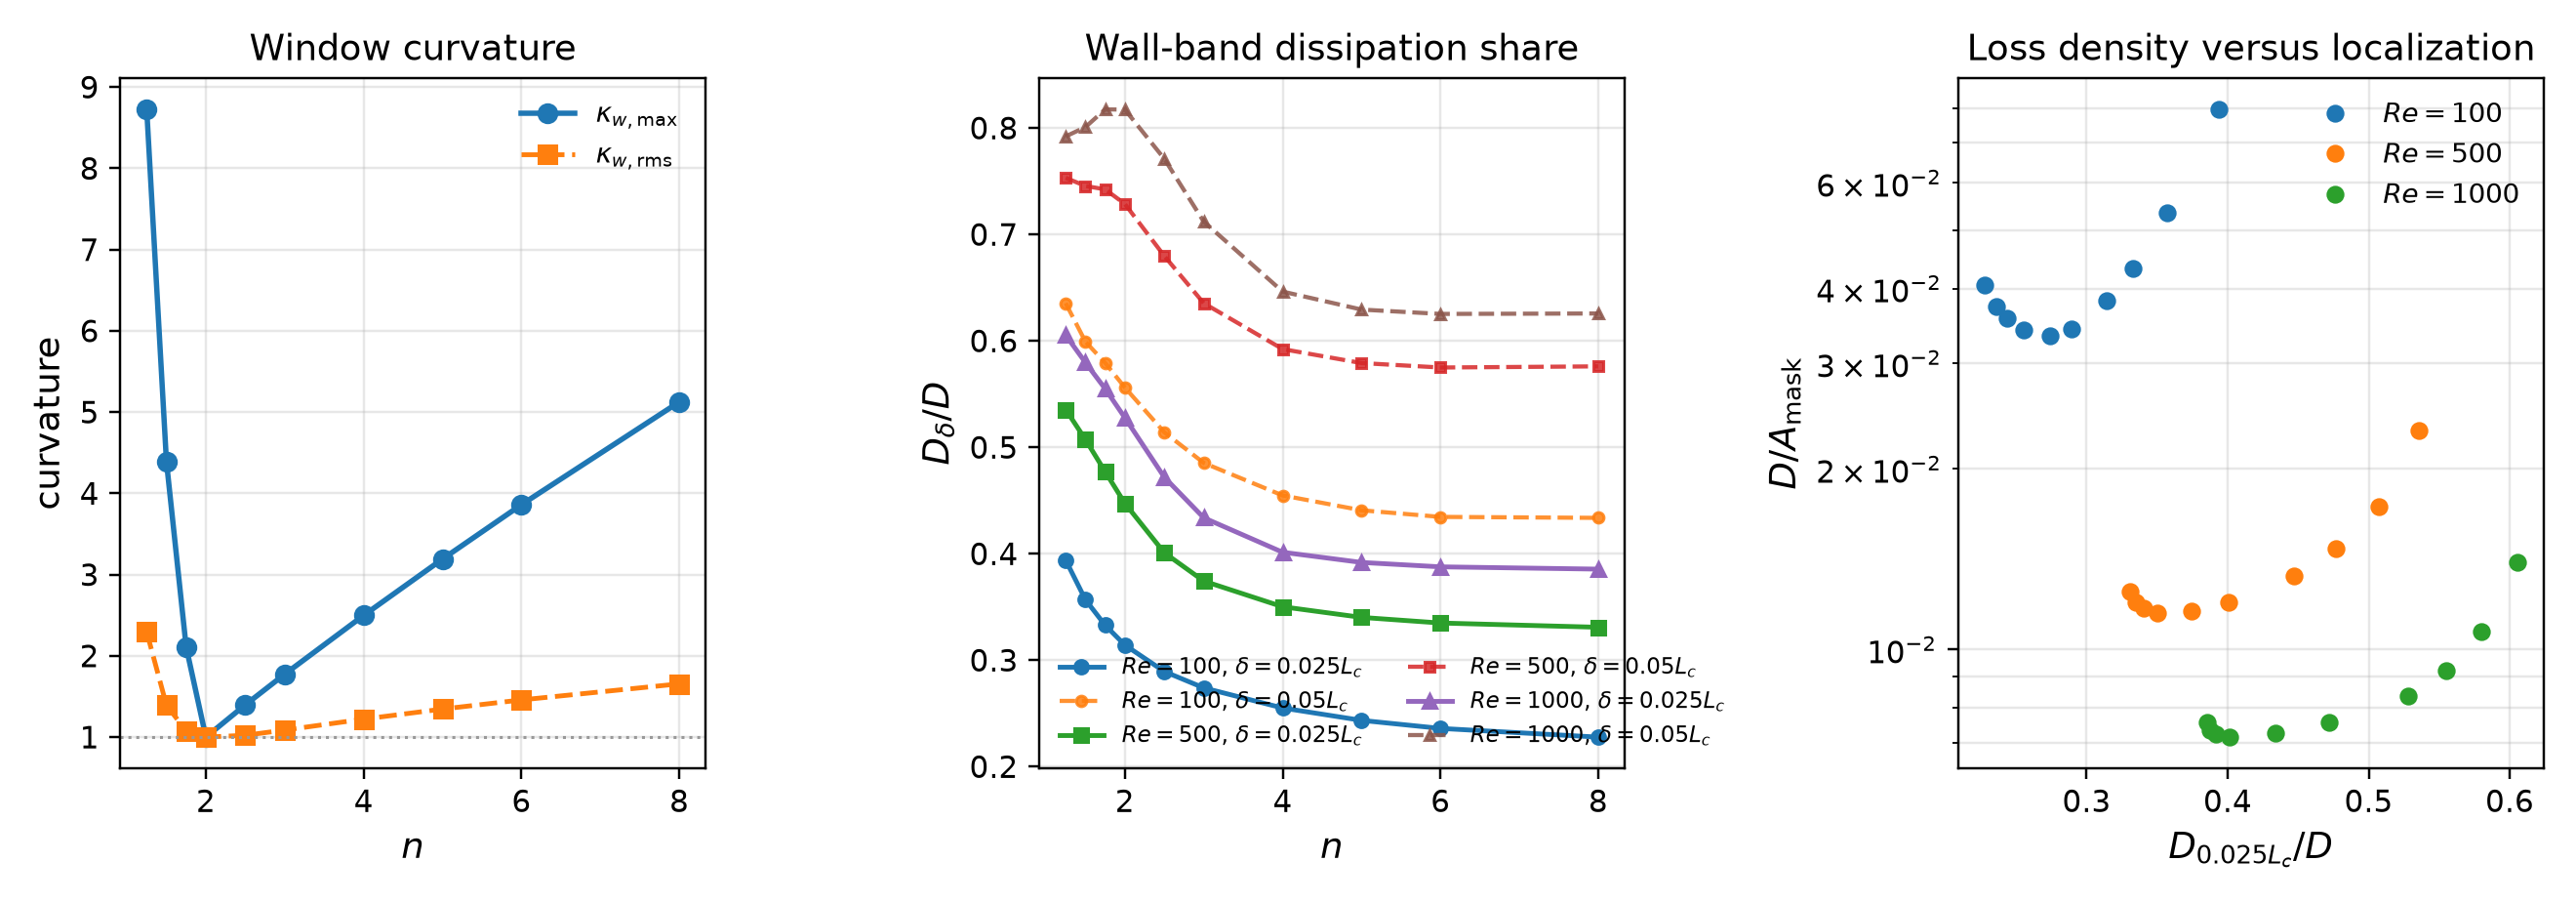
\includegraphics[width=0.96\textwidth]{fig_nearwall_large_axes.png}
\caption{Wall-curvature diagnostic, wall-band dissipation share and
$D/A_{\rm mask}$ versus wall-band localization on the reference grid. Axes and
tick labels are enlarged for clarity; the panels use the periodic
arclength interpolation.}




\label{fig:nearwall_large}
\end{figure}


\section{Extended additive wall/core budget}
\label{sec:corewall}

For every case the same gradient-valid mask $M$ is partitioned into
$W_\delta=M\cap\{\operatorname{dist}(\mathbf{x},\Gamma)\leq\delta\}$ and
$C_\delta=M\setminus W_\delta$, with $\delta/L_c\in\{0.025,0.05\}$. Using the
same integrand as in Eq.~\eqref{eq:mech_factor},
\[
  \frac{D_{\rm mask}}{A_{\rm mask}}
  =\frac{D_{\rm wall}}{A_{\rm mask}}+\frac{D_{\rm core}}{A_{\rm mask}},
  \qquad A_{\rm mask}=N_M\Delta x^2 .
\]
The dataset comprises $253$ cases and two band widths, hence $506$ rows. The
maximum absolute additivity residual over all rows is $2.78\times10^{-17}$.

\begin{table}[H]
\centering
\caption{Additive budget for the detailed case $Re=1000$, $N=256$,
$\delta=0.05L_c$. All denominators are $A_{\rm mask}$, never $A_{\rm core}$
or the exact geometric area.}




\label{tab:budgetcase}
\tabbox{\begin{tabular}{@{}crrrr@{}}
\toprule
$n$ & $D/A_{\rm mask}$ & $D_{\rm wall}/A_{\rm mask}$ & $D_{\rm core}/A_{\rm mask}$ & $f_{\rm core}$ \\
\midrule
2 & 0.010289 & 0.008853 & 0.001437 & 14.0\% \\
3 & 0.008943 & 0.006941 & 0.002002 & 22.4\% \\
4 & 0.008797 & 0.006329 & 0.002468 & 28.1\% \\
6 & 0.008968 & 0.006235 & 0.002733 & 30.5\% \\
8 & 0.009199 & 0.006378 & 0.002821 & 30.7\% \\
\bottomrule
\end{tabular}
}
\end{table}


\begin{figure}[H]
\centering
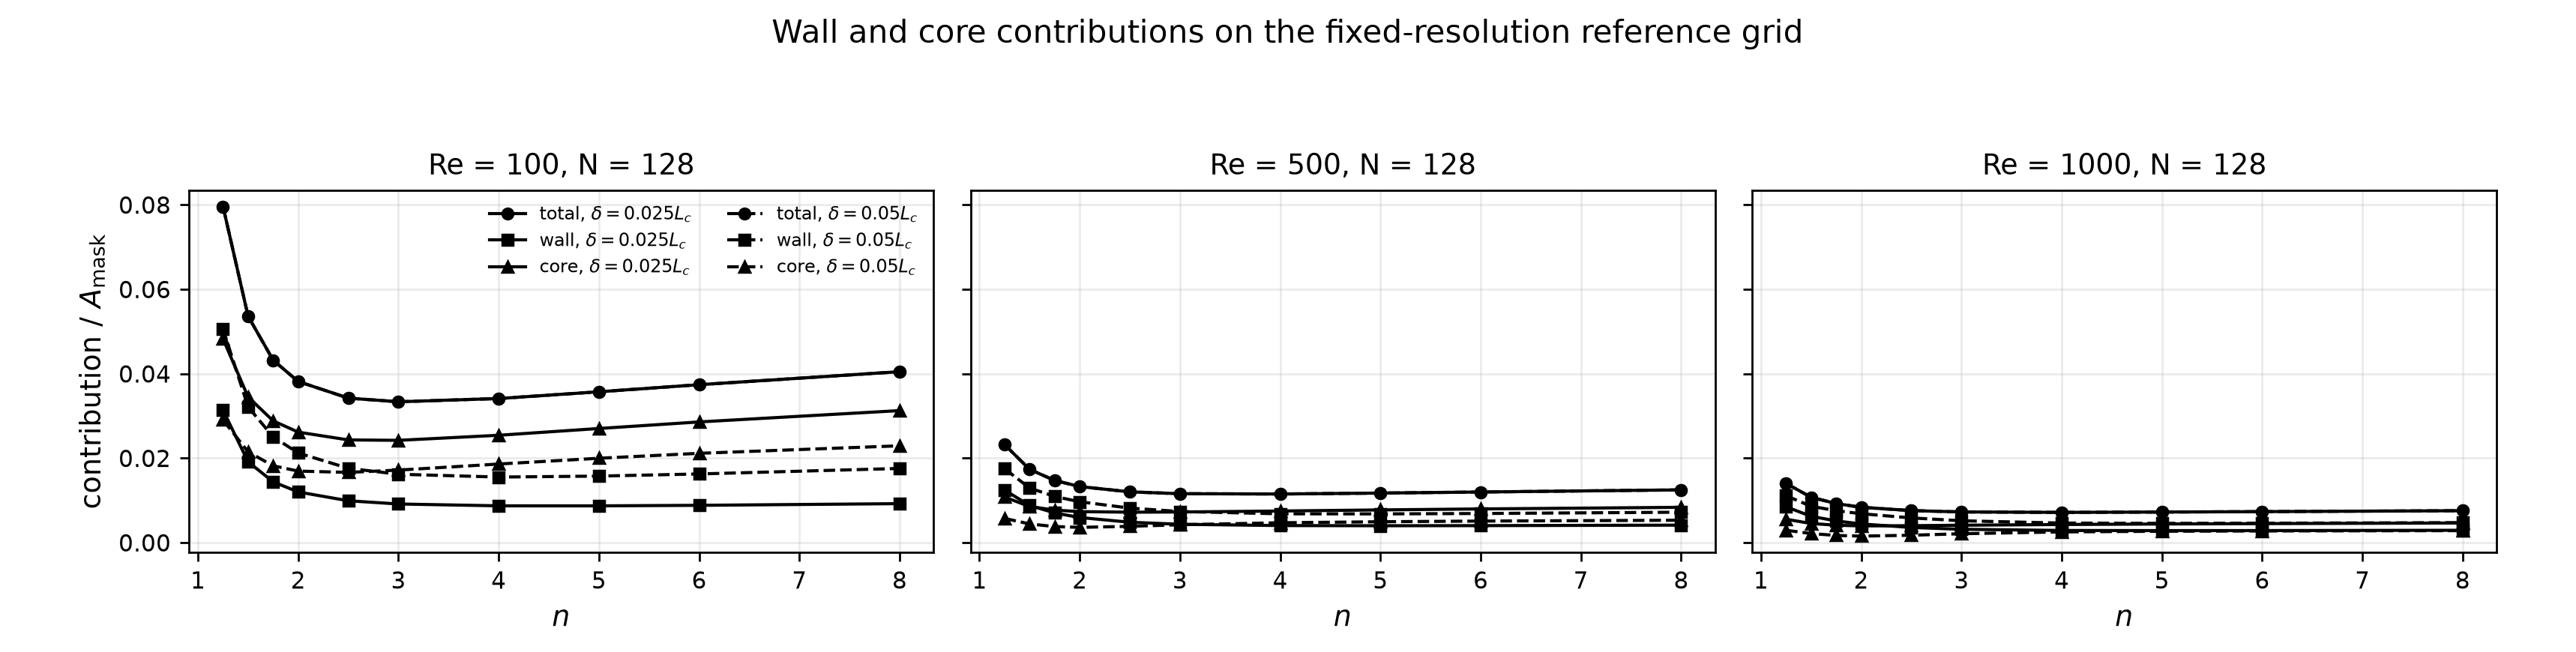
\includegraphics[width=0.94\textwidth]{fig_supp_corewall_Re100_500_1000.png}
\caption{Total, wall and core contributions divided by $A_{\rm mask}$ for
$N=128$, $Re=100,500,1000$. Solid lines use $\delta=0.025L_c$ and dashed
lines use $\delta=0.05L_c$.}




\label{fig:corewall}
\end{figure}


Table~\ref{tab:budgetcase} gives the detailed target case. From $n=4$ to
$n=8$, $D/A_{\rm mask}$ rises by $0.000402$, of which $0.000353$ ($87.8\%$) is
the core contribution and $0.000049$ ($12.2\%$) is the wall contribution. The
$88\%$ number is the core share of the \emph{increase}, not the core share of the
total dissipation. The latter is $28.1\%$ at $n=4$ and $30.7\%$ at $n=8$.
Increments in this paragraph and in Table~\ref{tab:budgetrange} are rounded to
six decimals; the percentages are computed from the unrounded fields.

\begin{table}[H]
\centering
\caption{Core share of the $n=4\to8$ increase wherever both exponents exist.
The $Re=100$, $N=256$ increment is unavailable because that campaign has no
$n=8$ field.}




\label{tab:budgetrange}
\tabbox{\begin{tabular}{@{}ccrrrr@{}}
\toprule
$N$ & $Re$ & $\delta/L_c$ & $\Delta(D/A)$ & $\Delta(D_{\rm core}/A)$ & core share \\
\midrule
128 & 100 & 0.025 & 0.006356 & 0.005841 & 91.9\% \\
128 & 100 & 0.05 & 0.006356 & 0.004319 & 67.9\% \\
128 & 500 & 0.025 & 0.000978 & 0.000876 & 89.6\% \\
128 & 500 & 0.05 & 0.000978 & 0.000601 & 61.5\% \\
128 & 1000 & 0.025 & 0.000404 & 0.000361 & 89.5\% \\
128 & 1000 & 0.05 & 0.000404 & 0.000298 & 73.8\% \\
256 & 500 & 0.025 & 0.000992 & 0.000921 & 92.9\% \\
256 & 500 & 0.05 & 0.000992 & 0.000657 & 66.3\% \\
256 & 1000 & 0.025 & 0.000402 & 0.000402 & 99.8\% \\
256 & 1000 & 0.05 & 0.000402 & 0.000353 & 87.8\% \\
\bottomrule
\end{tabular}
}
\end{table}


Table~\ref{tab:budgetrange} qualifies the generalization. Across the ten
available $(N,Re,\delta)$ combinations the core share of the positive increment
lies between $61.5\%$ and $99.8\%$. The share depends on resolution, Reynolds
number and band thickness; no universal causal percentage is claimed. The
underlying $n$ grids are not uniform across campaigns, so comparisons are made
only where the same two exponents are present.

\section{Common-support LBM/FEM dissipation}
\label{sec:common_support}

The computed LBM fields store velocities normalized by the lattice lid speed
$U_{\rm lid}^{\rm lbm}=0.05$ and are expressed on coordinates $x,y\in[-1,1]$
with $a=1$ and $L_c=2$. In the paper convention used below the lid speed is
unity and the viscosity is $\nu=U_{\rm lid}L_c/Re=2/Re$. The LBM integrand used throughout the physics article is
\begin{equation}
  2\nu\,S:S = 2\nu\left(u_x^2+v_y^2+\tfrac12(u_y+v_x)^2\right)
            = \frac{2}{Re}\left(2u_x^2+2v_y^2+(u_y+v_x)^2\right),
  \label{eq:mech_factor}
\end{equation}
so the mechanical factor two in $D=2\int(2S:S/Re)\,dA$ is counted once. The
FEM form assembled from the P2 degrees of freedom is
$D_{\rm FEM}^{\Omega}=2\nu\int_\Omega S(\mathbf{u}_h):S(\mathbf{u}_h)\,dA$
with $U_{\rm lid}=1$ and the same $\nu=2/Re$. No additional velocity rescaling
or second factor two is applied.

The LBM value $D_{\rm LBM}^{M}$ uses central differences on the gradient-valid
mask $M$:
\begin{equation}
  M=\{\mathbf{x}_{jk}\in\Omega_{\rm fluid}^{\rm grid}:\;
      \mathbf{x}_{jk\pm1}\in\Omega_{\rm fluid}^{\rm grid}
      \text{ in both coordinate directions}\},
  \qquad
  D_{\rm LBM}^{M}=2\nu\sum_{k\in M}S_{k}:S_{k}\,\Delta x^2 .
  \label{eq:mask}
\end{equation}
For the same-support FEM value, each $k\in M$ is projected onto its containing
P2 element, the strain is evaluated from the element shape functions, and the
same lattice weight $\Delta x^2$ is used:
$D_{\rm FEM}^{M}=2\nu\sum_{k\in M}S_h(\mathbf{x}_k):S_h(\mathbf{x}_k)\Delta x^2$.
All $9\,488$--$15\,168$ masked nodes were covered by the $n_{\rm ref}=6$ mesh.

\begin{table}[H]
\centering
\caption{Common-support dissipation at $N=128$ and $n_{\rm ref}=6$.
Here $\varepsilon_D=100|D_{\rm LBM}^{M}-D_{\rm FEM}^{M}|/D_{\rm FEM}^{M}$;
the last column is the same FEM strain integrated over the full P2 domain.}




\label{tab:commonsupport}
\tabbox{\begin{tabular}{@{}ccrrrr@{}}
\toprule
$n$ & $Re$ & $D_{\rm LBM}^{M}$ & $D_{\rm FEM}^{M}$ & $\varepsilon_D$ (\%) & $D_{\rm FEM}^{\Omega}$ \\
\midrule
1.25 & 100 & 0.211656 & 0.200336 & 5.65 & 0.327424 \\
1.25 & 1000 & 0.035837 & 0.032877 & 9.00 & 0.062231 \\
2 & 100 & 0.117331 & 0.116496 & 0.72 & 0.224821 \\
2 & 1000 & 0.022538 & 0.024512 & 8.05 & 0.049404 \\
4 & 100 & 0.107158 & 0.121964 & 12.14 & 0.233612 \\
4 & 1000 & 0.020330 & 0.024620 & 17.42 & 0.050635 \\
8 & 100 & 0.127297 & 0.152335 & 16.44 & 0.267256 \\
8 & 1000 & 0.022126 & 0.027665 & 20.02 & 0.054848 \\
\bottomrule
\end{tabular}
}
\end{table}


\begin{figure}[H]
\centering
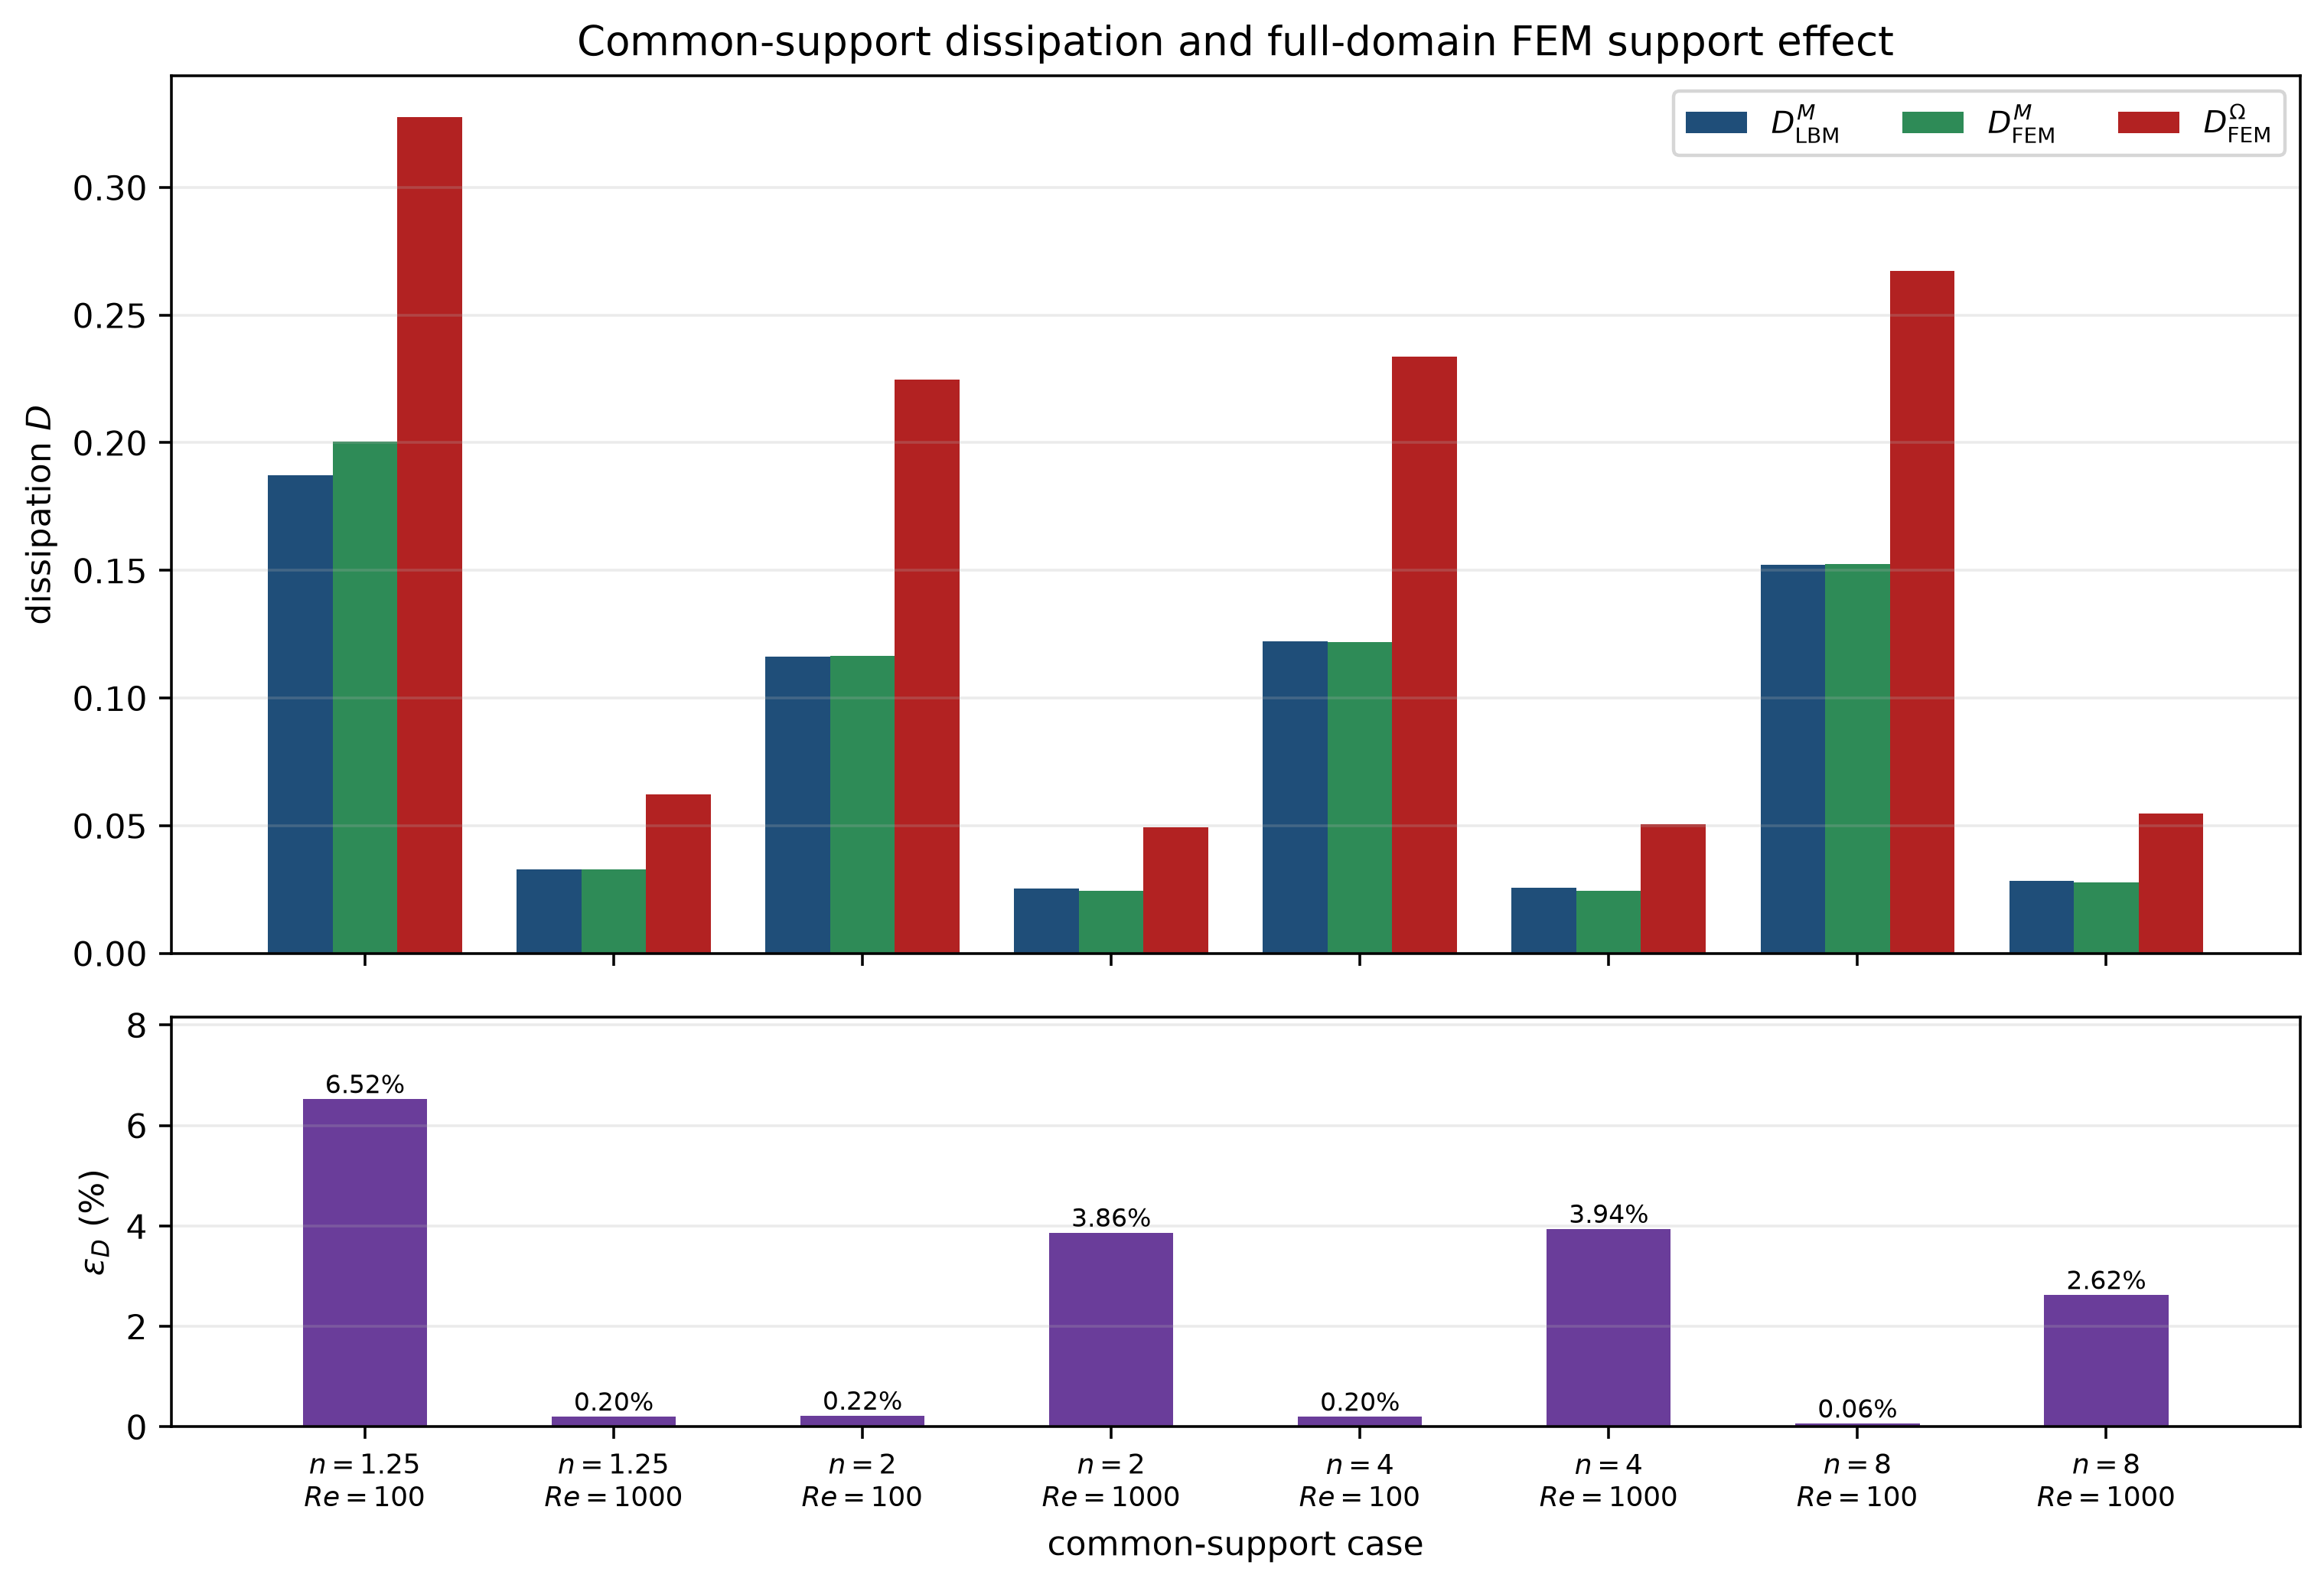
\includegraphics[width=0.88\textwidth]{fig_supp_common_support_dissipation.png}
\caption{Comparison of $D_{\rm LBM}^{M}$, $D_{\rm FEM}^{M}$ and
$D_{\rm FEM}^{\Omega}$ for the eight common-support cases. The difference
between the two FEM bars is a support effect, not a different velocity
normalization.}




\label{fig:commonsupport}
\end{figure}


Table~\ref{tab:commonsupport} and Fig.~\ref{fig:commonsupport} show the
corrected range $\varepsilon_D=0.06$--$6.52\%$, while
$D_{\rm FEM}^{\Omega}/D_{\rm FEM}^{M}=1.63$--$2.06$. The full-domain FEM
integral therefore contains about $39$--$52\%$ more dissipation than the
common-support value, so the layer omitted by $M$ carries approximately
$39$--$52\%$ of $D_{\rm FEM}^{\Omega}$; this is a support mismatch, not
LBM/FEM disagreement on the sampled mask. A fixed-physical-support comparison
at $r_0>0$, $N=128$/$256$ and $n_{\mathrm{ref}}=6/7$ was not run, so the omitted
layer is not resolved across meshes here. Both solvers use the same
$D=2\nu\int S:S\,dA$ convention. For $n=4$, $Re=1000$,
$D_{\rm LBM}^{M}=0.02558962$, $D_{\rm FEM}^{M}=0.02461972$ and
$\varepsilon_D=3.94\%$. The quantity labelled
``rel.\ $D$ error'' in the gradient-reconstruction table is
$|D_{\rm FD,lattice}-D_{\rm exact,lattice}|/D_{\rm exact,lattice}$: it compares
two gradient reconstructions at lattice points sampled from a saved FEM field,
and is not an LBM/FEM validation error. The closest common-support agreement
occurs at $n=8$, $Re=100$; the largest discrepancy occurs at $n=1.25$,
$Re=100$. These values are a same-support comparison, not a grid-converged
absolute validation or a verified lid-power balance.

\section{FEM mesh, iteration and junction budget}
\label{sec:fem_budget}

The independent solver is a Taylor--Hood P2/P1 Navier--Stokes implementation.
The saddled system is assembled with $\nu=U_{\rm lid}L_c/Re$ and solved by
Picard iteration with relaxation $1$ and a relative $L_2$ velocity tolerance
$10^{-9}$. The verification ladder used $U_{\rm lid}=1$, $a=1$,
$\nu=2/Re$, quadrature order $4$, $n\in\{1.25,2,4,8\}$,
$Re\in\{100,400,1000\}$ and $n_{\rm ref}\in\{4,5,6\}$: $12$ cases and $36$
solves. All $36$ solves converged in $14$--$34$ iterations.

\begin{table}[H]
\centering
\caption{Taylor--Hood mesh levels used in the verification ladder. The total
unknown count is $2(V+E)+V$: vector P2 velocity plus scalar P1 pressure.}




\label{tab:femmesh}
\tabbox{\begin{tabular}{@{}rrrrr@{}}
\toprule
$n_{\rm ref}$ & vertices $V$ & triangles $T$ & velocity DOFs & total unknowns \\
\midrule
4 & 545  & 1\,024  & 4\,226  & 4\,771  \\
5 & 2\,113 & 4\,096  & 16\,642 & 18\,755 \\
6 & 8\,321 & 16\,384 & 66\,050 & 74\,371 \\
\bottomrule
\end{tabular}}
\end{table}


The Dirichlet assignment is nodal and discontinuous. For every boundary
velocity degree of freedom, the FEM code evaluates $y>0$ and imposes
$U_{\rm lid}(m_y,-m_x)$ if true and $\mathbf{0}$ otherwise; there is no
interpolation or regularization length. The same strict label is used for LBM
boundary links. The radial mesh retains cardinal nodes at $(\pm1,0)$ to
machine precision. A runtime check on the executed meshes gives:

\begin{itemize}
  \item right junction $(+1,0)$: $y=0$ exactly, assigned to the fixed wall;
  \item left junction $(-1,0)$: $y=+1.22\times10^{-16}$, assigned to the
        moving wall by the strict $y>0$ test.
\end{itemize}

\begin{figure}[H]
\centering
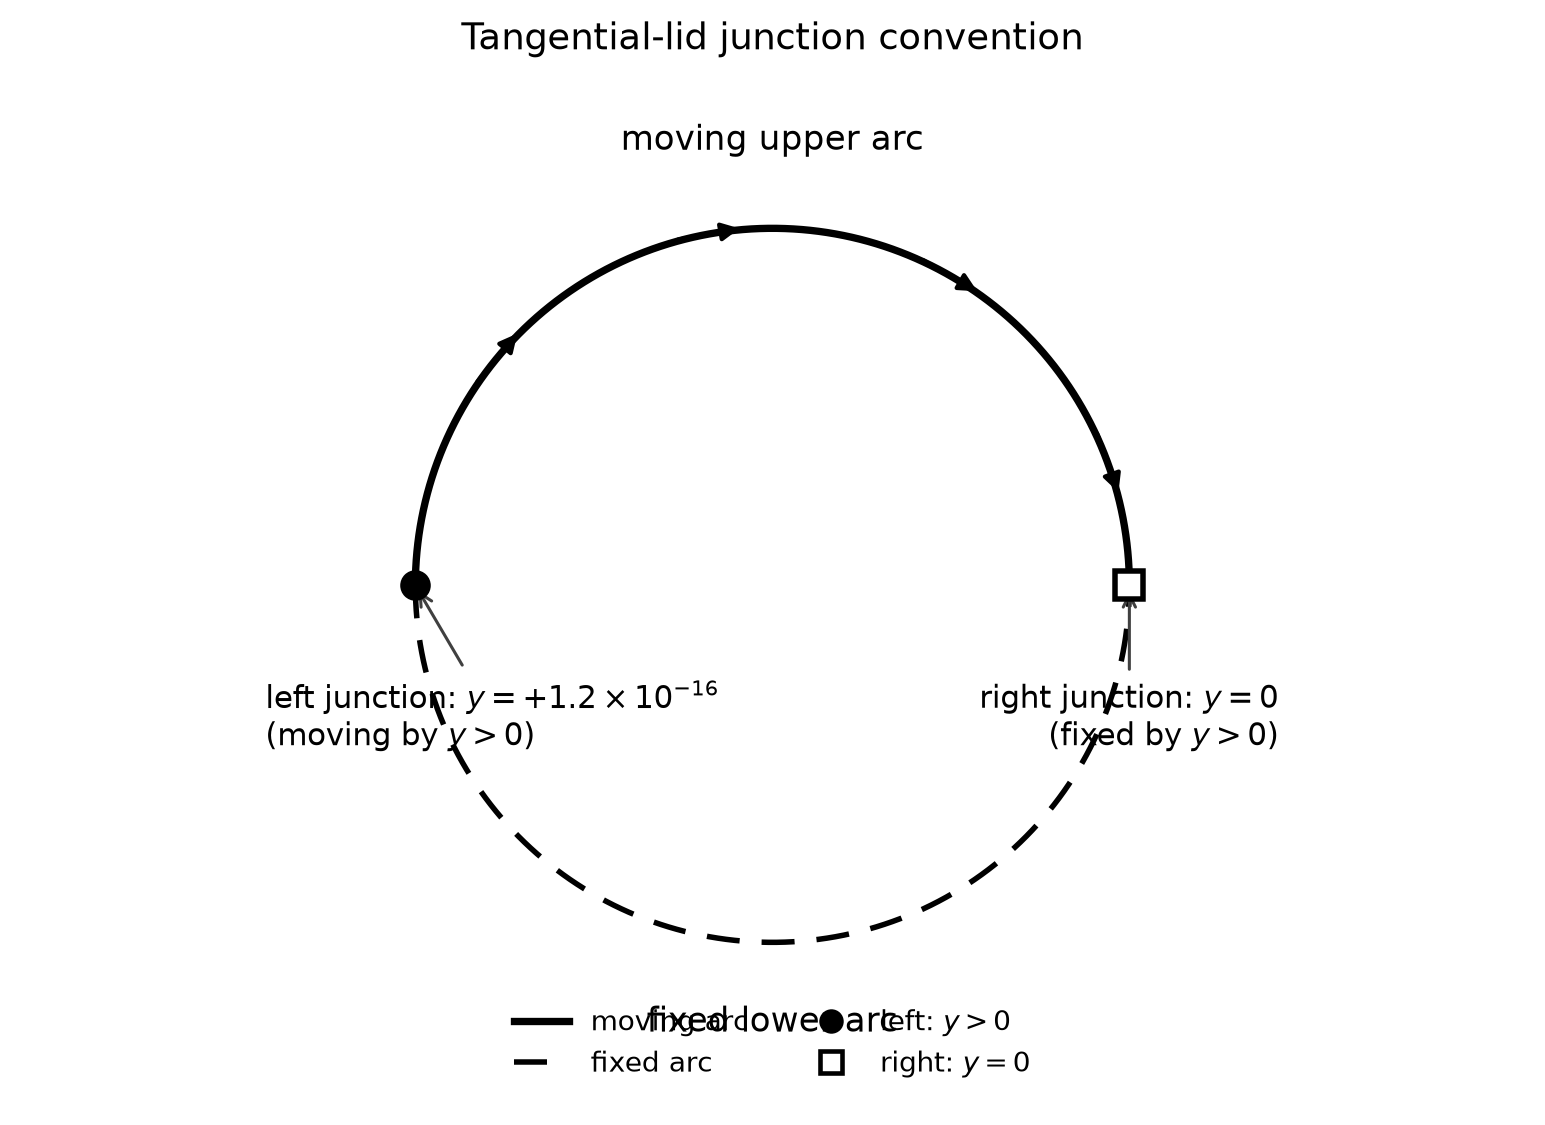
\includegraphics[width=0.72\textwidth]{fig_supp_fem_junction_schematic.png}
\caption{Tangential-lid junction convention. The upper arc is moving and the
lower arc is fixed. The two junctions are points of velocity discontinuity;
the FEM assignment is by a strict nodal $y>0$ test, without blending.}




\label{fig:femjunction_supp}
\end{figure}


This machine-precision asymmetry (Fig.~\ref{fig:femjunction_supp}) is a
discrete implementation detail, not a physical regularization. The FEM junction
contribution is therefore mesh-sensitive in the same way as the LBM junction
diagnostic. Direct 5-to-6 mesh changes in $D_{\rm FEM}$ are $1.32\%$--$8.46\%$;
they are reported as mesh sensitivity only, with no Richardson extrapolation.

\subsection{Fixed junction-disk radii and descriptive logarithmic fits}
\label{sec:juncut}

The first cutoff test used disk radii proportional to the lattice spacing, so
it could not distinguish a fixed physical exclusion from a refinement effect.
We therefore recomputed the comparison on thirty matched cases with a fixed
junction-disk radius
$r_0\in\{0,0.125,0.25,0.5\}$ measured in the paper coordinates
$x,y\in[-1,1]$ ($L_c=2$). The two junction disks are excluded from the
gradient-valid mask $M$:
\begin{equation}
  M_{r_0}=M\setminus\bigcup_{x_j=\pm1}B\bigl((x_j,0),r_0\bigr),
  \label{eq:junction_mask_supp}
\end{equation}
and $D_{r_0}(N)=2\nu\sum_{k\in M_{r_0}}S:S\,dx^2$. Table~\ref{tab:juncut}
reports the median and the minimum/maximum of $D_{256}/D_{128}-1$ over the
thirty cases. The median falls
from $21.37\%$ at $r_0=0$ to $8.77\%$ at $r_0=0.5$; the largest-cutoff range is
$4.33$--$14.28\%$. This is a reduction of the measured refinement difference,
not a demonstration of grid-independent continuum dissipation.

\begin{table}[H]
\centering
\caption{Thirty-case refinement difference $D_{256}/D_{128}-1$ with a fixed
physical wall cutoff $r_0$.}
\label{tab:juncut}
\tabbox{\begin{tabular}{@{}lrrr@{}}
\toprule
$r_0$ & median (\%) & min (\%) & max (\%) \\
\midrule
0 & 21.37 & 18.08 & 28.15 \\
0.125 & 12.94 & 8.43 & 21.33 \\
0.25 & 10.14 & 6.62 & 15.82 \\
0.5 & 8.77 & 4.33 & 14.28 \\
\bottomrule
\end{tabular}
}
\end{table}


The available fixed-cutoff ladder for the representative pointed case
$n=8$, $Re=1000$ is recorded in Table~\ref{tab:dr0ladder}, now including the
archived $N=384$ field. For $r_0=0.5$, $D_{r_0}(N)=0.01397$, $0.01824$,
$0.02085$, $0.02189$ and $0.02236$ at $N=64$, $128$, $256$, $384$ and $512$.
The equal-doubling increments are $4277$, $2606$ and $1511$ in units of
$10^{-6}$, with successive ratios $0.609$ and $0.580$. The corresponding
observed orders $p=\log_2(\Delta_{\rm coarse}/\Delta_{\rm fine})$ are $0.71$
and $0.79$: convergence is slow, but it is real on this fixed-radius support.
A Richardson limit using the last doublings is $D_{r_0=0.5,\infty}\simeq
0.0244$, so the $N=512$ value remains about $8.5\%$ below it. The $r_0=0.25$
series behaves similarly ($p\simeq0.61$, $0.80$; limit $\simeq0.0313$;
$N=512$ about $8.8\%$ below), while $r_0=0.125$ gives $p\simeq0.38$, $0.74$.
At $r_0=0$ the equal-doubling ratios are only $0.904$ and $0.846$
($p\simeq0.15$, $0.24$), consistent with logarithmic growth and no finite
Richardson limit. Table~\ref{tab:dr0order} lists the increments and orders;
both tables report diagnostics on the archived ladder, not continuum
certification.

The junction contribution $D_{\rm junction}(r,N)$ was also evaluated on
artificial disks of radius $r=4h,8h,16h$, and the three-grid values were
fitted by $D(N)=a+b\ln N$. Figure~\ref{fig:juncut} panel (b) plots the same
contribution against $\ln(r/h)$ for representative cases; panel (c) shows the
fits and Table~\ref{tab:logfit} lists $a$, $b$ and $R^2$ for the total and
$r=16h$ supports. The latter is not a fixed physical $r_0=0.5$ cutoff:
$16h\simeq0.508$, $0.252$ and $0.125$ at $N=64,128,256$, respectively. The
three-point coefficients imply roughly $+18.7\%$ ($n=3$) and $+19.8\%$ ($n=8$)
from $N=128$ to $N=256$ at $Re=1000$. These values correspond to the
grid-scaled $D_{\rm excl,16h}$ series, not to the fixed-physical $r_0=0.5$
series in Table~\ref{tab:juncut}; they follow the shrinking excluded disk
($0.252\to0.125$) and are not directly comparable with the fixed-cutoff maximum
of $14.28\%$. The high $R^2$ values are
descriptive of the three available grids. They do not establish an asymptotic
logarithmic law, and the fixed physical cutoff does not remove the cutoff
dependence of the full-domain quantity.

\begin{table}[H]
\centering
\caption{Descriptive fits $D(N)=a+b\ln N$ on the $N=64,128,256$ ladder.
The ``total'' support includes the near-junction cells; the $r=16h$ support
excludes them. The latter is grid-scaled, not a fixed physical $r_0=0.5$.}
\label{tab:logfit}
\tabbox{\begin{tabular}{@{}llrrr@{}}
\toprule
case & support & $a$ & $b$ & $R^2$ \\
\midrule
$n=1.25, Re=300$ & total & -0.055985 & 0.027544 & 0.9925 \\
$n=1.25, Re=300$ & $r_0=0.5$ & 0.003932 & 0.009774 & 0.9768 \\
$n=3, Re=1000$ & total & -0.021413 & 0.009489 & 0.9994 \\
$n=3, Re=1000$ & $r_0=0.5$ & -0.005659 & 0.004972 & 0.9785 \\
$n=8, Re=1000$ & total & -0.022881 & 0.010516 & 0.9991 \\
$n=8, Re=1000$ & $r_0=0.5$ & -0.008571 & 0.006369 & 0.9850 \\
\bottomrule
\end{tabular}
}
\end{table}


\begin{figure}[H]
\centering
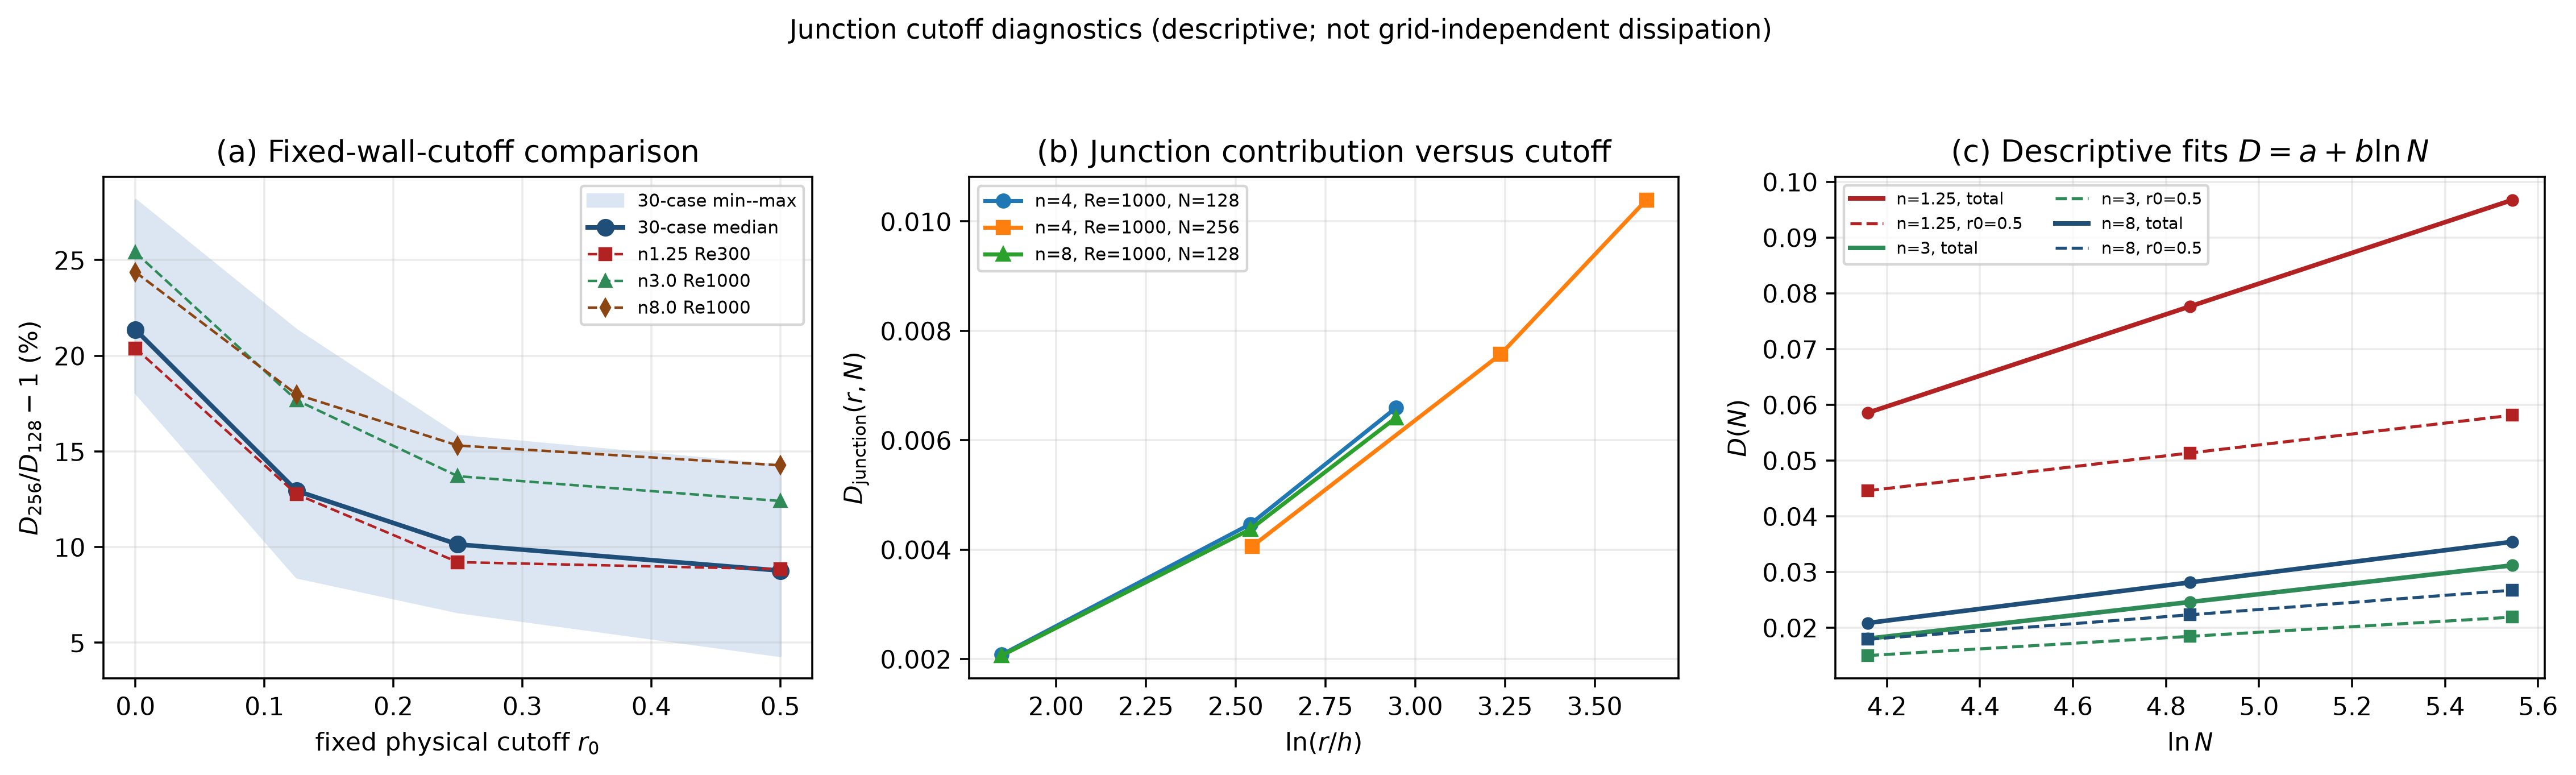
\includegraphics[width=0.98\textwidth]{fig_junction_cutoffs.png}
\caption{(a) Thirty-case fixed-wall-cutoff refinement comparison.
(b) $D_{\rm junction}(r,N)$ versus $\ln(r/h)$.
(c) Descriptive $D(N)=a+b\ln N$ fits on the three-grid ladder; the
excluded support is $r=16h$, not a fixed physical $r_0=0.5$. None of the panels
establishes converged continuum dissipation or asymptotic log scaling.}
\label{fig:juncut}
\end{figure}


\section{Energy identity, pressure convention and field-data diagnostic}
\label{sec:energy}

Three distinct statements must not be confused.

\begin{enumerate}
  \item \emph{Continuous identity.} For a smooth incompressible Newtonian
        velocity and pressure,
        \[
          \nabla\cdot\left[\left(\tfrac12|\mathbf{u}|^2+p\right)\mathbf{u}
          -2\nu S\mathbf{u}\right]=-2\nu S:S .
        \]
        This is an analytical statement and is not what the discrete-field diagnostic
        verifies.
  \item \emph{Exact discrete LBM balance.} The collision--streaming scheme has
        its own discrete momentum and energy bookkeeping. That exact discrete
        balance was not reconstructed from the saved macroscopic fields.
  \item \emph{Field-data diagnostic.} Central differences were applied to the
        computed $(\rho,\mathbf{u})$ pair on the gradient-valid mask, with
        pressure and interface fluxes evaluated on artificial circular cuts.
        This is the only quantity tested here, and it does not close.
\end{enumerate}

For the LBM fields the pressure convention is
$p_{\rm LBM}=c_s^2(\rho_{\rm LBM}-1)$ with $c_s^2=1/3$. Since the stored
velocities are lid-normalized with $U_{\rm lid}=0.05$, the pressure entering
the paper-unit diagnostic is
$p=(\rho-1)/(3U_{\rm lid}^2)$. For $n=4$, $Re=1000$, the diagnostic gives
\begin{equation}
  \frac{\int_{\partial\Omega_{\rm art}}
        \left[(\tfrac12|\mathbf{u}|^2+p)\mathbf{u}-2\nu S\mathbf{u}\right]\cdot\mathbf{n}\,ds}
       {-\int_{\Omega_{\rm exc}}2\nu S:S\,dA}
  =-4.419 ,
  \label{eq:flux_ratio}
\end{equation}
instead of $+1$. Equivalently, the pressure coefficient needed to close the
diagnostic flux is $-0.0783$ instead of $+1$. The likely contributors are
the weakly compressible LBM pressure field, finite-difference gradients on a
near-wall mask and interpolation on the artificial cuts. No empirical pressure
rescaling is applied. No global power-balance closure is claimed, and the
interface flux is retained only as an unverified diagnostic.

\section{Moving-wall length and lid-power assessment}
\label{sec:lidpower}

The moving lid is the whole upper arc of $|x|^n+|y|^n=1$. With $p=2/n$ and
$\theta\in[0,\pi/2]$,
\begin{equation}
  x=\cos^p\theta,\qquad y=\sin^p\theta,\qquad
  L_{\rm mov}=2\int_0^{\pi/2}
  p\sqrt{\cos^{2p-2}\theta\,\sin^2\theta+
        \sin^{2p-2}\theta\,\cos^2\theta}\,d\theta .
  \label{eq:lmov}
\end{equation}
The integral has integrable algebraic endpoint singularities for $n>2$;
an independent Cartesian quadrature with $t=1-u^n$ was used as the
authoritative value at $60$-digit working precision.

\begin{table}[H]
\centering
\caption{Upper-half moving-wall arclength for $L_c=2$. The $n=2$ value is
$\pi$; the diamond and square limits are validated separately below.}




\label{tab:lmov}
\tabbox{\begin{tabular}{@{}crr@{}}
\toprule
$n$ & $L_{\rm mov}$ & $L_{\rm mov}/L_c$ \\
\midrule
1.25 & 2.878971843264 & 1.439485921632 \\
2 & 3.141592653590 & 1.570796326795 \\
4 & 3.508848971782 & 1.754424485891 \\
8 & 3.738986926242 & 1.869493463121 \\
\bottomrule
\end{tabular}
}
\end{table}


The validation cases give $L_{\rm mov}(1)=2\sqrt2$ for the diamond,
$L_{\rm mov}(2)=\pi$ for the unit circle, and finite-$n$ values
$3.97797$, $3.99779$ and $3.99978$ at $n=100,1000,10000$ approaching the
square-limit length $4$. These finite-$n$ limits do not imply that the square
case has the same lid law: the upper halves of the side walls remain moving in
the superelliptic family, whereas the classical Ghia condition moves only the
top wall.

No value of the lid power $P_{\rm lid}$ is quoted as a verified physical
quantity. In the production LBM post-processing, the MEM link estimate is
\[
  P_{\rm lid}^{\rm MEM}=\sum_{\text{moving links}}
  (\mathbf{e}_q\cdot\mathbf{u}_{\rm wall})
  \left(f_{\rm new,q}+f_{\rm post,q^{\rm opp}}\right),
  \tag{S10}
  \label{eq:plid_mem}
\]
which requires same-step distribution functions on the moving-wall links. The
full archive contains $810$ converged macroscopic final fields, whereas the
curated inventory in Sec.~\ref{sec:campaigns} contains $380$ fields
($190+50+28+50+13+12+24+13$); the difference consists of archived runs that
were not retained in the curated analysis and is not used in any diagnostic.
None of these converged fields retains the distribution functions needed by
Eq.~\eqref{eq:plid_mem}; the $148$ intermediate states that do contain them
are not converged fields. The available $P_{\rm lid}$ series was obtained
either from those intermediate populations
or from dedicated solver runs, and not from the converged macroscopic fields.
It increases with resolution and gives $P/\Phi=4.268$, $2.439$, $1.778$ and
$1.465$ at $N=64,128,256,512$. It is therefore not a grid-converged
power--dissipation balance.

A stress-based reconstruction from $(\rho,\mathbf{u})$ is not a substitute. It
would require wall traction on $\Gamma_{\rm mov}$, hence pressure and velocity
gradients at the moving boundary on a common support. The computed fields retain
a cutoff-defined gradient mask, the two junctions are points of discontinuous
Dirichlet data, and the pressure diagnostic in Sec.~\ref{sec:energy} fails by a
large factor. For example, at $n=4$, $Re=1000$ and $N=128$, the fluid-cell
density lies in $[1.08116,1.0858]$, giving
$p=(\rho-1)/(3U_{\rm lid}^2)\in[10.82,11.44]$ under $U_{\rm lid}=0.05$; this is
only a post-processing convention and does not supply the populations required
by Eq.~\eqref{eq:plid_mem}. Quoting $P_{\rm lid}$ from these fields would mix a
boundary-extrapolation error with the junction cutoff. A verified estimate would
require paired pressure and velocity fields at the boundary nodes, the exact
wall-normal stress convention and an explicit treatment of the two junctions.

\section{Campaign inventory and matched-grid counts}
\label{sec:campaigns}

All counts below were obtained from the converged macroscopic fields and their
recorded exponent, Reynolds number and resolution. Intermediate states were
excluded, and the recorded parameters agree with the field labels throughout.

\begin{table}[H]
\centering
\caption{Campaign inventory. ``Distinct'' counts unique $(n,Re)$
pairs. The targeted projected-lid control contributes $13$ converged fields at
eight $(n,Re)$ pairs.}




\label{tab:inventory}
\tabbox{\begin{tabular}{@{}llrrr@{}}
\toprule
dataset & $N$ & final fields & distinct $(n,Re)$ & Reynolds numbers \\
\midrule
Reference grid & 128 & 190 & 190 & 19: $100$--$1000$ by $50$ \\
Dense-$n$ refinement & 128 & 50  & 50  & 8: $300,325,350,500,850,875,900,1000$ \\
Secondary refinement & 128 & 28 & 28 & $100,200,1000$ \\
Matched refinement & 256 & 50 & 50 & $300,500,1000$ \\
Low-Reynolds refinement & 256 & 13 & 13 & $100,150,200,250,300$ \\
High-resolution ladder & 384,512 & 12 & 6 & $300,1000$ \\
Extended ladder & 384,512 & 24 & 12 & $100,150,200,250$ \\
Projected-lid control & 128,256 & 13 & 8 & $100,1000$ \\
\bottomrule
\end{tabular}}
\end{table}


The labels used in the fit and crossing tables are defined as follows:
\texttt{all190} is the 190-field reference grid; \texttt{union} is the matched
union of available fields at a given resolution (reference, dense-$n$ and
secondary refinements at $N=128$; matched and low-Reynolds refinements at
$N=256$); \texttt{extB} is the sparse extended $N=384$ and $N=512$ ladder.

The reference grid contains $190$ fields. The dense-$n$ refinement campaign
contains $50$ fields at eight Reynolds numbers. The $N=256$ collection contains
$63$ distinct fields ($50$ from the matched-refinement campaign and $13$ from
the low-Reynolds refinement). Of these, $62$ have an $N=128$ partner in the union
of the reference grid, the dense-$n$ refinement and the secondary refinement.
The single unmatched field is $n=4.25$, $Re=300$. Coverage descriptions such
as ``17 $n$ at 3 $Re$ plus low $Re$'' are not Cartesian products. The
projected-lid control contains $13$ converged fields: ten new fields and three
earlier $N=128$, $Re=1000$ fields at $n=2,4,8$. Its stopping residuals are
$7.73\times10^{-9}$--$1.00\times10^{-8}$; the full comparison is given in
Sec.~\ref{sec:lidlaw}.

\section{Minimum fits, supports and crossing diagnostics}
\label{sec:fits}

The minimum estimator is the sampled argmin followed by an ordinary-least-squares
quadratic on either the argmin and one neighbour on each side (three points) or
two neighbours on each side (five points). Non-finite values are excluded
before fitting; a vertex is accepted only if $a>0$ and it lies inside the
support. The $D/A_{\rm mask}$ denominator is $A_{\rm mask}$, the exact support
of the quadrature.

\begin{table}[H]
\centering
\caption{Fit-window sensitivity on the $N=128$ union at the three central
Reynolds numbers. The margin is the relative depth difference between the
fitted vertex and the sampled argmin; a negative value means the fitted vertex
lies above the sample minimum.}




\label{tab:fit_sens}
\tabbox{\begin{tabular}{@{}crrrrr@{}}
\toprule
$Re$ & quantity & 3-pt $n^*$ & 5-pt $n^*$ & argmin & 5-pt margin (\%) \\
\midrule
300  & $D/A_{\rm mask}$ & 3.411 & 3.442 & 3.5 & 0.034 \\
300  & $D$              & 2.600 & 2.599 & 2.5 & 0.315 \\
500  & $D/A_{\rm mask}$ & 3.538 & 3.624 & 3.5 & 0.147 \\
500  & $D$              & 2.680 & 2.598 & 2.75 & 0.164 \\
1000 & $D/A_{\rm mask}$ & 4.065 & 4.471 & 4 & 1.323 \\
1000 & $D$              & 2.794 & 2.381 & 3 & $-0.010$ \\
\bottomrule
\end{tabular}}
\end{table}


For $D/A_{\rm mask}$, the three-point supports are
$n=\{3.25,3.5,3.75\}$ at $Re=300,500$ and $n=\{3,4,5\}$ at $Re=1000$; the
five-point supports are $n=\{3,3.25,3.5,3.75,4\}$ and
$n=\{2.5,3,4,5,6\}$. For $D$, the three-point supports are
$\{2.25,2.5,2.75\}$, $\{2.5,2.75,3\}$ and $\{2.5,3,4\}$, and the five-point
supports are $\{2,2.25,2.5,2.75,3\}$, $\{2.25,2.5,2.75,3,3.25\}$ and
$\{2.25,2.5,3,4,5\}$, respectively. In particular, the $n=2.25$ sample belongs
to the $D$ fit at $Re=1000$; it is not a missing point of the $D/A_{\rm mask}$
fit, whose five-point support is $\{2.5,3,4,5,6\}$. At $Re=100$, $N=256$
values exist only for $n=2.5,3,4$; the reported minimum is therefore a minimum
among the available matched configurations, not a global minimum over
$1.25\le n\le8$.

\begin{table}[H]
\centering
\caption{Fit diagnostics on matched $N=256$ fields and on the extended
$N=384$/$N=512$ ladders. A dash means that no valid convex vertex was obtained;
the $N=384$/$N=512$ entries use four-point supports on the sparse high-resolution
set.}
\label{tab:fit_fine}
\tabbox{\begin{tabular}{@{}lccrrrr@{}}
\toprule
grid & $Re$ & quantity & sampled argmin & local $n^*$ & wider $n^*$ \\
\midrule
$N=256$ & 100 & $D/A_{\rm mask}$ & 3    & 3.340 & -- \\
$N=256$ & 300 & $D/A_{\rm mask}$ & 3.5  & 3.471 & 3.521 \\
$N=256$ & 300 & $D$              & 2.5  & 2.536 & 2.598 \\
$N=256$ & 500 & $D/A_{\rm mask}$ & 3.75 & 3.692 & 3.685 \\
$N=256$ & 500 & $D$              & 2.5  & 2.561 & 2.623 \\
$N=256$ & 1000 & $D/A_{\rm mask}$ & 3.75 & 3.825 & 3.995 \\
$N=256$ & 1000 & $D$              & 2.5  & 2.613 & 2.670 \\
\midrule
$N=384$ & 1000 & $D/A_{\rm mask}$ & 4 & 5.026 & 5.530 \\
$N=384$ & 1000 & $D$              & 3 & 2.934 & 2.765 \\
$N=512$ & 1000 & $D/A_{\rm mask}$ & 4 & 5.097 & 5.544 \\
$N=512$ & 1000 & $D$              & 3 & 2.897 & 2.533 \\
\bottomrule
\end{tabular}}
\end{table}


For $N=256$, the wider $D/A_{\rm mask}$ supports are
\begin{align*}
Re=300:&\quad \{3,3.25,3.5,3.75,4\},\\
Re=500:&\quad \{3.25,3.5,3.75,4,4.25\},\\
Re=1000:&\quad \{3.25,3.5,3.75,4,4.25\}.
\end{align*}
The corresponding wider $D$ supports are $\{2,2.25,2.5,2.75,3\}$ in all
three cases. The sparse $N=384$ and $N=512$ supports are $\{3,4,8\}$ (local)
and $\{2,3,4,8\}$ (wider). Their $D/A_{\rm mask}$ vertices ($5.026$, $5.097$
locally and $5.530$, $5.544$ in the wider windows) lie outside the sampled
supports and are retained only as flagged diagnostics. These fits are not
converged continuous optima; the absolute $D$ levels remain resolution-sensitive.

\begin{table}[H]
\centering
\caption{Log-interpolated crossing brackets of adjacent-exponent ratios on the
sampled Reynolds grids. ``No crossing'' means that the ratio keeps its sign
over the available bracket. All entries are descriptive of the sampled sets.}




\label{tab:crossingdiag}
\tabbox{\begin{tabular}{@{}llllcc@{}}
\toprule
group & quantity & exponents & $Re_{\rm cross}$ & bracket & endpoint ratios \\
\midrule
$N128$ all190  & $D/A_{\rm mask}$ & $3/4$ & $338.2$ & $300$--$350$ & $0.9980$, $1.0006$ \\
$N128$ refine  & $D/A_{\rm mask}$ & $3/4$ & $348.8$ & $325$--$875$ & $0.9994$, $1.0140$ \\
$N128$ union   & $D/A_{\rm mask}$ & $3/4$ & $337.6$ & $325$--$350$ & $0.9994$, $1.0006$ \\
$N256$ union   & $D/A_{\rm mask}$ & $3/4$ & $272.2$ & $250$--$300$ & $0.9989$, $1.0014$ \\
$N384$ extB    & $D/A_{\rm mask}$ & $3/4$ & $228.3$ & $200$--$250$ & $0.9983$, $1.0013$ \\
$N512$ extB    & $D/A_{\rm mask}$ & $3/4$ & $199.2$ & $150$--$200$ & $0.9963$, $1.0001$ \\
\midrule
$N128$ all190  & $D$ & $2.5/3$ & $893.0$ & $850$--$900$ & $0.9996$, $1.0001$ \\
$N128$ union   & $D$ & $2.5/3$ & $892.9$ & $875$--$900$ & $0.9998$, $1.0001$ \\
$N256$ union   & $D$ & $2.5/3$ & no crossing & -- & $0.9848$, $0.9966$ \\
$N384$ extB    & $D$ & $2.5/3$ & no crossing & -- & $0.9849$, $0.9885$ \\
$N512$ extB    & $D$ & $2.5/3$ & no crossing & -- & $0.9852$, $0.9885$ \\
\bottomrule
\end{tabular}}
\end{table}


The $D/A_{\rm mask}(3)/D/A_{\rm mask}(4)$ crossing drifts from $338.2$ on the
$N=128$ all190 grid to $199.2$ on the $N=512$ extended ladder; this drift is
not a resolution-independent threshold. Absolute $D$ levels are
resolution-sensitive; only matched-grid fitted locations are compared.

\section{Dedicated corner-eddy study at the near-square end}\label{sec:corner}

The corner structure examined in the near-square section of the main text is
investigated here on independent realizations of the superelliptic cavity at
$n=8$ with the tangential lid law, computed with the reference MRT solver of
Sec.~\ref{sec:solver} and its interpolated bounce-back scheme for curved walls.
Four uniformly refined grids ($N=64$, $128$, $256$, $512$) at $Re=1000$ and a
Reynolds sweep $100\le Re\le1000$ in steps of $50$ at $N=128$ use the same
convergence criterion as the main database. Let $L=L_c/2=1$ denote the cavity
half-width. On each converged field the streamfunction is recomputed from the
vorticity. The corner band is the set of fluid points within $0.20\,L_c$ of the
four corners of the bounding box, and $f_{\mathrm{corner}}$ is the fraction of
integrated dissipation carried by the union of these bands. Within a search
radius $0.25\,L_c$ of a corner, $\psi_{\mathrm{corner,max}}$ is the magnitude of
the strongest non-primary streamfunction extremum, $s_{\mathrm{corner}}$ is its
distance from the nearest corner in units of $L$, and $n_{\mathrm{vp}}$ counts
secondary extrema reaching $1\%$ of the primary circulation.

Table~\ref{tab:cornerdiag} lists the multi-resolution diagnostics at $Re=1000$.
No asymptotic extrapolation is attached to these values; they are reported as a
grid-sensitivity sequence.

\begin{table}[H]
\centering
\caption{Multi-resolution corner diagnostics at $n=8$, $Re=1000$.
$f_{\mathrm{corner}}$ is the dissipation fraction in the $0.20\,L_c$ corner
bands; $\psi_{\mathrm{corner,max}}$ is the strongest non-primary extremum within
$0.25\,L_c$ of a corner; $s_{\mathrm{corner}}$ is its corner distance in units
of $L$; $n_{\mathrm{vp}}$ is the number of extrema above the $1\%$ threshold.}




\label{tab:cornerdiag}
\begin{tabular}{ccccc}
\toprule
$N$ & $f_{\mathrm{corner}}$ & $\psi_{\mathrm{corner,max}}$ & $s_{\mathrm{corner}}$ & $n_{\mathrm{vp}}$ \\
\midrule
64 & 0.1457 & $4.41\times10^{-3}$ & 0.3175 & 1 \\
128 & 0.1884 & $3.76\times10^{-3}$ & 0.2786 & 1 \\
256 & 0.1886 & $3.49\times10^{-3}$ & 0.2723 & 0 \\
512 & 0.1821 & $3.39\times10^{-3}$ & 0.2717 & 0 \\
\bottomrule
\end{tabular}
\end{table}


At $N=128$, the $1\%$ count is one only at $Re=1000$, confirming the
$1\%$ detection-threshold crossing bracket. The corner extremum is recovered on
all four grids, and its magnitude decreases from $4.41\times10^{-3}$ at $N=64$
to $3.39\times10^{-3}$ at $N=512$; the $1\%$ count crosses between $N=128$ and
$N=256$. This is a threshold-sensitivity observation at the $1\%$ detection level. The corner-band dissipation share rises from about $14\%$ at
$Re=100$ to $18$--$19\%$ at $Re=1000$, and the extremum location settles near
$0.272\,L$. No causal link between this weak extremum and the dissipation
increase is inferred.

\section{Corner-eddy vortex maps}
\label{sec:corner_maps}

The multi-resolution diagnostics of Sec.~\ref{sec:corner} are complemented by
the vortex map on which the $1\%$ count is evaluated.
Figure~\ref{fig:cornerbracket} shows the $n=8$ detection-threshold crossing
bracket. The secondary corner extremum is drawn at the $1\%$ threshold of the primary
circulation; at the $3\%$ and $5\%$ thresholds no secondary structure is
detected on these fields.

\begin{figure}[H]
\centering
\begin{subfigure}[b]{0.31\textwidth} 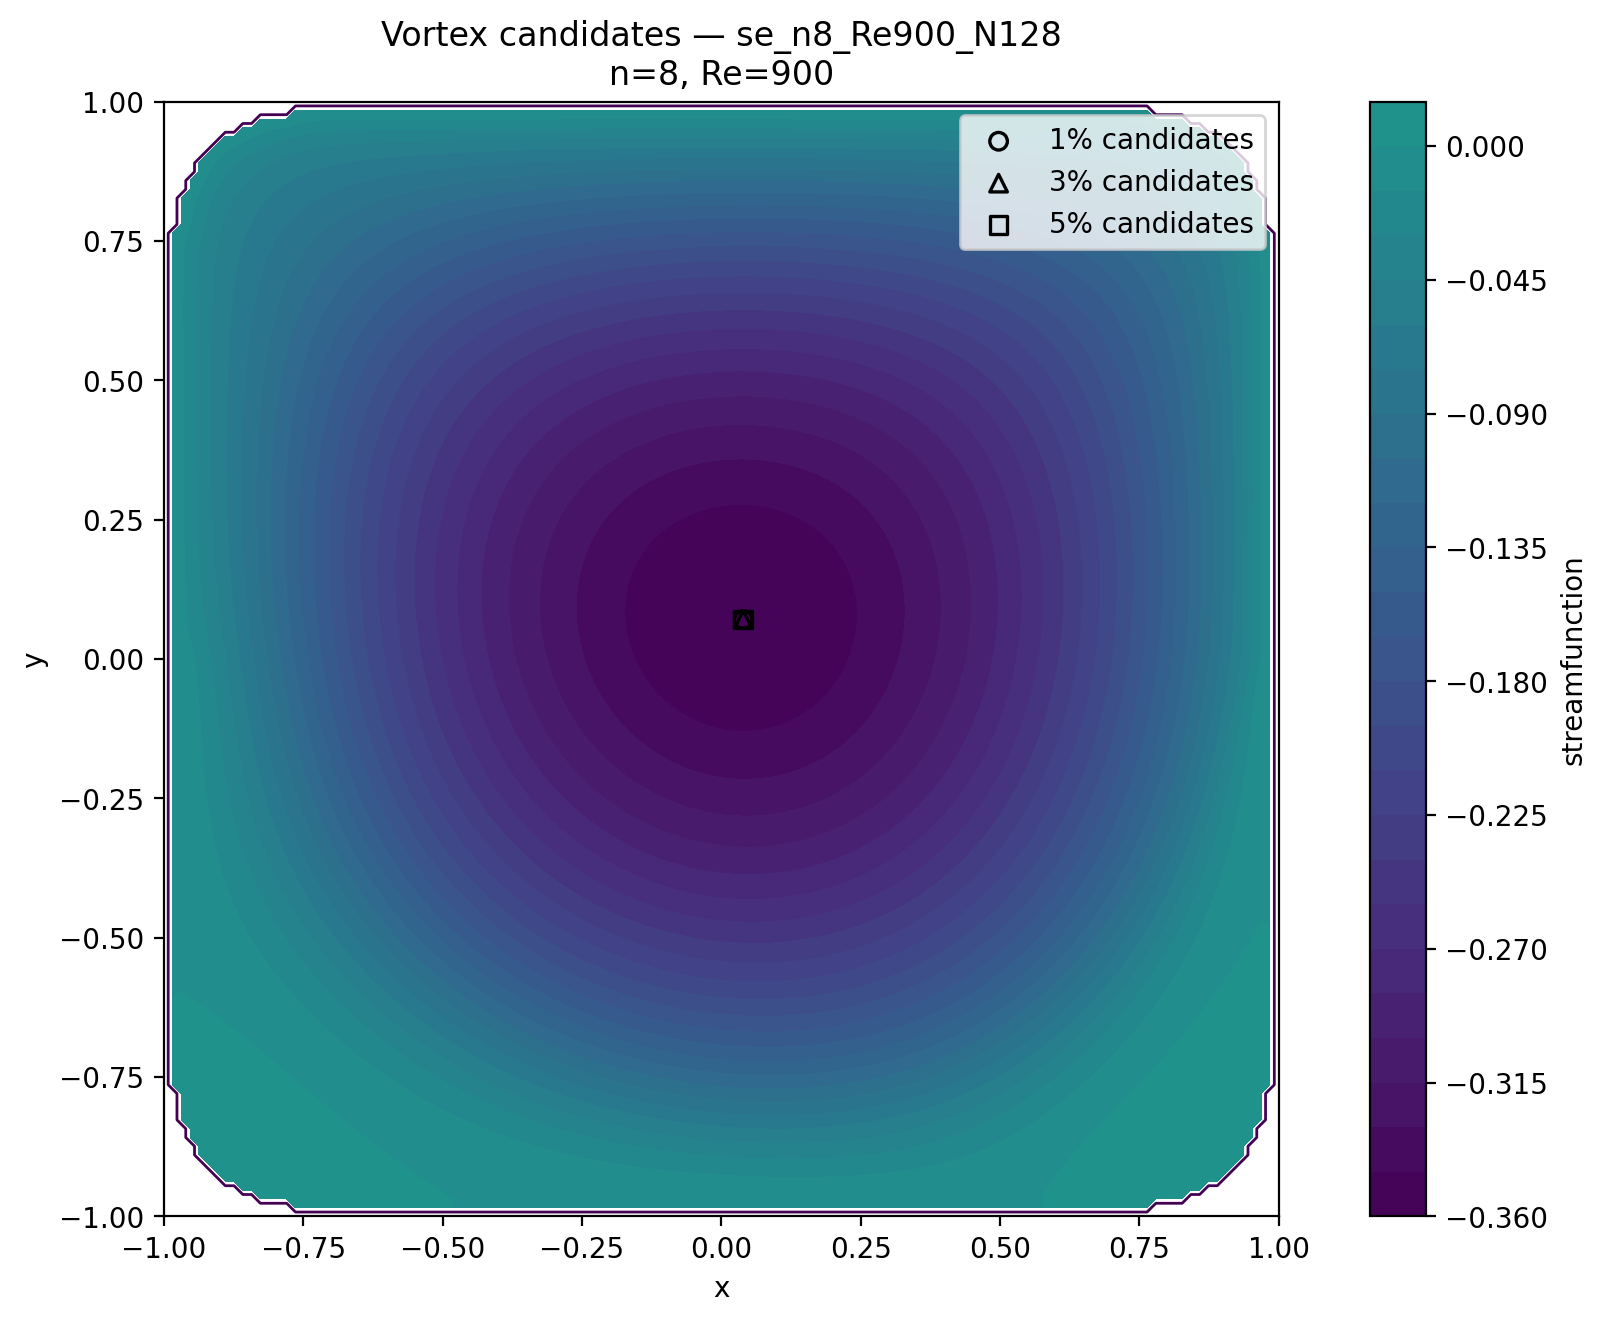
\includegraphics[width=\textwidth]{se_n8p0_Re900_N128_vortices.png} \caption{$n=8,\;Re=900$ --- one extremum} \end{subfigure} \hfill \begin{subfigure}[b]{0.31\textwidth} 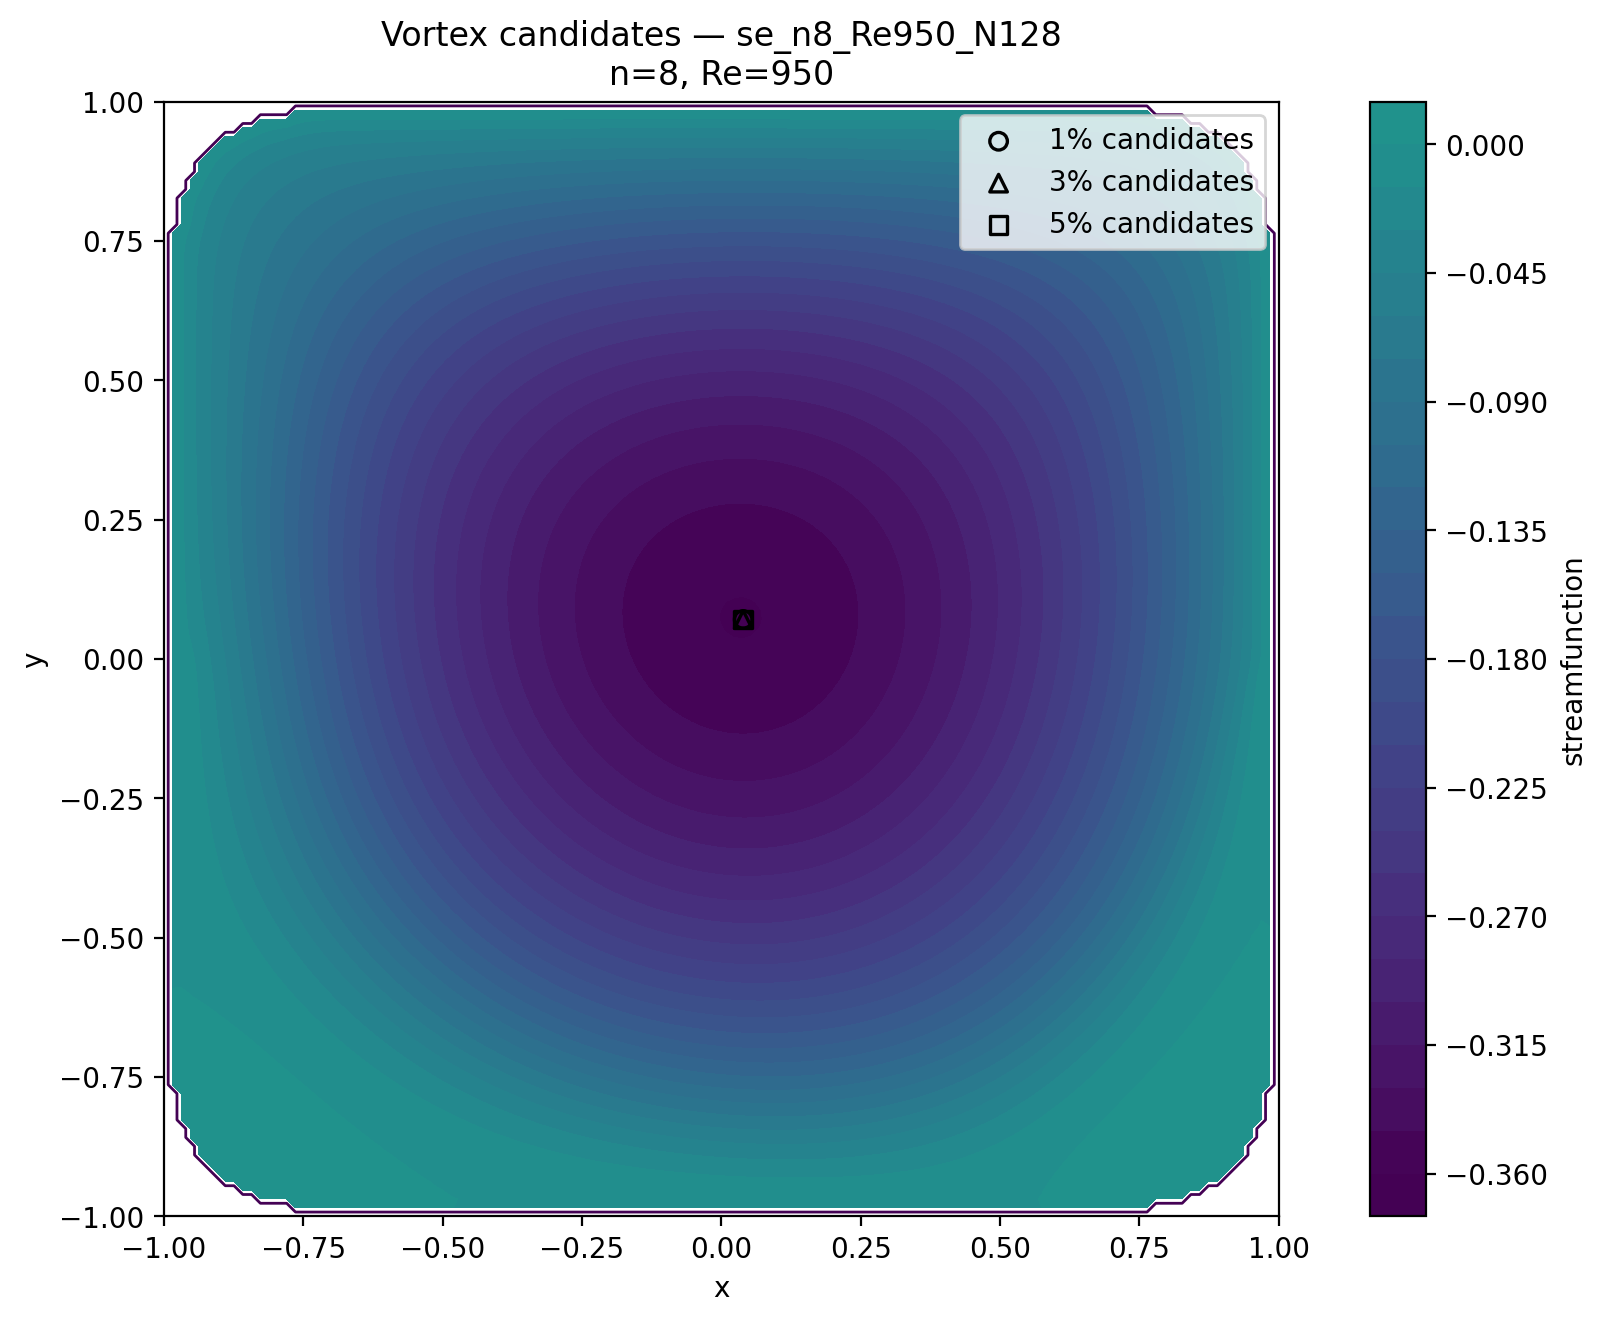
\includegraphics[width=\textwidth]{se_n8p0_Re950_N128_vortices.png} \caption{$n=8,\;Re=950$ --- one extremum} \end{subfigure} \hfill \begin{subfigure}[b]{0.31\textwidth} 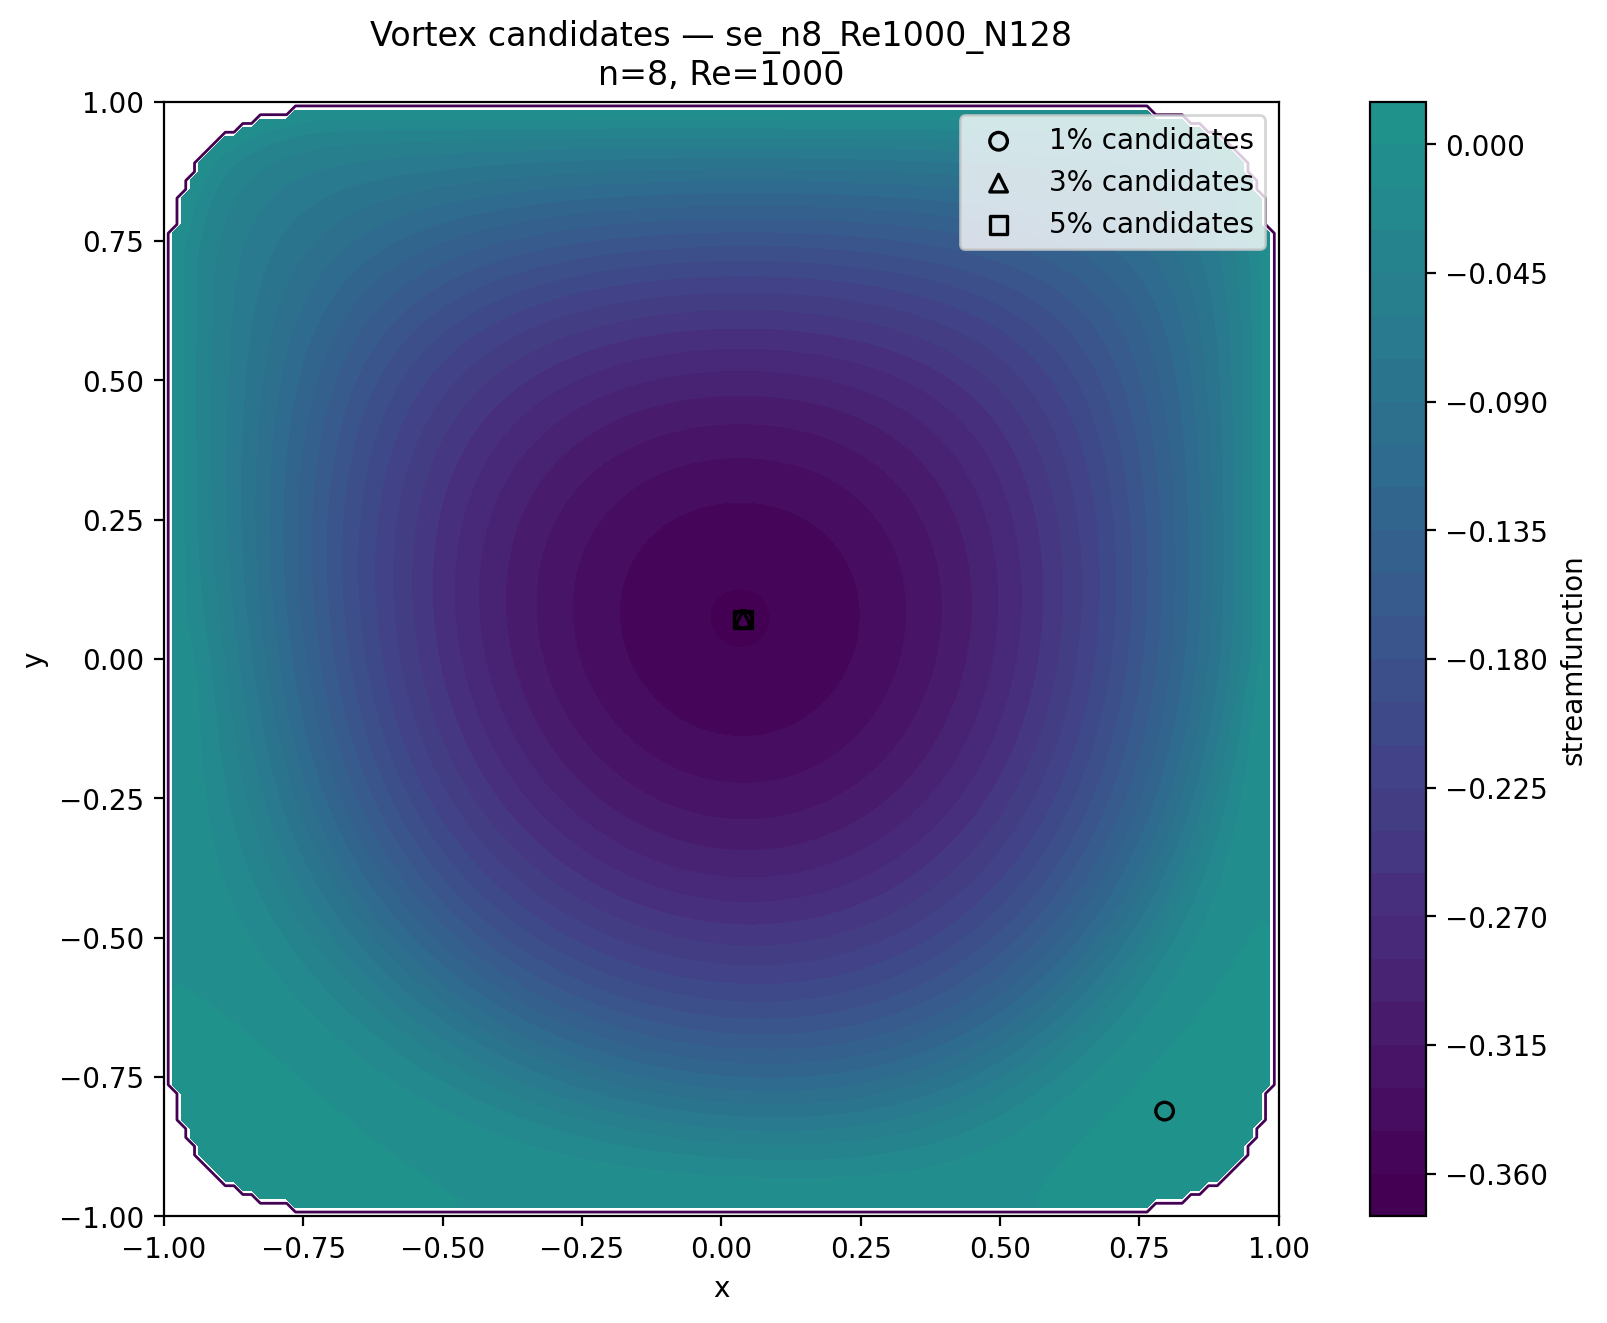
\includegraphics[width=\textwidth]{se_n8p0_Re1000_N128_vortices.png} \caption{$n=8,\;Re=1000$ --- two extrema} \end{subfigure}
\caption{Secondary corner extremum at $n=8$. Of the 190 cases on the grid, one
resolves a second extremum above the $1\%$ threshold of the primary circulation.
At $N=128$, the count changes from one to two between $Re=950$ and $Re=1000$;
this is a $1\%$ detection-threshold crossing bracket.}




\label{fig:cornerbracket}
\end{figure}


\section{Targeted projected-lid control}\label{sec:lidlaw}
The reference forcing is the tangential law
$\mathbf{u}_{\rm lid}=U_{\rm lid}(m_y,-m_x)$ on the upper arc. For comparison
with conventional square-cavity implementations one may define a projected
tangential law by taking a horizontal translation $\mathbf{e}_x$ and projecting
it onto the local tangent,
$\mathbf{u}_{\rm lid}^{\rm proj}=U_{\rm lid}(\mathbf{e}_x\cdot\mathbf{t})\mathbf{t}$,
with $\mathbf{t}=(m_y,-m_x)$. This law is impermeable and reduces exactly to the
classical uniform lid on a straight horizontal edge. It also removes the
reference-law velocity discontinuity: $\mathbf{u}_{\rm lid}^{\rm proj}\cdot e_x
=U_{\rm lid}m_y^2\to0$ at $(\pm1,0)$, so the projected velocity approaches the
stationary lower arc continuously. It is therefore a coupled forcing and
junction control, not an isolated geometry perturbation.

The targeted control covers $n=1.5,2,4,8$ at $Re=100$ and $Re=1000$ on $N=128$,
plus $n=4$ at $Re=100$ and all four exponents at $Re=1000$ on $N=256$: $13$
converged design fields in total. Ten projected fields were computed for this
revision and three earlier $N=128$, $Re=1000$ fields at $n=2,4,8$ were reused.
All stopping residuals lie in $7.73\times10^{-9}$--$1.00\times10^{-8}$. Each
projected field is paired with the tangential field at the same $(n,Re,N)$,
$U_{\rm lid}=0.05$, Mach number and superelliptic geometry; only the imposed
wall-velocity direction changes. The comparison uses the production
convention $D=2\int_M(2S:S/Re)\,dA$ and $D/A_{\rm mask}=D/\mathrm{card}(M)dx^2$,
while $KE/A$ uses the exact geometric area. Relative $L_2(u)$ is evaluated on
the common fluid support.

\begin{table}[H]
\centering
\caption{Targeted tangential/projected lid comparison. Ratios are projected
over tangential; $D/A_{\rm mask}$ uses the gradient-valid area and $KE/A$ uses
the exact geometric area. The last column divides the $D/A$ ratio by the
$\int u_{\rm lid}^2ds$ ratio ($0.5$ on the sampled geometries), giving a direct
forcing-normalized comparison. The velocity norm uses the common fluid
support.}
\label{tab:projtarget}
\tabbox{\begin{tabular}{@{}rrrcccccccr@{}}
\toprule
$N$ & $Re$ & $n$ & $D/A_{\rm mask}$ tan. & $D/A_{\rm mask}$ proj. & raw ratio &
forcing-norm.\ ratio & $KE/A$ ratio & $f_{0.25}$ ratio & $U_{\max}$ ratio & rel. $L_2(u)$ \\
\midrule
128 & 100 & 1.5 & 0.05360 & 0.02095 & 0.391 & 0.782 & 0.509 & 0.700 & 0.957 & 0.333 \\
128 & 100 & 2.0 & 0.03814 & 0.01820 & 0.477 & 0.955 & 0.485 & 0.770 & 0.982 & 0.394 \\
128 & 100 & 4.0 & 0.03412 & 0.02630 & 0.771 & 1.542 & 0.421 & 1.076 & 0.991 & 0.517 \\
128 & 100 & 8.0 & 0.04047 & 0.03577 & 0.884 & 1.768 & 0.386 & 1.353 & 0.983 & 0.577 \\
128 & 1000 & 1.5 & 0.01073 & 0.00474 & 0.442 & 0.883 & 0.512 & 0.847 & 0.941 & 0.306 \\
128 & 1000 & 2.0 & 0.00835 & 0.00451 & 0.539 & 1.079 & 0.494 & 0.923 & 0.974 & 0.334 \\
128 & 1000 & 4.0 & 0.00714 & 0.00562 & 0.786 & 1.572 & 0.457 & 1.327 & 0.952 & 0.404 \\
128 & 1000 & 8.0 & 0.00755 & 0.00644 & 0.853 & 1.707 & 0.436 & 1.449 & 0.953 & 0.446 \\
256 & 100 & 4.0 & 0.03940 & 0.02820 & 0.716 & 1.431 & 0.422 & 0.920 & 0.997 & 0.518 \\
256 & 1000 & 1.5 & 0.01353 & 0.00551 & 0.408 & 0.815 & 0.511 & 0.841 & 0.974 & 0.306 \\
256 & 1000 & 2.0 & 0.01029 & 0.00529 & 0.514 & 1.028 & 0.495 & 0.894 & 0.990 & 0.334 \\
256 & 1000 & 4.0 & 0.00880 & 0.00702 & 0.798 & 1.596 & 0.460 & 1.195 & 0.984 & 0.406 \\
256 & 1000 & 8.0 & 0.00920 & 0.00834 & 0.906 & 1.813 & 0.437 & 1.307 & 0.988 & 0.450 \\
\bottomrule
\end{tabular}
}
\end{table}


\begin{figure}[H]
\centering
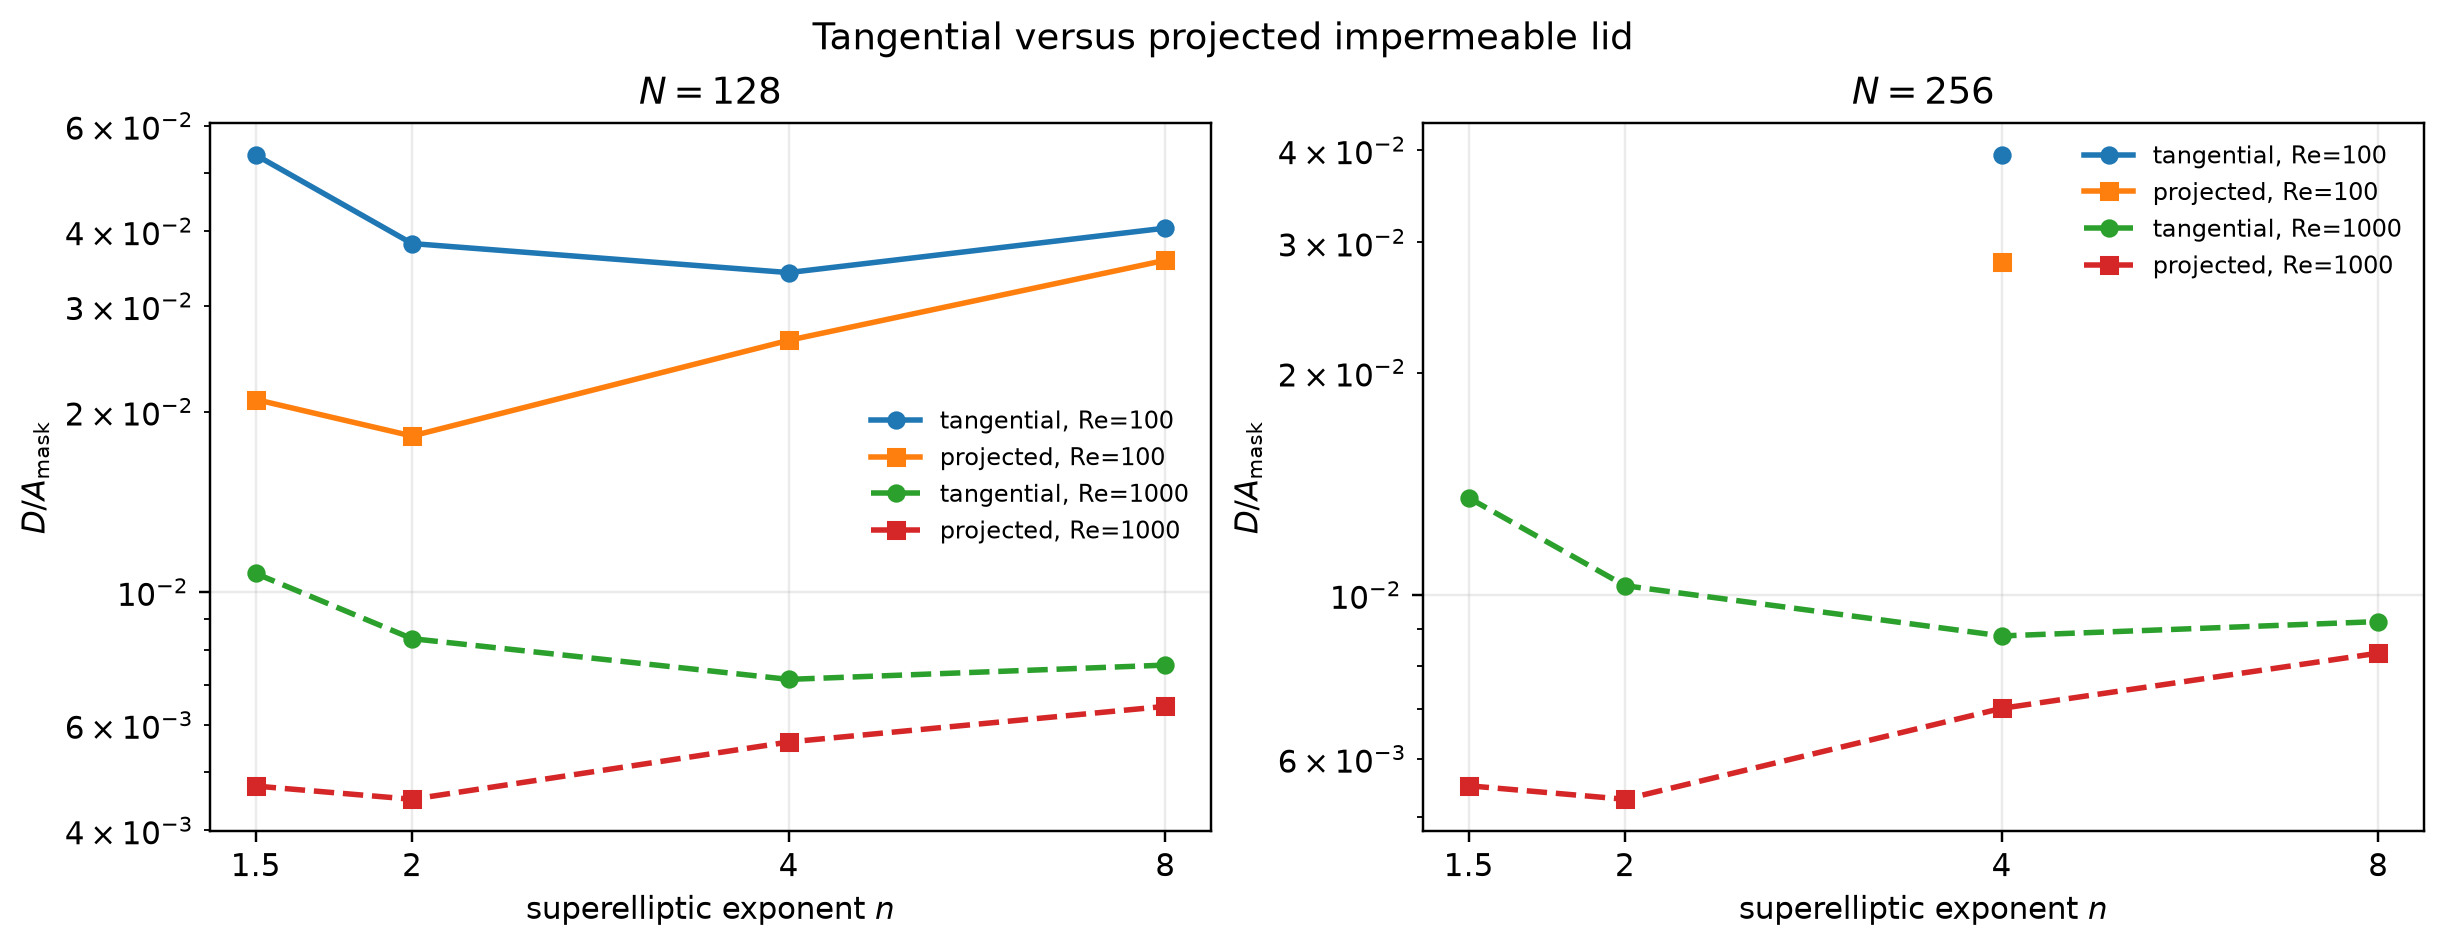
\includegraphics[width=0.98\textwidth]{fig_lid_projected_targeted.png}
\caption{Dissipation density versus $n$ for the tangential and projected lid
laws: (a) $N=128$ and (b) $N=256$; (c) forcing-normalized $D/A$ ratio (raw
ratio divided by $0.5$), with the dotted line at unity. Solid lines are
$Re=100$, dashed lines are $Re=1000$; circles denote tangential and squares
projected results in (a,b), while markers in (c) distinguish $N=128$ (circles)
from $N=256$ (squares). The sampled low-loss band moves toward $n=2$, but the
projected continuous argmin is only bracketed by the sampled exponents $n=1.5$
and $n=4$.}
\label{fig:projtarget}
\end{figure}


The projected law lowers raw $D/A_{\rm mask}$ at every sampled design, with
projected/tangential ratios of $0.391$--$0.906$ (Table~\ref{tab:projtarget}).
The raw ratio, however, compares unequal forcings. For the sampled
superellipses,
\[
  \frac{\int_{\Gamma_{\rm mov}}|\mathbf{u}_{\rm lid}^{\rm proj}|^2ds}
       {\int_{\Gamma_{\rm mov}}|\mathbf{u}_{\rm lid}|^2ds}
  =\frac{\int_{\Gamma_{\rm mov}}m_y^2ds}{\int_{\Gamma_{\rm mov}}ds}
  =\frac12 ,
\]
so direct normalization by the imposed boundary-velocity integral changes the
ratio to $0.782$--$1.813$. Normalization by the measured $KE/A$ ratio instead
gives $0.768$--$2.291$, because $KE/A$ includes the bulk response and is not a
prescribed forcing norm. Both normalizations are reported because they answer
different questions; neither turns this paired run into an isolation of
geometry. The sampled minimum moves from $n=4$ to $n=2$ on the three complete
ladders, but the sampled set is only $\{1.5,2,4,8\}$. The continuous projected
argmin is therefore bracketed between $n=1.5$ and $n=4$; no optimum at exactly
$n=2$ is resolved. The raw depth falls from $36.4\%$ to $13.1\%$ at $N=128$,
$Re=100$, from $33.4\%$ to $5.0\%$ at $N=128$, $Re=1000$, and from $35.0\%$ to
$4.1\%$ at $N=256$, $Re=1000$. Near-wall dissipation is not uniformly reduced:
the $f_{0.025}=D_\delta/D$ ratio spans $0.700$--$1.449$ with
$\delta=0.025L_c$, and the relative field difference spans $0.306$--$0.577$.
Here ``depth'' is
$100\,[1-D/A(n_{\rm argmin})/D/A(n=1.5)]$, so it measures the sampled drop
from the smallest tested exponent rather than a drop from an asymptotic
reference.

Resolution drift is not removed by eliminating the tangential-law junction
jump. At $Re=1000$, the $N=256/N=128$ change in $D/A_{\rm mask}$ under the
projected law is $+16.3\%$, $+17.3\%$, $+25.0\%$ and $+29.5\%$ at
$n=1.5,2,4,8$; the paired tangential values are $+26.1\%$, $+23.2\%$,
$+23.1\%$ and $+21.9\%$. The projected family therefore drifts as much as, and
at the two largest exponents more than, the discontinuous family. The junction
velocity jump alone cannot explain the resolution sensitivity; near-wall
gradients and bulk discretization remain plausible contributors. The largest
fixed-junction-disk comparison still leaves $4.33$--$14.28\%$ drift. The
diffusive-scaling test described in Sec.~\ref{sec:diffusive} shows that lowering
the lattice Mach number changes part of this drift but does not eliminate it, so
no Mach/acoustic explanation is established. The sampled shifts and
ratios remain descriptive diagnostics within this coupled family; no universal
optimum or verified lid-power balance follows from them.

\section{Detailed tables moved from the main article}
\label{sec:moved}
The following four tables collect the detailed observable, fit-window,
crossing and finite-element diagnostics that support compact statements in the
main article. They are retained here so that the main text can present the
physical argument without interrupting it with long numerical tables. The
common-support LBM/FEM values of the former main-text table are already given
in Table~\ref{tab:commonsupport} and are not duplicated.

\begin{table}[H]
\centering
\caption{Integrated kinetic energy at $Re=1000$, $N=128$, with the two area
normalizations kept distinct.}
\label{tab:kinetic_moved}
\tabbox{\begin{tabular}{@{}ccccc@{}}
\toprule
$n$ & $KE$ & $KE/A_{\rm fluid}$ & $KE/A(n)$ & $U_{\max}/U_{\rm lid}$ \\
\midrule
1.25 & 0.24607 & 0.10149 & 0.10138 & 1.000 \\
1.5 & 0.30414 & 0.11125 & 0.11109 & 1.000 \\
1.75 & 0.34539 & 0.11649 & 0.11638 & 0.999 \\
2 & 0.37134 & 0.11842 & 0.11820 & 0.997 \\
2.5 & 0.39864 & 0.11812 & 0.11791 & 1.027 \\
3 & 0.40901 & 0.11621 & 0.11576 & 1.039 \\
4 & 0.41859 & 0.11352 & 0.11288 & 1.039 \\
5 & 0.42159 & 0.11169 & 0.11093 & 1.035 \\
6 & 0.42110 & 0.11011 & 0.10923 & 1.031 \\
8 & 0.42083 & 0.10855 & 0.10752 & 1.027 \\
\bottomrule
\end{tabular}}
\end{table}


\begin{table}[H]
\centering
\caption{Fit-window sensitivity on matched fields. Supports, exclusions and
the estimator are described in Sec.~\ref{sec:fits}; a dash means the vertex was
rejected.}
\label{tab:fit_moved}
\tabbox{\begin{tabular}{@{}lcccrrr@{}}
\toprule
grid & $Re$ & quantity & sampled argmin & 3-point $n^*$ & 5-point $n^*$ \\
\midrule
$N=128$ & 300  & $D/A_{\rm mask}$ & 3.5  & 3.411 & 3.442 \\
$N=128$ & 300  & $D$              & 2.5  & 2.600 & 2.599 \\
$N=128$ & 500  & $D/A_{\rm mask}$ & 3.5  & 3.538 & 3.624 \\
$N=128$ & 500  & $D$              & 2.75 & 2.680 & 2.598 \\
$N=128$ & 1000 & $D/A_{\rm mask}$ & 4    & 4.065 & 4.471 \\
$N=128$ & 1000 & $D$              & 3    & 2.794 & 2.381 \\
\midrule
$N=256$ & 300  & $D/A_{\rm mask}$ & 3.5  & 3.471 & 3.521 \\
$N=256$ & 300  & $D$              & 2.5  & 2.536 & 2.598 \\
$N=256$ & 500  & $D/A_{\rm mask}$ & 3.75 & 3.692 & 3.685 \\
$N=256$ & 500  & $D$              & 2.5  & 2.561 & 2.623 \\
$N=256$ & 1000 & $D/A_{\rm mask}$ & 3.75 & 3.825 & 3.995 \\
$N=256$ & 1000 & $D$              & 2.5  & 2.613 & 2.670 \\
\bottomrule
\end{tabular}}
\end{table}


\begin{table}[H]
\centering
\caption{Bracketed crossings of adjacent-exponent ratios. ``No crossing''
means the ratio keeps its sign over the available bracket; the estimator is
linear interpolation of $\log$(ratio).}
\label{tab:crossing_moved}
\tabbox{\begin{tabular}{@{}llllcc@{}}
\toprule
grid & quantity & exponents & $Re_{\rm cross}$ & bracket & endpoint ratios \\
\midrule
$N=128$ all190 & $D/A_{\rm mask}$ & $3/4$ & $338.2$ & $300$--$350$ & $0.9980$, $1.0006$ \\
$N=128$ union & $D/A_{\rm mask}$ & $3/4$ & $337.6$ & $325$--$350$ & $0.9994$, $1.0006$ \\
$N=256$ union & $D/A_{\rm mask}$ & $3/4$ & $272.2$ & $250$--$300$ & $0.9989$, $1.0014$ \\
$N=384$ extB & $D/A_{\rm mask}$ & $3/4$ & $228.3$ & $200$--$250$ & $0.9983$, $1.0013$ \\
$N=512$ extB & $D/A_{\rm mask}$ & $3/4$ & $199.2$ & $150$--$200$ & $0.9963$, $1.0001$ \\
\midrule
$N=128$ union & $D$ & $2.5/3$ & $892.9$ & $875$--$900$ & $0.9998$, $1.0001$ \\
$N=256$ union & $D$ & $2.5/3$ & no crossing & -- & $0.9848$, $0.9966$ \\
$N=384$ extB & $D$ & $2.5/3$ & no crossing & -- & $0.9849$, $0.9885$ \\
$N=512$ extB & $D$ & $2.5/3$ & no crossing & -- & $0.9852$, $0.9885$ \\
\bottomrule
\end{tabular}}
\end{table}


\begin{table}[H]
\centering
\caption{Directly integrated FEM dissipation at $Re=1000$ for mesh levels
$n_{\rm ref}=4,5,6$, with the lattice reconstruction diagnostics at $N=128$.
The mesh change is reported directly; no Richardson estimate is used.}
\label{tab:fem_moved}
\tabbox{\begin{tabular}{@{}cccccc@{}}
\toprule
$n$ & $D_{4}$ & $D_{5}$ & $D_{6}$ & $\epsilon_{\nabla u}$ & rel. $D$ error \\
\midrule
1.25 & 0.055193 & 0.059007 & 0.062231 & 6.3\% & 1.4\% \\
2 & 0.047212 & 0.047671 & 0.049404 & 4.9\% & 1.0\% \\
4 & 0.050261 & 0.049286 & 0.050635 & 5.0\% & 1.1\% \\
8 & 0.056177 & 0.054124 & 0.054848 & 5.6\% & 1.4\% \\
\bottomrule
\end{tabular}}
\end{table}


\begin{table}[H]
\centering
\caption{Fixed-junction-disk dissipation $D_{r_0}(N)$ for $n=8$, $Re=1000$,
computed from the archived final fields, including the $N=384$ high-resolution
field. Here $r_0=0$ denotes the unexcised gradient-valid mask.}
\label{tab:dr0ladder}
\tabbox{\begin{tabular}{@{}lccccc@{}}
\toprule
$N$ & $h$ & $D_{r_0=0}$ & $D_{r_0=0.125}$ & $D_{r_0=0.25}$ & $D_{r_0=0.5}$ \\
\midrule
64  & 0.031746 & 0.020732 & 0.019702 & 0.017604 & 0.013966 \\
128 & 0.015748 & 0.028391 & 0.025734 & 0.022968 & 0.018243 \\
256 & 0.007843 & 0.035312 & 0.030362 & 0.026487 & 0.020849 \\
384 & 0.005222 & 0.038940 & 0.032227 & 0.027872 & 0.021891 \\
512 & 0.003914 & 0.041172 & 0.033132 & 0.028510 & 0.022360 \\
\bottomrule
\end{tabular}}
\end{table}


\begin{table}[H]
\centering
\caption{Equal-doubling increments (in $10^{-6}$), observed orders and
Richardson limits for the $n=8$, $Re=1000$ fixed-junction-disk ladder. Orders
use the $64/128/256/512$ subset; the $N=384$ row of Table~\ref{tab:dr0ladder}
is an intermediate point and is not used in the equal-doubling ratios.}
\label{tab:dr0order}
\tabbox{\begin{tabular}{@{}lcccccc@{}}
\toprule
$r_0$ & $\Delta_{64\to128}$ & $\Delta_{128\to256}$ & $\Delta_{256\to512}$ &
$p_{128/256}$ & $p_{256/512}$ & $D_\infty^{\rm Rich}$ \\
\midrule
$0$     & $7658$ & $6922$ & $5859$ & $0.15$ & $0.24$ & --- \\
$0.125$ & $6032$ & $4628$ & $2770$ & $0.38$ & $0.74$ & $0.0373$ \\
$0.25$  & $5364$ & $3518$ & $2024$ & $0.61$ & $0.80$ & $0.0313$ \\
$0.5$   & $4277$ & $2606$ & $1511$ & $0.71$ & $0.79$ & $0.0244$ \\
\bottomrule
\end{tabular}}
\end{table}


\begin{figure}[H]
\centering
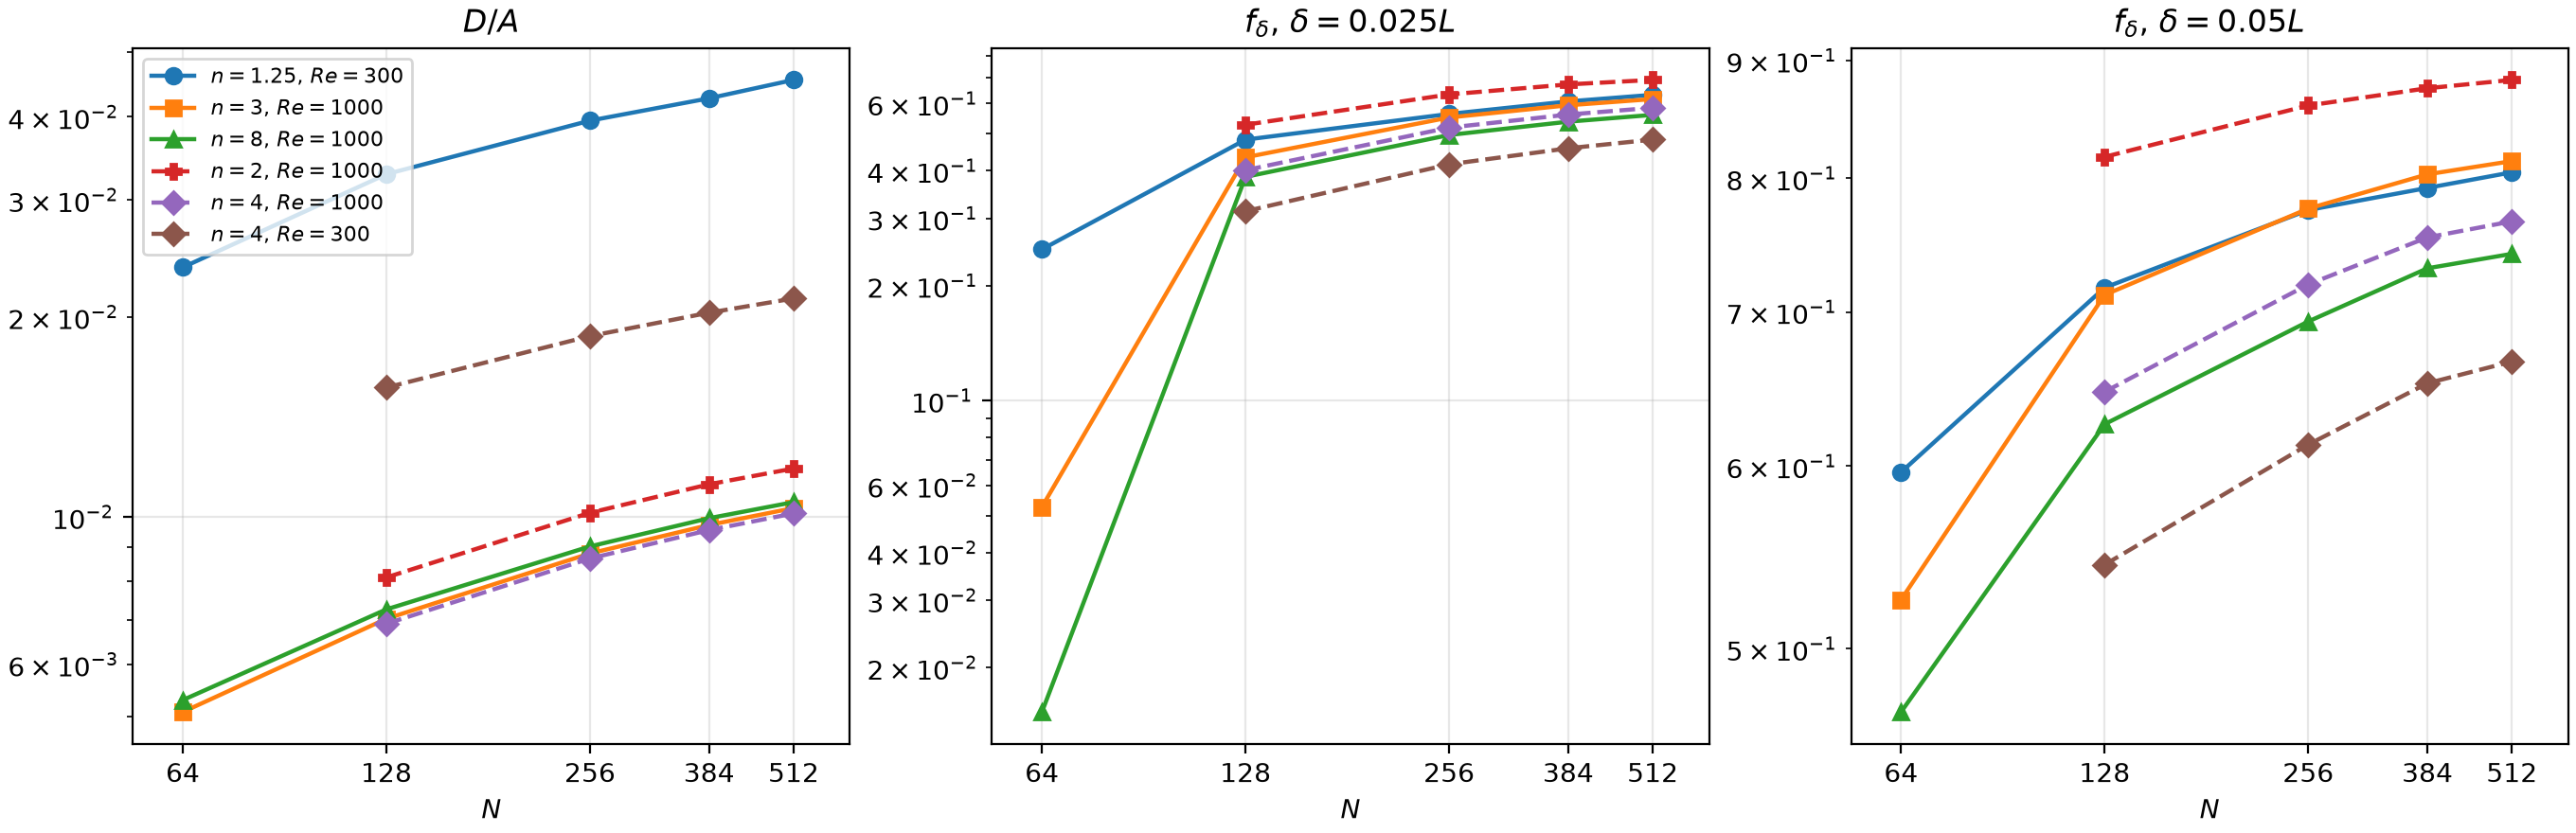
\includegraphics[width=0.98\textwidth]{convergence_paroi.png}
\caption{Resolution sensitivity of the near-wall diagnostics on the archived
$N=64,128,256$ ladder. The three sampled cases are $(n,Re)=(1.25,300)$,
$(3,1000)$ and $(8,1000)$; the panels show $D/A_{\rm mask}$ and the wall-band
shares for $\delta=0.025L_c$ and $\delta=0.05L_c$. These curves support ordering
of the sampled diagnostics only; no asymptotic rate or grid-converged amplitude
is claimed.}
\label{fig:wallrefine}
\end{figure}


\section{Production-family diffusive-scaling check}
\label{sec:diffusive}
To test whether the residual resolution drift of the production family is a
lattice-Mach effect, we reran the $n=4$, $Re=1000$ cases at $N=128,256,384,512$
with $U_{\mathrm{lid}}(N)=0.05\times128/N$ and nearly fixed
$\tau\simeq0.519$. The lattice Mach number therefore decreases as $1/N$, while
$Re$ and the gradient-valid quadrature are unchanged. Table~\ref{tab:diffusive}
compares these fields with the original production fields at the same physical
junction radii. The $N=128$ fields agree by construction because $U_{\rm lid}$
and $\tau$ match. At $r_0=0.5$ the diffusive values agree with the production
values to within $5.3\times10^{-6}$ on $N=128$--$512$, and the increments on
$128\to256$, $256\to384$ and $384\to512$ remain $2.06\times10^{-3}$,
$6.85\times10^{-4}$ and $3.21\times10^{-4}$ (observed order about $1.01$ on $128/256/384$; the diffusive ladder
gives $1.01$ and an increment-ratio order of $2.69$). Lowering
the lattice Mach number changes the unexcised full-domain level appreciably but
leaves the junction-excised values essentially unchanged; it does not remove the
resolution drift. This check is not a continuum certification. It only excludes
a simple Mach/acoustic explanation of the remaining drift.

\begin{table}[H]
\centering
\caption{Production-family diffusive-scaling check at $n=4$, $Re=1000$:
$U_{\mathrm{lid}}(N)=0.05\times128/N$ and nearly fixed $\tau\simeq0.519$.
$D_{\rm prod}$ and $D_{\rm diff}$ denote the original production fields and the
diffusively scaled reruns; $r_0$ is the physical junction-disk radius, with
$r_0=0$ the unexcised gradient-valid mask.}
\label{tab:diffusive}
\tabbox{\begin{tabular}{@{}lccccccccc@{}}
\toprule
$N$ & $U_{\rm lid}$ & $\tau$ & $D_{\rm prod}(0)$ & $D_{\rm diff}(0)$ &
$D_{\rm prod}(0.25)$ & $D_{\rm diff}(0.25)$ &
$D_{\rm prod}(0.5)$ & $D_{\rm diff}(0.5)$ \\
\midrule
128 & 0.05000 & 0.519050 & 0.025590 & 0.025590 & 0.020028 & 0.020029 & 0.015117 & 0.015117 \\
256 & 0.02500 & 0.519125 & 0.032090 & 0.032623 & 0.023007 & 0.023001 & 0.017179 & 0.017176 \\
384 & 0.01667 & 0.519150 & 0.035407 & 0.036158 & 0.024015 & 0.024008 & 0.017864 & 0.017859 \\
512 & 0.01250 & 0.519162 & 0.037509 & 0.038374 & 0.024482 & 0.024473 & 0.018184 & 0.018179 \\
\bottomrule
\end{tabular}}
\end{table}



\subsection*{Fixed-physical-wall-support diagnostic}
To separate a wall-support effect from a resolved-gradient drift, we recomputed
$D$ on $M\cap\{\mathrm{dist}(x,\Gamma)>\delta\}$ for $n=4$, $Re=1000$,
$N=128$--$512$, with $\delta=0.05L_c$ and $0.10L_c$. The distance to $\Gamma$
($n=4$, $a=b=1$, $L_c=2$) is evaluated by a dense boundary sampling and a
KD-tree query in physical coordinates, so it does not depend on the lattice
spacing. Table~\ref{tab:dcore} reports $D_{\rm core}$ and the complementary
wall contribution; additivity $D_{\rm core}+D_{\rm wall}=D_M$ is exact. The
junction-excised $D_{r_0=0.5}$ increases by $16.9\%$ from $N=128$ to $512$ and
retains an observed order of about $1.01$ (equal-doubling order $1.04$),
whereas $D_{\rm core}$ changes by only $2.8\%$ at $\delta=0.05L_c$ and $6.7\%$
at $\delta=0.10L_c$ and shows no positive fitted order. The remaining
resolution drift is therefore associated with the near-wall support that
remains after junction excision, not with a first-order drift of the core
gradients on a fixed physical support. This diagnostic is not a continuum
certification.

\begin{table}[H]
\centering
\caption{Dissipation on a core support of fixed physical wall thickness, $D_{\rm core}(\delta)=2\nu\sum_{M\cap\{\mathrm{dist}(x,\Gamma)>\delta\}}S:S\,\Delta x^2$, with $\mathrm{dist}$ the exact distance to the superellipse boundary ($n=4$, $Re=1000$). $\delta=0.05$ and $0.1$ ($L_c=2$). Observed orders use successive doublings. This diagnostic separates the wall-support effect from the resolved-gradient drift and is not a continuum certification.}
\label{tab:dcore}
\tabbox{% Generated by scripts/final_revision/dcore_test.py
\begin{tabular}{@{}lcccccc@{}}
\toprule
$N$ & $D_M$ & $D_{\rm core}(0.05L_c)$ & $D_{\rm core}(0.10L_c)$ & $D_{\rm wall}(0.05L_c)$ & $D_{\rm wall}(0.10L_c)$ \\
\midrule
128 & 0.025590 & 0.008958 & 0.002817 & 0.016632 & 0.022772 \\
256 & 0.032090 & 0.008796 & 0.002675 & 0.023294 & 0.029415 \\
384 & 0.035407 & 0.008674 & 0.002645 & 0.026733 & 0.032763 \\
512 & 0.037509 & 0.008714 & 0.002641 & 0.028794 & 0.034868 \\
\bottomrule
\end{tabular}
}
\end{table}

\section*{Data availability}
The post-processed data, analysis scripts, regenerated figures, result tables,
the final supplementary document and a description of the directory structure
are publicly available at
\url{https://github.com/Ahmedalgeria778/PH13_revision_data}. The repository
does not contain the manuscript source or the raw simulation fields. It is
distributed under the MIT License; see the \texttt{LICENSE} and \texttt{README.md}
files in the repository.

\end{document}


